	\documentclass[11pt]{article}
\usepackage{mathrsfs}
%\documentclass[11pt,draftcls,onecolumn]{IEEEtran}
%\documentclass[9pt,twocolumn,twoside]{IEEEtran}
\usepackage{amsmath, alltt}
\usepackage{comment} % Load the package
\usepackage{rotating}
\usepackage{graphicx}
\usepackage{hyperref}
\usepackage{subfigure}
\usepackage[onehalfspacing]{setspace}
%\usepackage[doublespacing]{setspace}
\usepackage[hmargin={1.0in, 1.0in}, vmargin={1.0in, 1.0in}]{geometry}
\usepackage{amsfonts}
\usepackage{amssymb}
\usepackage{booktabs}
\usepackage{hhline}
\usepackage{natbib}
\usepackage{amsmath}
\usepackage{bm}
\usepackage{latexsym}
\usepackage{amssymb,bm}
\usepackage[section]{placeins}
\usepackage{longtable}
\usepackage{lscape}
\usepackage{scalefnt}
\usepackage{setspace}
\usepackage{xcolor}
\usepackage{mathtools}
\usepackage{authblk}

\usepackage{enumitem}
\usepackage[utf8]{inputenc}
\usepackage{geometry,booktabs,multirow,array,graphicx}
\usepackage{float}
\usepackage{algorithm}
\usepackage{algpseudocode}
\usepackage{lineno}

\newcommand{\purple}[1]{\textcolor{purple}{#1}}

% ---------------------------------------------------------------------------
% Revision markup (remove before final submission):
%   \rev{...}      : text revised/added in response to the referee reports (blue)
%   \authnote{...} : items the authors need to confirm (red, in brackets)
%   \todonote{...} : items the authors need to conduct (purple, in brackets)
% ---------------------------------------------------------------------------
\newcommand{\rev}[1]{{\color{blue}#1}}
\newcommand{\todonote}[1]{{\color{purple}[\textbf{Things to do:} #1]}}
\newcommand{\authnote}[1]{{\color{red}[\textbf{Note to authors:} #1]}}

%\pdfminorversion=4
% NOTE: To produce blinded version, replace "0" with "1" below.
\newcommand{\blind}{1}

% DON'T change margins - should be 1 inch all around.
%\addtolength{\oddsidemargin}{-.5in}%
%\addtolength{\evensidemargin}{-.5in}%
%\addtolength{\textwidth}{1in}%
%\addtolength{\textheight}{-.3in}%
%\addtolength{\topmargin}{-.8in}%

\newcommand{\pg}{\it\color{red}}
\newcommand{\gp}{\rm\color{black}}
\newcommand{\harpoon}{\overset{\rightharpoonup}}

\DeclareMathOperator*{\argmax}{arg\,max}

%\usepackage{tikz}
%\usetikzlibrary{shapes,arrows}
%\usepackage[latin1]{inputenc}


\begin{document}
\linenumbers
	\setlength{\abovedisplayskip}{6pt}
	\setlength{\belowdisplayskip}{6pt}
	\setlength{\abovedisplayshortskip}{6pt}
	\setlength{\belowdisplayshortskip}{6pt}	
%\def\spacingset#1{\renewcommand{\baselinestretch}%
%	{#1}\small\normalsize} \spacingset{1}
\if1\blind
{
	\title{Insurance Ratemaking with Endogenous Deductibles}	
\author[1]{Dongha Lee}
\author[2]{Hangsuck Lee}
\author[1,3,*]{Himchan Jeong}
\affil[1]{\small Department of Statistics and Actuarial Science, Simon Fraser University}
\affil[2]{\small Department of Mathematics/Actuarial Science, Sungkyunkwan University}
\affil[3]{\small Department of Next Generation Smart Energy System Convergence, Gachon University}
\affil[*]{Corresponding author: Himchan Jeong / Email: \url{himchan_jeong@sfu.ca}}


	\date{}	
	\maketitle
} \fi


\begin{abstract}
\rev{This article examines insurance ratemaking with an endogenous deductible. While the deductible has been assumed to be exogenous to the claim frequency and severity in classical nonlife insurance ratemaking practice, its endogeneity has been argued in terms of policyholders' behaviour and information asymmetry between policyholders and insurers. Moreover, the presence of a deductible also determines what the insurer can observe: ground-up losses below the deductible are either recorded with a zero payment (censoring) or not recorded at all (truncation), so that the ground-up loss information available for ratemaking is incomplete.

In this context, we consider a joint modeling framework that captures possible dependence between the insurance claims and the endogenous deductible via pair copulas, in the presence of deductible-induced censoring and truncation of the ground-up loss information. The framework adapts the frequency and severity likelihoods to the censored and truncated observation mechanisms, and accommodates both continuous and discrete (ordinal) deductibles. A simulation study shows that the proposed joint models recover the true parameters with negligible bias under incomplete data, whereas the marginal models that ignore the endogeneity of the deductible can be substantially biased. Lastly, an empirical analysis using the LGPIF data shows that the endogeneity of the deductible is not ignorable and that the proposed framework yields a better risk classification model in terms of goodness-of-fit and out-of-sample prediction.}



\textbf{Keywords}: Dependence modeling, Endogenous deductible, Pair copula, Incomplete data, \rev{Censoring and truncation}

\end{abstract}
%
%\noindent
%{\it Keywords:} Compound distributions, Copula regression, Endogenous deductible, Incomplete data, Nonlife insurance
%

\newpage
%\spacingset{1.45} % DON'T change the spacing!
\section{Introduction}
\label{sec:intro}

Traditional actuarial practice historically determines the price, or net premium, of a nonlife insurance contract by assuming the contract deductible is exogenous, meaning the riskiness of policyholders is independent of the deductible level \citep{Klugman2012}. However, this assumption is fundamentally contradicted by contract theory, which posits that the deductible is determined endogenously in the optimal contract design to mitigate market inefficiency caused by information asymmetry between the policyholder and the insurer \citep{Bolton2005contract}. When policyholders possess private information about their expected loss costs, their choice of deductible is based on these hidden risks, making the deductible an endogenous factor in regressions modeling both claim frequency and claim severity. % Information asymmetry can take several forms that influence this dependence, notably adverse selection, where high-risk policyholders select lower deductibles and low risks select higher deductibles \citep{rothschild1976equilibrium, Holmstrom1979moral}. Furthermore, ex ante moral hazard contributes, as low-deductible policyholders are incentivized to underinvest in precaution \citep{Winter2013optimal}. Ex post moral hazard, such as policyholders underreporting or aggregating multiple losses into a single claim to surpass a high deductible, also creates a positive relationship between deductible and loss cost.

%To address the complexities arising from the endogeneity of the deductible and the structure of insurance losses, which are typically defined by a compound or stopped-sum distribution (the sum of individual claim amounts stopped by the number of claims), researchers have introduced sophisticated joint modeling frameworks.
 
Since the dependence between the deductible and the policyholder's risk requires separate treatment for claim frequency and claim severity, \citet{shi2022copula} consider pair copula constructions (or vine copulas) to jointly model the deductible, the number of claims (frequency), and individual claim amounts (severity). Note that copulas are widely used in the actuarial literature for modeling various dependence structures observed from the claim data \citep{FreesValdez1998, ShiLu2018, jeong2023multivariate}.

\rev{While the work of \citet{shi2022copula} adopts flexible dependence structures and allows insurers to better uncover the underlying risk distribution of potential customers, it assumes that the insurer observes the exact ground-up loss amount of every loss event, including the losses below the deductible. In practice, the presence of a deductible also determines what the insurer can observe. When a ground-up loss does not exceed the deductible, the insurer pays nothing, and the loss is either recorded as a claim with zero payment, so that the insurer only knows that a loss below the deductible occurred (censored data), or not recorded at all, so that the insurer is unaware of the occurrence of the loss (truncated data). The latter is the typical situation in practice, because policyholders have little motivation to report a loss when the amount to be recovered is small \citep{YipKarenC.H.2005Omcf}, and because a reported claim may affect the renewal premium under experience rating.

We emphasize that the incomplete data mechanisms considered in this article are deductible-induced censoring and truncation of the ground-up loss information: whether a loss is (fully) observed is determined by whether the ground-up loss exceeds the deductible. This is distinct from the behavioural forms of underreporting discussed in \citet{shi2022copula} as a possible source of the endogeneity of the deductible, such as ex post moral hazard, where a policyholder with a high deductible may aggregate several small losses into a single reported claim. In our framework, the endogeneity of the deductible, that is, the dependence between the deductible and the policyholder's latent risk, whatever its economic source, is captured through the pair copulas, whereas the incompleteness of the loss information is treated as an observation mechanism and is not modeled as a post-loss reporting decision of the policyholder. Incomplete observations of this type pose an additional challenge in the regression modeling of the frequency and severity: they reduce the effective sample size and, if the observation mechanism and the endogeneity of the deductible are not properly accounted for, they bias the estimated regression coefficients. Therefore, in this work we consider deductible-induced censoring and truncation when we analyze the possible dependence between the insurance claims and the (endogenous) deductible, as a natural extension of \citet{shi2022copula}, which considered the case where the ground-up losses are fully observed.}


Note that several studies have sought to address incomplete insurance claim data. \citet{alai2015multivariate} explore a multivariate Tweedie‐distribution model for lifetimes (annuities) under censoring and truncation.  \citet{gatti2025modeling} propose a modeling framework tailored to general-insurance claim severity: lower‐truncation (deductibles) plus right‐censoring (policy limits). \citet{Poudyal2022Robust} build trimmed‐ and winsorized‐moment estimators for claim severity under truncation/censoring/scaling. \citet{peiris2024integration} propose a data integration framework when the availability of the telematics features is limited to a portion of policyholders, due to possible selection biases.  \rev{To the best of the authors' knowledge, this work is among the first to develop a regression framework that jointly models the insurance claims and the endogenous deductible when the ground-up losses are censored or truncated by the deductible. The contributions of this article relative to \citet{shi2022copula} can be summarized as follows. First, the frequency and severity components of the likelihood are adapted to the censored and truncated observation mechanisms. Under truncation, the observed number of claims is a thinned version of the number of loss events, and the thinning probability depends on the dependence between the deductible and the severity, so that the frequency likelihood becomes coupled with the severity model; this coupling does not arise when the ground-up losses are fully observed. Second, we treat the deductible both as a continuous variable and as a discrete (ordinal) variable, the latter being natural when policyholders choose from a menu of a few deductible levels, and we derive the corresponding conditional distributions. Third, we show through a simulation study and an empirical analysis that ignoring the endogeneity of the deductible is far more consequential when the loss information is incomplete than when the ground-up losses are fully observed. To keep the incomplete data extension tractable, we assume that the claim frequency and severity are conditionally independent given the deductible and the rating variables, which corresponds to a special case of \citet{shi2022copula}; the role and the implications of this assumption are discussed in Section~\ref{sec:condind}.}




The remaining part of this article is organized as follows.  In Section 2, we firstly introduce the pair copulas setting to model the dependence among the frequency, severity, and (endogenous) deductible, which leads to modified likelihoods of the frequency and severity under different \rev{observation} scenarios \rev{of the insurance claims} to construct a joint model. In Section 3 we provide a comprehensive simulation study, which numerically shows that a naive use of marginal model could lead to biased estimates of the regression coefficients in case the deductible is endogenous.  An actual data analysis is conducted in Section 4 to assess the impacts of endogenous deductible when the marginal and joint models are used to analyze the claim frequency and severity, respectively. We conclude the article in Section 5.

\section{Proposed Framework}

\subsection{Insurance losses and observation scenarios}
\label{sec:scenario}

For an insurance contract, let $N$ denote the number of loss events
and $Y_j$, $j=1,\ldots,N$, the corresponding ground-up losses.
Let $D$ denote the per-occurrence deductible and $\bm{x}$ the
risk classification variables. The payment for the $j$th loss
event is $Y^*_j=(Y_j-D)_+$ and the number of payments is $N^*=\sum_{j=1}^{N}I(Y_j>D)$. The aggregate insured loss is therefore
\begin{align}
    S=\sum_{j=1}^{N}(Y_j-D)_+=\sum_{j=1}^{N}Y^*_j.
\end{align}

We consider three observation scenarios that differ in the
information observed by the insurer, as summarized in
Table~\ref{tab:reporting_scenarios}.

\begin{table}[h!]
\centering
\begin{tabular}{lll}
\hline
Scenario & Observed frequency & Observed claim amounts \\
\midrule
Full & $N$ & $Y_j$ \\
Censored & $N$ & $(Y_j-D)_+$ \\
Truncated & $N^*$ & $Y_j-D\ \mid Y_j>D$ \\
\bottomrule
\end{tabular}
\caption{Observation of frequency and severity with three scenarios}
\label{tab:reporting_scenarios}
\end{table}

In the censored and truncated scenarios, the observation
mechanism is determined by the deductible and the ground-up
loss amount, rather than by the policyholder's reporting decision.
We refer to these scenarios as incomplete data.
The full observation scenario corresponds to the setting of
\citet{shi2022copula}.

Two assumptions are retained: (1) Given deductible $D$, frequency $N$ and individual severity $\{Y_j\}$ are independent; (2) Given deductible $D$, individual severity $\{Y_j\}$ are identical and independent copies of $Y$. 

\subsection{Joint Distribution of Frequency, Severity and Deductible}
\label{sec:distn}

{Following \citet{shi2022copula}, the joint model is specified for the deductible and the ground-up quantities $(D,N,Y)$, since the endogeneity of the deductible concerns the dependence between the deductible and the policyholder's underlying risk; the paid quantities $(N^*, Y^*)$ are then obtained from $(N,Y)$ through the observation scenarios of Section 2.1. The joint density of $(D,N,Y)$ can be decomposed as}
{
\begin{align*}
   f_{DNY}(d,n,y;\bm{x}) &= f_{D}(d;\bm{x})\cdot f_{N|D}(n|d;\bm{x})\cdot \prod_{j=1}^{n}f_{Y|DN}(y_j|d,n;\bm{x})\\
   & =f_D(d;\bm{x})\cdot f_{N}(n;\bm{x})\cdot \prod_{j=1}^{n}f_{Y}(y_j;\bm{x})\cdot\frac{f_{DN}(d,n;\bm{x})}{f_D(d;\bm{x})f_{N}(n;\bm{x})}\cdot \prod_{j=1}^{n}\frac{f_{DY}(d,y_j;\bm{x})}{f_D(d;\bm{x})f_{Y}(y_j;\bm{x})} \\
   & \hspace{0.4cm}\cdot \prod_{j=1}^{n}\frac{f_{NY|D}(n,y_j|d;\bm{x})}{f_{N|D}(n|d;\bm{x})f_{Y|D}(y_j|d;\bm{x})},
\end{align*}
}
{where the last factor captures the dependence between the frequency and the severity conditional on the deductible. Throughout this article we assume that $N$ and $Y_j$ are conditionally independent given $D$ and $\bm{x}$, that is,
$f_{NY|D}(n,y_j|d;\bm{x})=f_{N|D}(n|d;\bm{x})\cdot f_{Y|D}(y_j|d;\bm{x})$, which corresponds to Special Case II of \citet{shi2022copula}. Under this assumption, the joint density of $(D,N,Y)$ reduces to}
{
\begin{align*}
   f_{DNY}(d,n,y;\bm{x}) &= f_{D}(d;\bm{x})\cdot f_{N|D}(n|d;\bm{x})\cdot \prod_{j=1}^{n}f_{Y|D}(y_j|d;\bm{x})\\
   & =f_D(d;\bm{x})\cdot f_{N}(n;\bm{x})\cdot \prod_{j=1}^{n}f_{Y}(y_j;\bm{x})\cdot\frac{f_{DN}(d,n;\bm{x})}{f_D(d;\bm{x})f_{N}(n;\bm{x})}\cdot \prod_{j=1}^{n}\frac{f_{DY}(d,y_j;\bm{x})}{f_D(d;\bm{x})f_{Y}(y_j;\bm{x})},
\end{align*}
}
{so that the dependence structure is fully described by the two pairs $(D,N)$ and $(D,Y)$.}

We adopt a copula to model the pair {$(D,N)$} as:
\begin{equation} \label{eq:FreqCopula}
	F_{DN}(d,n;\bm{x}) = C_{DN}(F_D(d;\bm{x}),F_{N}(n;\bm{x})).
\end{equation}

Similarly, we adopt a copula to model the pair {$(D,Y)$} as:
\begin{equation}  \label{eq:SevCopula}
	F_{DY}(d,y;\bm{x}) = C_{DY}(F_D(d;\bm{x}),F_{Y}(y;\bm{x})).
\end{equation}
{For notational simplicity, we write $C_{DN}$ and $C_{DY}$ for the copulas of the pairs $(D,N)$ and $(D,Y)$, respectively, and we denote their dependence parameters by $\rho_N$ and $\rho_Y$ (or by Kendall's $\tau_N$ and $\tau_Y$).}

In both of the above two cases, one needs to evaluate functions {$f_{N|D}(n|d;\bm{x})$, $F_{Y|D}(y|d;\bm{x})$ and $f_{Y|D}(y|d;\bm{x})$}. We discuss these two cases below. For a bivariate copula $C(u_1,u_2)$, we use the following notation:
\begin{align*}
	c(u_1,u_2)& = \frac{\partial^2}{\partial u_1\partial u_2} C(u_1,u_2) \\
	h^{(1)}(u_1,u_2)& = \frac{\partial}{\partial u_1} C(u_1,u_2) \\
	h^{(2)}(u_1,u_2)& = \frac{\partial}{\partial u_2} C(u_1,u_2).
\end{align*}

Here the deductible $D$ can be a discrete or continuous variable. When $D$ is continuous, we have:
{
\begin{align} \label{eq:FCM}
	&f_{N|D}(n|d;\bm{x}) = h^{(1)}_{DN}(F_D(d;\bm{x}),F_{N}(n;\bm{x})) - h^{(1)}_{DN}(F_D(d;\bm{x}),F_{N}(n-1;\bm{x})),\\
	\label{eq:SCM} &f_{Y|D}(y|d;\bm{x}) =  f_{Y}(y;\bm{x})\, c_{DY}(F_D(d;\bm{x}),F_{Y}(y;\bm{x})), \quad F_{Y|D}(y|d;\bm{x}) = h^{(1)}_{DY}(F_D(d;\bm{x}),F_{Y}(y;\bm{x})).
\end{align}
}
When $D$ is discrete, {with $F_D(d-1;\bm{x})$ denoting the value of the distribution function of $D$ at the deductible level immediately below $d$ (and $F_D(d-1;\bm{x})=0$ for the lowest level)}, we have:
{
\begin{equation} \label{eq:FDM}
\begin{aligned}
	&f_{N|D}(n|d;\bm{x})  = \left(C_{DN}(F_D(d;\bm{x}),F_{N}(n;\bm{x})) - C_{DN}(F_D(d-1;\bm{x}),F_{N}(n;\bm{x}))\right. \\
	& \hspace{2.4cm}\left.-C_{DN}(F_D(d;\bm{x}),F_{N}(n-1;\bm{x})) + C_{DN}(F_D(d-1;\bm{x}),F_{N}(n-1;\bm{x}))\right)/f_D(d;\bm{x}),
\end{aligned}
\end{equation}
\vspace{-13pt}
\begin{equation} \label{eq:SDM}
\begin{aligned}
	&f_{Y|D}(y|d;\bm{x}) = \frac{f_{Y}(y;\bm{x})}{f_{D}(d;\bm{x})}\left(h^{(2)}_{DY}(F_D(d;\bm{x}),F_{Y}(y;\bm{x})) - h^{(2)}_{DY}(F_D(d-1;\bm{x}),F_{Y}(y;\bm{x}))\right),\\
	&F_{Y|D}(y|d;\bm{x}) = \frac{C_{DY}(F_D(d;\bm{x}),F_{Y}(y;\bm{x})) - C_{DY}(F_D(d-1;\bm{x}),F_{Y}(y;\bm{x}))}{f_{D}(d;\bm{x})}.
\end{aligned}
\end{equation}
}
{Note that when $C_{DN}$ (resp.\ $C_{DY}$) is the independence copula, \eqref{eq:FCM}--\eqref{eq:SDM} reduce to $f_{N|D}=f_{N}$ (resp.\ $f_{Y|D}=f_{Y}$ and $F_{Y|D}=F_{Y}$), which is the exogenous deductible case.}

%\subsubsection*{{Remark on the conditional independence assumption}}\label{sec:condind}

%{The conditional independence between $N$ and $Y$ given $(D,\bm{x})$ plays two roles in our framework. First, it is the assumption underlying the classical frequency--severity decomposition of the pure premium, ${\rm E}(S|D=d;\bm{x})={\rm E}(N^*|D=d;\bm{x})\times{\rm E}(Y^*|D=d;\bm{x})$ in Section 2.1, which is the basis of the ratemaking practice that we aim to improve upon by allowing for an endogenous deductible. Second, and more importantly for this article, it is what makes the likelihood tractable under incomplete data. Under truncated reporting, the observed number of claims $N^*$ is a thinned version of $N$ in which each loss event is retained with probability $p(d;\bm{x})=\Pr(Y>d|D=d;\bm{x})$, and the observed severities are the retained ground-up losses shifted by $d$; the resulting likelihood in Section 2.3 has a closed form precisely because, given $D$, the retention of a loss event does not depend on $N$ or on the other losses. If $N$ and $Y$ were dependent given $D$, the retention probability would depend on $N$, and the retained losses would carry information on the unobserved losses below the deductible, so that the likelihood of the observed data would require integrating the joint distribution of $(N,Y_1,\ldots,Y_{N})$ over the unobserved losses. Moreover, the losses below the deductible, which are never observed under truncation, are exactly the observations that would inform the frequency--severity dependence in the lower tail, so that the frequency--severity copula would be weakly identified from truncated data. We therefore regard the conditional independence assumption as a pragmatic simplification that trades a possible residual frequency--severity dependence for a closed-form treatment of censoring and truncation. We note that \citet{shi2022copula} reported a non-negligible residual dependence between the frequency and the severity in the LGPIF data after conditioning on the deductible; hence, the empirical results in Section~\ref{sec:empirical} should be interpreted under this simplification, and relaxing it under incomplete data is an interesting direction for future research.} %\rev{When the deductible is discrete, the assumption has to be read as conditional independence given the observed deductible level. If the level were only a coarsening of a continuous latent propensity $U^D$ that also drives the claims, then $N\perp Y\,|\,U^D$ would not imply $N\perp Y\,|\,D$, because the frequency and the severity would remain dependent through their common position inside the interval of $U^D$ that corresponds to the observed level. The sensitivity of the joint models to violations of the assumption, including this one, is examined in Cases 5 and 6 of the simulation study in Section~\ref{sec:simulation}.}

\subsection{Data Likelihood}
\label{sec:likelihood}

Consider a portfolio of $m$ contracts. The observed data for the $i$th ($i=1,\ldots,m$) contract are summarized by $\{d_i,n_i,y_{i,1},\ldots,y_{i,n_i}\}$. The joint log likelihood function for the portfolio can be expressed as:
\begin{equation} \label{eq:jointloglik}
\begin{aligned} 
\ell(\boldsymbol{\theta}; d, n, \boldsymbol{y}) &= \sum_{i=1}^m \log f(d_i,n_i,y_{i1},\ldots,y_{in_i}|\bm{x}_i) \\
	&=  \sum_{i=1}^m \log f_D(d_i;\bm{x}_i)  + \sum_{i=1}^m \sum_{j=1}^{n_i}\log  g(y_{ij}|d_i;\bm{x}_i) +  \sum_{i=1}^m \log g(n_i|d_i;\bm{x}_i)   \\
	&= \ell_1(\boldsymbol{\theta}_1;d) + \ell_2(\boldsymbol{\theta}_1, \boldsymbol{\theta}_2;d, \boldsymbol{y}) + \ell_3(\boldsymbol{\theta}_1, \boldsymbol{\theta}_2, \boldsymbol{\theta}_3;d, n), 
\end{aligned}
\end{equation}

where
\begin{align*}
\ell_1(\boldsymbol{\theta}_1;d)	&=  \sum_{i=1}^m \log f_D(d_i;\bm{x}_i),   \\
 \ell_2(\boldsymbol{\theta}_1, \boldsymbol{\theta}_2;d, \boldsymbol{y}) &= \sum_{i=1}^m \sum_{j=1}^{n_i}\log  g(y_{ij}|d_i;\bm{x}_i), \\
  \ell_3(\boldsymbol{\theta}_1, \boldsymbol{\theta}_2, \boldsymbol{\theta}_3;d, n)&= \sum_{i=1}^m \log g(n_i|d_i;\bm{x}_i).
\end{align*}

{Here, $\boldsymbol{\theta}_1$ denotes the parameters of the marginal model for $D$, $\boldsymbol{\theta}_2$ the parameters of the marginal severity model together with the dependence parameter of $C_{DY}$, and $\boldsymbol{\theta}_3$ the parameters of the marginal frequency model together with the dependence parameter of $C_{DN}$. Note that $\ell_3$ depends on $\boldsymbol{\theta}_2$ only under truncated observation, through the retention probability $p(d;\bm{x})$ defined below.}
The estimated parameters can be obtained in the following sequential manner:
$$
\begin{cases}
\hat{\bm{\theta}}_1 = \argmax_{\boldsymbol{\theta}_1} \ell_1(\boldsymbol{\theta}_1;d)	, \\
\hat{\bm{\theta}}_2 = \argmax_{\boldsymbol{\theta}_2}  \ell_2({\hat{\boldsymbol{\theta}}_1}, \boldsymbol{\theta}_2;d, \boldsymbol{y}) 	, \\
\hat{\bm{\theta}}_3 = \argmax_{\boldsymbol{\theta}_3} \ell_3({\hat{\boldsymbol{\theta}}_1}, {\hat{\boldsymbol{\theta}}_2}, \boldsymbol{\theta}_3;d, n)	.
\end{cases}
$$
{This sequential procedure is a multi-stage estimator of the inference-functions-for-margins (IFM) type \citep{joe1996estimation, zhao2005composite}: at each stage, the parameters estimated at the earlier stages are plugged in and held fixed. Since each stage maximizes a valid (conditional) log-likelihood, the stacked score equations form a system of unbiased estimating equations, and the sequential estimator is consistent and asymptotically normal under the usual regularity conditions, with an efficiency loss relative to the full maximum likelihood estimator that is typically small \citep{zhao2005composite}. 

While \citet{shi2022copula} used the sequential estimates as starting values for a full maximum likelihood estimation, we retain the sequential procedure for two reasons. First, the frequency component under truncated scenario depends on the severity parameters through $p(d;\bm{x})$ in \eqref{eq:urt}, so that a joint maximization over $(\boldsymbol{\theta}_2,\boldsymbol{\theta}_3)$ would involve an infinite sum inside the frequency likelihood for every evaluation of the severity parameters. Second, the sequential procedure allows the same marginal model for $D$ to be shared by all observation scenarios and copula specifications, which makes the comparison of the models in Sections 3 and 4 transparent. The asymptotic covariance matrix of the sequential estimator is given by the inverse of the Godambe (sandwich) information matrix, $\bm{H}^{-1}\bm{J}\bm{H}^{-\top}$, where $\bm{H}$ is the expected Jacobian of the stacked score functions with respect to $(\boldsymbol{\theta}_1,\boldsymbol{\theta}_2,\boldsymbol{\theta}_3)$ and $\bm{J}$ is their covariance matrix; this form accounts for the uncertainty in the parameters estimated at the earlier stages. Standard errors that are computed from the Hessian of the stage-specific log-likelihood alone, with the earlier-stage estimates treated as known, ignore this uncertainty and may understate the sampling variability of the later-stage estimates.}
{In the empirical analysis of Section~\ref{sec:empirical}, all standard errors are obtained from the Godambe information matrix. The per-policy score contributions and the block-triangular Jacobian $\bm{H}$ are computed by numerical differentiation of the per-unit log-likelihood contributions, with the policy-year as the independent unit (the contributions of the claims of a policy-year are summed), so that the reported standard errors of the joint models account for the estimation uncertainty of the deductible model and, under truncated scenario, of the severity model that enters $p(d;\bm{x})$.}

%\subsubsection{Likelihood Using Reporting Type}
Depending on the {observation scenario}, the likelihood can be expressed by replacing $g(n_{i}|d_i;\bm{x}_i)$ and $g(y_{ij}|d_i;\bm{x}_i)$ as follows.

\begin{itemize}
        \item {Full observation}
        \begin{align} \label{eq:fr}
       	\left\{
       	\begin{array}{l}
       	g(n_i|d_i;\bm{x}_i) = f_{N|D}(n_i|d_i;\bm{x}_i), \\
	g(y_{ij}|d_i;\bm{x}_i) = f_{Y|D}({y_{ij}}|d_i;\bm{x}_i).
       	\end{array}
        \right.
       \end{align}
	\item {Censored observation}
       \begin{align} \label{eq:urc}
       	\left\{
       	\begin{array}{l}
       	g(n_i|d_i;\bm{x}_i) = f_{N|D}(n_i|d_i;\bm{x}_i), \\
	g(y_{ij}|d_i;\bm{x}_i)  = \left\{
	\begin{array}{ll}
		F_{Y|D}(d_i|d_i;\bm{x}_i) & y_{ij} = 0, \\
		f_{Y|D}(y_{ij}+d_i|d_i;\bm{x}_i) & y_{ij} > 0.
	\end{array}
	\right.
       	\end{array}
        \right.
       \end{align}
	\item {Truncated observation}\\
    Note {that, under the conditional independence between $N$ and $Y$ given $D$,} $N^*|(N=k,D=d) \sim Binomial (k,p(d;\bm{x}))$, where
\begin{align*}
	p(d;\bm{x}) = {\rm Pr}(Y>d\ |\ N=k,D=d;\bm{x}) = {\rm Pr}(Y>d|D=d;\bm{x}) = 1-F_{Y|D}(d|d;\bm{x})\rev{,}
\end{align*}
{and $F_{Y|D}$ is given in \eqref{eq:SCM} or \eqref{eq:SDM}.} So we have:
	       \begin{align} \label{eq:urt}
	       		\left\{
	       		\begin{array}{l}
		g(n_i|d_i;\bm{x}_i) = \sum_{k:k\ge n_i} \cfrac{k!}{n_i!(k-n_i)!} p(d_i;\bm{x}_i)^{n_i} (1-p(d_i;\bm{x}_i))^{k-n_i} f_{N|D}(k|d_i;\bm{x}_i), \\
	g(y_{ij}|d_i;\bm{x}_i)  = \cfrac{f_{Y|D}(y_{ij}+d_i|d_i;\bm{x}_i) }{1-F_{Y|D}(d_i|d_i;\bm{x}_i)}.
		\end{array}
		\right.
	\end{align}
\end{itemize}

%\subsubsection{Some Details}

%In both of the above two cases, one needs to evaluate functions $f_{N^{*}|D}(n|d_i;\bm{x})$, $F_{Y^{*}|D}(y|d;\bm{x})$, and $f_{Y^{*}|D}(y|;\bm{x})$. We discuss two cases below. For a bivariate copula $C(u_1,u_2)$, we use notations:
%\begin{align*}
	%c(u_1,u_2)& = \frac{\partial^2}{\partial u_1\partial u_2} C(u_1,u_2) \\
	%h^{(1)}(u_1,u_2)& = \frac{\partial}{\partial u_1} C(u_1,u_2) \\
	%h^{(2)}(u_1,u_2)& = \frac{\partial}{\partial u_2} C(u_1,u_2).
%\end{align*}

%When $D$ is continuous:
%\begin{align*}
	%f_{N^{*}|D}(n|d;\bm{x}) &= h^{(1)}_{DN^{*}}(F_D(d|\bm{x}),F_{N^{*}}(n|\bm{x})) - h^{(1)}_{DN^{*}}(F_D(d|\bm{x}),F_{N^{*}}(n-1|\bm{x})) \\
	%F_{Y^{*}|D}(y|d;\bm{x}) &= h^{(1)}_{DY^{*}}(F_D(d|\bm{x}),F_{Y^{*}}(y|\bm{x}))\\
	%f_{Y^{*}|D}(y|d;\bm{x}) &= f_{Y^{*}}(y|\bm{x}) c_{DY^{*}}(F_D(d|\bm{x}),F_{Y^{*}}(y|\bm{x}))
%\end{align*}

%When $D$ is discrete:
%\begin{align*}
	%f_{N^{*}|D}(n|d;\bm{x}) & = (C_{DN^{*}}(F_D(d|\bm{x}),F_{N^{*}}(n|\bm{x})) - C_{DN^{*}}(F_D(d-1|\bm{x}),F_{N^{*}}(n|\bm{x})) \\
	%& ~~~~-C_{DN^{*}}(F_D(d|\bm{x}),F_{N^{*}}(n-1|\bm{x})) + C_{DN^{*}}(F_D(d-1|\bm{x}),F_{N^{*}}(n-1|\bm{x})))/f_{D}(d|\bm{x})\\
	%F_{Y^{*}|D}(y|d;\bm{x}) &= \frac{C_{DY^{*}}(F_D(d|\bm{x}),F_{Y^{*}}(y|\bm{x}))-C_{DY^{*}}(F_D(d-1|\bm{x}),F_{Y^{*}}(y|\bm{x}))}{f_D(d|\bm{x})}\\
	%f_{Y^{*}|D}(y|;\bm{x}) &=f_{Y}(y|\bm{x})\left(h^{(2)}_{DY^{*}}(F_D(d|\bm{x}),F_{Y^{*}}(y|\bm{x})) - h^{(2)}_{DY^{*}}(F_D(d-1|\bm{x}),F_{Y^{*}}(y|\bm{x}))\right)/f_{D}(d|\bm{x})
%\end{align*}

%\section{Deductible's Exogeneity/Endogeneity in Insurance Dataset}

\subsection{Models with observation scenario and deductibles}\label{section:exoendo}

\subsubsection{Severity model}

For the severity component, we postulate {that the ground-up loss follows a} GB2 distribution{, $Y|\bm{x} \sim \mathcal{GB}2(\mu=\bm{x}\beta_{Y}, \sigma, \alpha_1, \alpha_2)$, so that $F_{Y}$ and $f_{Y}$ in \eqref{eq:SevCopula}, \eqref{eq:SCM} and \eqref{eq:SDM} are the distribution and density functions of this GB2 distribution. The GB2 distribution is postulated for the ground-up loss $Y$ in all scenarios, the distribution of the response $Y$ is derived from that of $Y$ through \eqref{eq:urc} and \eqref{eq:urt}, and is not GB2 itself. The severity models considered in this article, summarized in the upper panel of Table~\ref{tab:modelsummary}, differ in two respects: (1) the observation scenario, which determines the response variable and the likelihood component $g(y_{ij}|d_i;\bm{x}_i)$ among \eqref{eq:fr}--\eqref{eq:urt}, and (2) the treatment of the deductible, which determines $f_{Y|D}$ and $F_{Y|D}$. Under the exogeneity assumption, $C_{DY}$ is the independence copula so that $f_{Y|D}=f_{Y}$, and we call the resulting models the marginal severity models. Under endogeneity, $C_{DY}$ is a non-trivial copula and $f_{Y|D}$ is given by \eqref{eq:SCM} when the deductible is continuous (SCM) or by \eqref{eq:SDM} when the deductible is discrete (SDM).}

{If the deductible $D$ is exogenous to the claim severity, so that $Y|D; \bm{x}  \,{\buildrel d \over =}\,   Y;\bm{x}$, then SEM1, SEM2, and SEM3 are inherently the same model fitted under different observation scenarios, so that the estimates of $\beta_{Y}$ from the three marginal severity models should be close to each other. Conversely, a substantial discrepancy among them is an indication that the exogeneity assumption is questionable, i.e., $Y|\bm{x} \not\perp D|\bm{x}$, in which case the joint severity models are needed to capture the endogeneity of the deductible.}

\begin{table}[!ht]
%\color{blue}
\centering
\small
\renewcommand{\arraystretch}{1.15}
\begin{tabular}{llllcc}
\toprule
\multicolumn{6}{l}{\textit{Severity models} (marginal GB2 distribution for $Y$)}\\
Model & Deductible & Observation scenario & Response $Y$ & $g(y|d;\bm{x})$ & $f_{Y|D},\,F_{Y|D}$ \\
\midrule
SEM1 & \multirow{3}{*}{exogenous}  & full & $Y$ & \eqref{eq:fr}  & $f_{Y},\,F_{Y}$ \\
SEM2 &   & censored  & $(Y-d)_+$ & \eqref{eq:urc} & $f_{Y},\,F_{Y}$ \\
SEM3 &   & truncated & $Y-d\,|\,Y>d$ & \eqref{eq:urt} & $f_{Y},\,F_{Y}$ \\
\midrule
SCM1 & \multirow{3}{*}{continuous} & full & $Y$ & \eqref{eq:fr}  & \eqref{eq:SCM} \\
SCM2 &  & censored  & $(Y-d)_+$           & \eqref{eq:urc} & \eqref{eq:SCM} \\
SCM3 &  & truncated & $Y-d\,|\,Y>d$     & \eqref{eq:urt} & \eqref{eq:SCM} \\
\midrule
SDM1 & \multirow{3}{*}{discrete}   & full      & $Y$ & \eqref{eq:fr}  & \eqref{eq:SDM} \\
SDM2 &    & censored  & $(Y-d)_+$           & \eqref{eq:urc} & \eqref{eq:SDM} \\
SDM3 &    & truncated & $Y-d\,|\,Y>d$     & \eqref{eq:urt} & \eqref{eq:SDM} \\
\midrule
\multicolumn{6}{l}{\textit{Frequency models} (marginal negative binomial distribution for $N$)}\\
Model & Deductible & Observation scenario & Response $N$ & $g(n|d;\bm{x})$ & $f_{N|D}$;\ $p(d;\bm{x})$ from \\
\midrule
FEM1 & \multirow{2}{*}{exogenous}  & full / censored & $N$ & \eqref{eq:fr}  & $f_{N}$;\ --- \\
FEM2 &   & truncated       & $N^*$    & \eqref{eq:urt} & $f_{N}$;\ SEM3 \\
\midrule
FCM1 & \multirow{2}{*}{continuous} & full / censored & $N$ & \eqref{eq:fr}  & \eqref{eq:FCM};\ --- \\
FCM2 &  & truncated       & $N^*$    & \eqref{eq:urt} & \eqref{eq:FCM};\ SCM3 \\
\midrule
FDM1 & \multirow{2}{*}{discrete}   & full / censored & $N$ & \eqref{eq:fr}  & \eqref{eq:FDM};\ --- \\
FDM2 &    & truncated       & $N^*$  & \eqref{eq:urt} & \eqref{eq:FDM};\ SDM3 \\
\bottomrule
\end{tabular}
\caption{{Summary of the severity and frequency models.}}
\label{tab:modelsummary}
\end{table}
%\authnote{Please confirm the last column of the lower panel: FEM2 uses $p(d;\bm{x})$ from SEM3 (and FEM2G from SEM1), FCM2 from SCM3, and FDM2 from SDM3. This is our reading of the original text and of the commented-out sentence in Section 3; please correct if a different severity model was used.}

\subsubsection{Frequency model}
Suppose $N$ and $N^*$ marginally follow the negative binomial distribution. Note that it is known that if $N|D$ belongs to $(a,b,m)$ family for arbitrary $m \in \mathbb{N} \cup \{ 0 \}$, then we may have a simplified expression of $g(n|d;\bm{x})$ from \citet{Klugman2012}. For example, negative binomial distribution with parameters $r$ and $\lambda$, which is denoted by $\mathcal{NB}(r, \lambda)$ has the following probability function:
$$
f(n)=	 {n+r-1 \choose n} \cdot \left( \frac{1}{1+\lambda} \right)^{r} \left( \frac{\lambda}{1+\lambda} \right)^{n},
$$
{with mean $r\lambda$ and variance $r\lambda(1+\lambda)$,} and it naturally belongs to $(a,b,0)$ family. Therefore, if $N|D, \bm{x} \sim \mathcal{NB}(r, \lambda(\bm{x}))$, then
\begin{equation} 
\begin{aligned}  \label{eq:fg}
g(n|d;\bm{x})=	 {n+r-1 \choose n} \cdot \left( \frac{1}{1+p(d;\bm{x})\lambda(\bm{x})} \right)^{r} \left( \frac{p(d;\bm{x})\lambda(\bm{x})}{1+p(d;\bm{x})\lambda(\bm{x})} \right)^{n},
\end{aligned}
\end{equation}
so that $N^{*}|D=d; \bm{x} \sim \mathcal{NB}(r, p(d;\bm{x}) \lambda(\bm{x}))$.

{The frequency models considered in this article are summarized in the lower panel of Table~\ref{tab:modelsummary}. In all of them, the number of loss events marginally follows $N|\bm{x} \sim \mathcal{NB}(r, \exp(\bm{x}\beta_{N}) /r)$, so that $\mathbb{E}[N|\bm{x}]=\exp(\bm{x}\beta_{N})$. Under full or censored scenario the response is $N$ and the likelihood component is \eqref{eq:fr}; under truncated observation the response is the number of payments $\sum_{j=1}^{N} I(Y_{j}>d)$ and the likelihood component is \eqref{eq:urt}, which reduces to \eqref{eq:fg} so that $\mathbb{E}[N|D=d; \bm{x}]=p(d;\bm{x}) \cdot \mathbb{E}[N|D=d;\bm{x}]$. Under the exogeneity assumption, $C_{DN}$ is the independence copula and $f_{N|D}=f_{N}$, while $f_{N|D}$ is given by \eqref{eq:FCM} for a continuous deductible (FCM) or by \eqref{eq:FDM} for a discrete deductible (FDM) under endogeneity. The truncated frequency models FEM2, FCM2 and FDM2 require the retention probability $p(d;\bm{x})$, which is computed from the estimated severity model of the corresponding scenario and deductible treatment, in line with the sequential estimation of Section 2.3.}

As in the severity models, one can assume that the deductible $D$ is exogenous to the claim frequency so that {$N \perp D|\bm{x}$}, then FEM1 is equivalent to 
FEM2, %$N|\bm{x} \,{\buildrel d \over =}\,  N|D, \bm{x}$ since $N|D, \bm{x} \sim \mathcal{NB}(r,  p(\bm{x}) \cdot \exp(\bm{x}\beta_{N}) /r)$
according to the argument in (\ref{eq:fg}). Therefore, if the exogenous assumption holds, then the estimates of $\beta_{N}$ from FEM1 and FEM2 should be also quite close. However, once we consider endogeneity of $D$ (that implies {$N|\bm{x} \not\perp D|\bm{x}$}), {FCM1/FCM2 or FDM1/FDM2 are needed to capture the endogeneity of the deductible.}

%Since the truncated marginal frequency model inherits any bias in the severity model through $p(d;\bm{x})$, we additionally consider the variant FEM2G, in which $p(d;\bm{x})$ is computed from the ground-up severity model, in order to isolate the effect of the severity model on the truncated frequency model.

\subsection{Ratemaking with deductible, frequency and severity}

The conditional independence between $N$ and $Y$ given $(D,\bm{x})$ plays two roles in our framework. First, it is the assumption underlying the classical frequency--severity decomposition of the pure premium, which is the basis of the ratemaking practice that we aim to improve upon by allowing for an endogenous deductible. For a contract with classification $\bm{x}$, the pure premium given deductible $D=d$ is expressed as:
\begin{align}
	\text{Pure Premium}(\pi) = {\rm E}(S|D=d;\bm{x})&={\rm E}(N|D=d;\bm{x}) \times {\rm E}(\{Y-d\}_+\ |\ D=d;\bm{x})\nonumber \\
    &={\rm E}(N|D=d;\bm{x}) \times {p(d;\bm{x})}\times{\rm E}({Y-d\ |\ Y>d,}\ D=d;\bm{x})\nonumber\\
    &={\rm E}(N^*|D=d;\bm{x}) \times {\rm E}(Y-d\ |\ Y>d,\ D=d;\bm{x})\nonumber
\end{align}

Table~\ref{tab:ratemaking} summarizes the pure premium type with observation scenario and its frequency, severity model when the deductible is endogenous to both components.

\begin{table}[h!]
\centering
\begin{tabular}{llll}
\hline
Premium & Scenario & Frequency model & Severity model \\
\midrule
XR1 & Full & FEM1 & SEM1 \\
XR2 & Censored & FEM2 & SEM2 \\
XR3 & Truncated & FEM3 & SEM3 \\
\midrule
ER1 & Full & FCM1/FDM1 & SCM1/SDM1 \\
ER2 & Censored & FCM2/FDM2 & SCM2/SDM2 \\
ER3 & Truncated & FCM3/FDM3 & SCM3/SDM3 \\
\bottomrule
\end{tabular}
\caption{Types of pure premium with observation scenarios}
\label{tab:ratemaking}
\end{table}

 \rev{Second, and more importantly for this article, it is what makes the likelihood tractable under incomplete data. Under truncated scenario, the observed number of claims $N^*$ is a thinned version of $N$ in which each loss event is retained with probability $p(d;\bm{x})=\Pr(Y>d|D=d;\bm{x})$, and the observed severities are the retained ground-up losses shifted by $d$; the resulting likelihood in Section 2.3 has a closed form precisely because, given $D$, the retention of a loss event does not depend on $N$ or on the other losses. If $N$ and $Y$ were dependent given $D$, the retention probability would depend on $N$, and the retained losses would carry information on the unobserved losses below the deductible, so that the likelihood of the observed data would require integrating the joint distribution of $(N,Y_1,\ldots,Y_{N})$ over the unobserved losses. Moreover, the losses below the deductible, which are never observed under truncation, are exactly the observations that would inform the frequency--severity dependence in the lower tail, so that the frequency--severity copula would be weakly identified from truncated data. We therefore regard the conditional independence assumption as a pragmatic simplification that trades a possible residual frequency--severity dependence for a closed-form treatment of censoring and truncation. We note that \citet{shi2022copula} reported a non-negligible residual dependence between the frequency and the severity in the LGPIF data after conditioning on the deductible; hence, the empirical results in Section~\ref{sec:empirical} should be interpreted under this simplification, and relaxing it under incomplete data is an interesting direction for future research.}



%\subsection{The Endogeneity with Joint models}

%\subsubsection{Frequency Joint Models}



\section{Simulation study}
\label{sec:simulation}
As aforementioned in Section 2.4, usage of marginal models with incomplete data (FEM2, SEM2-3) could be innocuous when the deductible is assumed to be exogenous so that marginal models with incomplete claim data can be equivalent to the marginal models with complete claim data (FEM1 and SEM1). In other words, to the extent that such exogeneity assumption of the deductible is violated, reliability of the marginal models with incomplete data can be susceptible. While one can expect that a misspecified model fitted to less informative (censored or truncated) data performs worse than a correctly specified model fitted to complete data, the simulation study is conducted to serve three purposes. First, it shows that the parameters of the proposed joint models can be recovered from incomplete data via the sequential estimation, which is not obvious a priori because the truncated frequency likelihood depends on the severity model through $p(d;\bm{x})$. Second, it quantifies the magnitude of the biases incurred by the marginal models under endogeneity assumptions, and shows that they are of practical relevance for ratemaking. Third, it shows that the efficiency loss of the joint models fitted to incomplete data relative to those fitted to complete data is modest, and it disentangles the direct effect of the endogeneity of the deductible on the frequency model from the indirect effect transmitted through $p(d;\bm{x})$ from a biased severity model. Since the deductible of a property insurance policy is in practice chosen from a small menu of amounts, the deductible is generated as a discrete (ordinal) variable, so that the joint models under study are the discrete-deductible models SDM1--3 and FDM1--2 of Section~\ref{section:exoendo}.
We conduct a simulation study where we generate $\{D_i, N_{i},Y_{i,j} |i=1,\ldots, 5000, \, j=1,\ldots, N_i \}$ with the following marginal distributions:

$$
\begin{aligned}
& \bm{x}_i = (1, X^{[1]}_{i}, X^{[2]}_{i})' \in \mathbb{R}^{3}, X^{[1]}_{i} \sim \mathcal{N}(0, 1), \ X^{[2]}_{i} \sim \mathcal{BN}(0.6), \\
& D_i \in \{d_1,\ldots,d_5\}=\{500,\, 1000,\, 2500,\, 5000,\, 10000\}, \\
&\mathbb{P}(D_i \le d_k \mid \bm{x}_i) = \frac{\exp(\kappa_k + \tilde{\bm{x}}_i'\bm{\beta}_D)}{1+\exp(\kappa_k + \tilde{\bm{x}}_i'\bm{\beta}_D)}, \quad k=1,\ldots,4, \\
&N_{i} \sim \mathcal{NB}(r,\,\exp(\bm{x}_i'\bm{\beta}_N)/ r), \\
&Y_{i,j} \sim \mathcal{PR}(\exp(\bm{x}_i'\bm{\beta}_Y), \, \,\alpha)
\end{aligned}
$$
%model used for the LGPIF data in Section~\ref{sec:empirical} (the intercept is absorbed in the thresholds; a negative coefficient means that the covariate increases the deductible) 
where \rev{$\mathcal{BN}(0.6)$ denotes a Bernoulli distribution with success probability $0.6$,} \rev{the deductible follows the proportional-odds with thresholds $\kappa_1<\kappa_2<\kappa_3<\kappa_4$ and covariate vector $\tilde{\bm{x}}_i=(X^{[1]}_{i}, X^{[2]}_{i})'$,} $\mathbb{E}[N_i]=\exp(\bm{x}_i'\bm{\beta}_N)$, \rev{$\mathbb{V}ar[N_i]= \exp(\bm{x}_i'\bm{\beta}_N) \left(1+\exp(\bm{x}_i'\bm{\beta}_N)/r\right)$}, and
$$
\begin{aligned}
&\bm{\kappa} = (0.1, 1.0, 1.8, 2.6), \quad \bm{\beta}_D = (-0.5, -0.5), \\
&\bm{\beta}_N = (-0.5, 0.5, 0.2),\quad r=1\\
&\bm{\beta}_Y = (8.5, 0.2, 0.5),\quad \alpha=3,
\end{aligned}
$$
where $\mathcal{PR}$ is Pareto distribution, a special case of the GB2 distribution, $\sigma=\alpha_1=1$ and $\alpha_2=\alpha$ (See Appendix~\ref{app:A}). 500 datasets with discrete deductible are generated for each of the following cases:
%\rev{The thresholds are chosen such that the five deductible levels have unconditional proportions of about 45\%, 20\%, 15\%, 10\% and 10\%, similar to the LGPIF data, and the intercept of $\bm{\beta}_Y$ is chosen such that a substantial fraction of the ground-up losses, about 42\% when the deductible is exogenous, falls below the deductible.}

\begin{itemize}
    \item Case 1 : $D$ is entirely exogenous, {$D_i \perp N_i$, and $D_i \perp Y_{i,j}$.
    \item Case 2 : $D\perp Y$, but $(D_i, N_i)$ are paired with a Gaussian copula with $\rho_N<0$.
    \item Case 3 : $D\perp N$, but $(D_i, Y_{i,j})$ are paired with a Gaussian copula with $\rho_Y<0$.
    \item Case 4 : $(D_i, N_{i}), (D_i, Y_{i,j})$ are paired with Gaussian copulas with $\rho_N,\rho_Y<0$.
\end{itemize}
    % \item \rev{Case 5 \\
    % : as Case 4, but the conditional independence assumption $N\perp Y\,|\,D$ of Section~\ref{sec:condind} is violated: a single latent risk propensity drives the deductible, the frequency and the severity (see below).}
    % \item \rev{Case 6 \\
    % : as Case 5, with an additional direct dependence between the frequency and the severity given the deductible.}


%\todonote{The tables and figures of this section are currently based on $R=50$ replications per case (the run on our side); the full design with 500 replications is generated by the enclosed code (\texttt{run\_sim.R}, about 7--8 hours on 8 cores), after which \texttt{summarize\_sim.R} and \texttt{update\_manuscript\_sim.py} regenerate all tables and figures of this section and of the Appendix. The Monte Carlo standard errors in the Appendix refer to the actual number of replications; the coverage proportions in Table~\ref{tab:simcoverage} in particular need the full run. The numbers quoted in the text should be re-checked against the regenerated tables.}




\FloatBarrier

%\rev{In Cases 1--4 the data are generated exactly from the model of Section 2.2 with a discrete deductible. Writing $[F_D(d_{k-1};\bm{x}_i),F_D(d_k;\bm{x}_i)]$ for the ``atom'' of the level $d_k$ (with $F_D(d_0;\bm{x}_i)=0$), the deductible level $D_i$ is first drawn from the ordinal model; then a uniform position $U^{N}_i$ is drawn in the atom of $D_i$ and $N_i=F_{N}^{-1}(V^{N}_i;\bm{x}_i)$ with $(U^{N}_i,V^{N}_i)$ distributed according to the Gaussian copula $C_{DN}$; likewise, for each claim an independent position $U^{Y}_{i,j}$ is drawn in the same atom and $Y_{i,j}=F_{Y}^{-1}(V^{Y}_{i,j};\bm{x}_i)$ with $(U^{Y}_{i,j},V^{Y}_{i,j})\sim C_{DY}$. Integrating the uniform positions over the atom gives precisely $f_{N|D}$ and $f_{Y|D}$ of \eqref{eq:FDM}--\eqref{eq:SDM}, and $N_i$ and $Y_{i,j}$ are conditionally independent given $(D_i,\bm{x}_i)$.} 
%In Case 5 the three positions $U^{N}_i$ and $U^{Y}_{i,j}$ are replaced by the single latent uniform $U^{D}_i$ that generates the level $D_i$ itself, i.e., $D_i=F_D^{-1}(U^{D}_i;\bm{x}_i)$: the pairs $(D_i,N_i)$ and $(D_i,Y_{i,j})$ still follow $C_{DN}$ and $C_{DY}$, and $N_i\perp Y_{i,j}\,|\,U^{D}_i$, but $N_i$ and $Y_{i,j}$ are dependent given the observed level $D_i$ through their common position inside the atom (policy-years with many claims tend to sit at the end of the atom with the smaller latent deductible and larger losses). In Case 6, in addition, the latent normal variable of each $Y_{i,j}$ has correlation $\rho_{NY}=0.3$ with the residual of the latent normal variable of $N_i$ given the deductible, which induces a positive dependence between the frequency and the severity given the deductible. Cases 5 and 6 thus assess the sensitivity of the joint models to two forms of violation of the conditional independence assumption.
%\rev{The dependence parameters are $\rho_N=-0.5$ in Case 2, $\rho_Y=-0.5$ in Case 3, and $(\rho_N,\rho_Y)=(-0.6,-0.4)$ in Case 4; they are the parameters of the Gaussian copulas between the latent uniforms and the claims, and because of the ties in the ordinal deductible the Kendall's $\tau$ between the observed level and the claims is attenuated (for example, in Case 4 the average Kendall's $\tau$ between $D_i$ and $N_i$ is about $-0.28$ and that between $D_i$ and $Y_{i,j}$ about $-0.15$, compared with $2\arcsin(\rho)/\pi=-0.41$ and $-0.26$ on the latent scale).}

Through the sequential maximum likelihood in \eqref{eq:jointloglik}, the parameters are estimated under each case with the observation scenarios. In Case 3, another frequency model (FEM2G) is added as a reference of FEM2 since the truncated marginal frequency model inherits any bias in the severity model through $p(d;\bm{x})$. While FEM2 evaluates $p(d;\bm{x})$ with the severity models SEM3 in Case 3, FEM2G employs it with the joint severity model SDM3 to lessen
the bias from fitting $p(d;\bm{x})$. %Starting values are obtained from the data of the respective scenario (a log-linear regression for the severity, a Poisson regression for the frequency and $\rho=0$ for the copula); the true values are never used. 
The estimation results of the individual parameters and the prediction errors of the frequency and severity components are reported in the Appendix~\ref{app:B}. The marginal models fitted to incomplete data are biased whenever the deductible is endogenous to the corresponding component, whereas the joint models are approximately unbiased under all three scenarios. In the remainder of this section we focus on the aggregate insured loss $S$, and how ignoring the endogeneity of the deductible distorts its pure premium.

{The accuracy of pure premium is measured by the mean absolute error (MAE), the root mean squared relative error (RMSRE) and the relative bias (RB) of the premium,
\begin{align*}
\text{MAE}&:=\frac{1}{R}\sum_{r=1}^{R}\frac{1}{m}\sum_{i=1}^{m}\left|\hat\pi^{(r)}_i-\pi^{(r)}_i\right|,\qquad
\text{RMSRE}:=\frac{1}{R}\sum_{r=1}^{R}\sqrt{\frac{1}{m}\sum_{i=1}^{m}\left(\frac{\hat\pi^{(r)}_i-\pi^{(r)}_i}{\pi^{(r)}_i}\right)^2}.\\
\text{RB}&:=\frac{1}{R}\sum_{r=1}^{R}\frac{\sum_{i=1}^{m}(\hat\pi^{(r)}_i-\pi^{(r)}_i)}{\sum_{i=1}^{m}\pi_i^{(r)}}
\end{align*}
where $\pi^{(r)}_i$ is a true premium of $i$th policy in $R$th dataset and $\hat{\pi}^{(r)}_i$ is estimated pure premium. Since the error of a model that ignores the endogeneity of the deductible depends on the deductible itself, the three measures are also computed separately for each deductible level $d_k$. We compare the estimated premium with the true premium rather than with the realised aggregate loss, because the latter is dominated by the irreducible variability of the heavy-tailed losses.

\begin{table}[h!]
\footnotesize
\centering
{
%\resizebox{\textwidth}{!}{
\begin{tabular}{llrrrrrr}
\toprule
& & \multicolumn{3}{c}{Exogenous deductible} & \multicolumn{3}{c}{Endogenous deductible} \\
\cmidrule(lr){3-5} \cmidrule(lr){6-8}
 & & XR1 & XR2 & XR3 & ER1 & ER2 & ER3 \\
\midrule
\multirow{3}{*}{Case 1} & MAE & 102.7316 & 105.5286 & 111.8507 & 113.2613 & 117.7784 & 129.0784  \\
 & RMSRE & 0.0714 & 0.0740 & 0.0798 & 0.0794 & 0.0841 & 0.0969 \\
 & RB (\%) & 0.0245 & 0.0329 & -0.0996 & -0.0601 & -0.0781 & -0.0926 \\
\midrule
\multirow{3}{*}{Case 2} & MAE & 935.8991 & 936.0031 & 910.7181 & 111.3392 & 111.8937 & 127.8704 \\
 & RMSRE  & 1.9296 & 1.9283 & 2.3555 & 0.0768 & 0.0774 & 0.1071 \\
 & RB (\%) & -14.7966 & -14.7802 & 1.0295 & 0.0698 & 0.0869 & 0.1134\\
\midrule
\multirow{3}{*}{Case 3} & MAE & 1097.7711 & 1069.4813 & 1125.7740 & 107.2314 & 115.1135 & 139.0491 \\
 & RMSRE & 21.3945 & 15.3318 & 17.7579 & 0.0878 & 0.1025 & 0.1429\\
 & RB (\%) & -11.4701 & -7.6355 & -2.2265 & -0.0568 & -0.0645 & 0.0161 \\
\midrule
\multirow{3}{*}{Case 4} & MAE & 2299.3591 & 2301.1294 & 2349.2039 & 147.0207 & 149.8599 & 156.3854 \\
 & RMSRE & 246.5661 & 218.6393 & 248.2008 & 0.1005 & 0.1076 & 0.1217 \\
 & RB (\%) & -18.9745 & -18.2571 & -2.1989 & -0.1471 & -0.1382 & -0.1448 \\
\bottomrule
\end{tabular}
}
%}

\caption{MAE, RMSRE and RB of the estimated pure premium}
\label{tab:simS}
\end{table}

Table~\ref{tab:simS} summarizes the predictive performance of the pure premium under the marginal (XR) and joint (ER) ratemaking models. In Case 1, where the deductible is independent of both claim frequency and severity, all the models provide substantially similar premium estimates, with MAEs ranging from 102.7 to 129.1 and RMSREs between 0.071 and 0.097. The marginal premiums exhibit smaller prediction errors, and the estimation under truncated scenario generally yields the larger error. When the deductible is dependent on either claim frequency or severity, the differences become substantial. In Case 2--3, where either frequency or severity depends on the deductible, XRs produce larger errors in all measures, whereas ERs keep more or less performance with Case 1. The differences are most pronounced in Case 4, where both frequency and severity depend on the deductible.

The relative bias (RB) provides a complementary perspective. Although the ERs exhibit negative RBs in Cases 2--4, ranging from approximately $-19.0\%$ to $+1.0\%$, their substantially larger MAEs and RMSREs indicate considerable prediction errors that are not adequately captured by the average signed bias. In contrast, the XRs maintain RBs close to zero, with absolute values below 0.15\% across all cases. These findings demonstrate that accounting for deductible dependence substantially improves both the accuracy and calibration of pure-premium predictions. Furthermore, while incomplete observation scenario generally increases prediction errors among the joint ratemaking models, the deterioration is relatively modest compared with the errors arising from ignoring deductible dependence.

\begin{table}[h!]
\footnotesize
\centering
%{\color{blue}
%\resizebox{\textwidth}{!}{
\begin{tabular}{llrrrrrrrrrr}
\toprule
 & & \multicolumn{5}{c}{MAE} & \multicolumn{5}{c}{RMSRE} \\
\cmidrule(lr){3-7} \cmidrule(lr){8-12}
 & Deductible & 500 & 1,000 & 2,500 & 5,000 & 10,000 & 500 & 1,000 & 2,500 & 5,000 & 10,000 \\
\midrule
\multirow{6}{*}{Case 1} & XR1 & 95.26 & 114.43 & 114.80 & 107.12 & 91.15 & 0.06 & 0.06 & 0.07 & 0.08 & 0.11 \\
& XR2 & 97.93 & 117.48 & 117.80 & 110.10 & 93.55 & 0.06 & 0.06 & 0.07 & 0.09 & 0.12 \\
& XR3 & 103.14 & 124.00 & 125.31 & 118.32 & 100.92 & 0.06 & 0.07 & 0.08 & 0.10 & 0.13 \\
 & ER1 & 112.97 & 116.50 & 116.49 & 112.82 & 103.88 & 0.07 & 0.06 & 0.07 & 0.09 & 0.13 \\
 & ER2 & 117.18 & 119.42 & 120.97 & 118.89 & 111.52 & 0.07 & 0.06 & 0.08 & 0.10 & 0.14 \\
 & ER3 & 126.45 & 126.54 & 129.41 & 134.51 & 140.17 & 0.07 & 0.07 & 0.08 & 0.11 & 0.17 \\ 
\midrule
\multirow{6}{*}{Case 2} & XR1 & 1356.88 & 415.62 & 638.86 & 756.10 & 701.41 & 0.35 & 0.64 & 1.33 & 2.36 & 5.24 \\
& XR2 & 1356.81 & 415.03 & 639.40 & 756.90 & 702.37 & 0.35 & 0.64 & 1.33 & 2.36 & 5.23 \\
& XR3 & 966.34 & 653.09 & 1012.89 & 1061.08 & 896.75 & 0.24 & 0.89 & 1.72 & 2.94 & 6.35 \\
 & ER1 & 151.28 & 104.85 & 83.10 & 62.25 & 32.58 & 0.06 & 0.06 & 0.07 & 0.09 & 0.13 \\
 & ER2 & 152.11 & 105.28 & 83.43 & 62.45 & 32.82 & 0.06 & 0.06 & 0.08 & 0.10 & 0.13 \\
 & ER3 & 161.03 & 123.84 & 110.54 & 88.44 & 49.74 & 0.06 & 0.08 & 0.11 & 0.14 & 0.20 \\ 
\midrule
\multirow{6}{*}{Case 3} & XR1 & 1454.46 & 476.08 & 935.95 & 1143.93 & 948.48 & 0.35 & 0.68 & 2.48 & 9.17 & 66.56 \\
 & XR2 & 1342.97 & 538.91 & 1030.73 & 1170.08 & 880.31 & 0.32 & 0.75 & 2.52 & 8.31 & 47.39 \\
 & XR3 & 1274.88 & 623.43 & 1210.58 & 1397.92 & 1097.52 & 0.30 & 0.82 & 2.80 & 9.39 & 54.94 \\
 & ER1 & 164.08 & 92.74 & 64.39 & 36.44 & 9.68 & 0.06 & 0.06 & 0.08 & 0.11 & 0.17 \\
 & ER2 & 173.12 & 100.16 & 73.71 & 43.63 & 12.07 & 0.06 & 0.06 & 0.09 & 0.13 & 0.21 \\
 & ER3 & 208.26 & 116.36 & 91.63 & 58.72 & 17.50 & 0.07 & 0.08 & 0.12 & 0.19 & 0.30 \\
\midrule
\multirow{6}{*}{Case 4} & XR1 & 3186.44 & 1192.04 & 1921.37 & 1954.20 & 1440.08 & 0.46 & 3.76 & 16.09 & 74.67 & 768.21 \\
 & XR2 & 3166.85 & 1204.30 & 1954.45 & 1980.32 & 1448.45 & 0.46 & 3.69 & 15.56 & 69.98 & 680.96 \\
 & XR3 & 2660.96 & 1711.89 & 2539.98 & 2494.45 & 1837.84 & 0.37 & 4.40 & 17.93 & 79.43 & 773.38 \\
 & ER1 & 250.97 & 101.62 & 61.24 & 30.29 & 6.27 & 0.05 & 0.07 & 0.10 & 0.13 & 0.20 \\
 & ER2 & 254.04 & 104.49 & 64.93 & 33.01 & 6.93 & 0.05 & 0.07 & 0.10 & 0.15 & 0.22 \\
 & ER3 & 262.03 & 111.20 & 71.39 & 37.55 & 8.30 & 0.06 & 0.08 & 0.11 & 0.16 & 0.26 \\ 
\hhline{============}
\end{tabular}
%}
%}
\caption{MAE and MSRE of the estimated pure premium by deductible level}
\label{tab:simSbylevel}
\end{table}

Table~\ref{tab:simSbylevel} further examines the predictive performance of the ratemaking models across deductible levels. In Case 1, both the XRs and ERs exhibit relatively small prediction errors among all levels. In Cases 2--4, however, the XRs exhibit substantially large errors in both MAE and RMSRE at every level of deductible. Especially, relative prediction errors are increasingly pronounced as the deductible increases. This indicates that ignoring deductible dependence leads to a deterioration in relative premium accuracy, especially for policies with higher deductibles. By contrast, the ERs maintain considerably smaller prediction errors across all deductible levels. Similar improvements are observed in Cases 2 and 3, although relative errors tend to increase with the deductible. In absolute terms, the MAEs of these models generally decrease as the deductible increases, consistent with the reduction in expected insured losses at higher deductible levels.

The comparison also reveals the effect of incomplete observation. Among the joint models, ER3 generally displays larger prediction errors than ER1 and ER2, particularly at higher deductible levels, reflecting the additional uncertainty associated with estimating frequency and severity from truncated observations. Nevertheless, these differences are small relative to the substantial errors caused by ignoring deductible dependence. Overall, the results demonstrate that incorporating the relevant dependence between deductible choice and claim frequency or severity is essential for accurate pure-premium estimation across deductible levels, especially when relative prediction accuracy is considered.

% \subsection{\rev{Cases 5 and 6 : violation of the conditional independence assumption}}

% \rev{Cases 5 and 6 keep the dependence parameters of Case 4 and violate the assumption $N\perp Y\,|\,D$ in the two ways described above; the results are given in Tables~\ref{tab:AppSimExoCase5}--\ref{tab:AppSimEndCase6} and Figures~\ref{fig:simcase5}--\ref{fig:simcase6}. In Case 5, where a common latent propensity drives the deductible, the frequency and the severity, the pairs $(D,N)$ and $(D,Y)$ still follow the assumed copulas, and FDM1 remains approximately unbiased. The severity joint models, however, are fitted to claims that concentrate at the low-deductible end of each atom and show moderate biases: about $-0.04$ for the slopes of $\bm{\beta}_Y$, $-0.1$ to $-0.15$ for $\alpha$ and $-0.02$ to $-0.04$ for $\rho_Y$; FDM2 inherits a small bias through $p(d;\bm{x})$ (about $-0.05$ for $r$). These biases are an order of magnitude smaller than those of the marginal models (for example $+0.6$ to $+0.7$ for the intercept of $\bm{\beta}_Y$ and $+0.6$ to $+0.8$ for $\alpha$ under SEM1--3, and $+0.17$ for the intercept of $\bm{\beta}_N$ and $+0.18$ for $r$ under FEM2), and the prediction errors in Table~\ref{tab:maecase5} remain much lower under the joint models. In Case 6, where in addition the frequency and the severity are directly dependent given the deductible, the size-biased sampling of the claims operates within each deductible level, and the joint severity models become substantially biased even with complete data (about $+0.6$ for the intercept of $\bm{\beta}_Y$ and $+0.5$ for $\alpha$ under SDM1), although still less than the marginal models (about $+1.2$ and $+1.5$ under SEM1); the frequency models are more robust, with FDM1 approximately unbiased and FDM2 showing moderate biases (about $+0.04$ for the intercept of $\bm{\beta}_N$, $-0.07$ for $r$ and $+0.04$ for $\rho_N$). In both cases the estimated dependence parameters stay close to their true values, so that the endogeneity of the deductible is still correctly detected; what suffers is the severity regression. A direct frequency--severity dependence given the deductible would therefore have to be modeled explicitly, which, as discussed in Section~\ref{sec:condind}, is not straightforward under censored or truncated losses and is left for future research.}

% \begin{figure}[h!]
%     \centering
%     \includegraphics[width=1\linewidth]{simcase5.pdf}
%     \caption{\rev{Estimates of the severity (upper panels) and frequency (lower panels) parameters in Case 5}}
%     \label{fig:simcase5}
% \end{figure}

% \begin{figure}[h!]
%     \centering
%     \includegraphics[width=1\linewidth]{simcase6.pdf}
%     \caption{\rev{Estimates of the severity (upper panels) and frequency (lower panels) parameters in Case 6}}
%     \label{fig:simcase6}
% \end{figure}

% \begin{table}[!h]
% \renewcommand{\tabcolsep}{0.8mm}
% \renewcommand{\arraystretch}{1}
% \footnotesize
% \centering
% {\color{blue}
% \begin{tabular}[h]{ccccccc}
% \toprule
% \multirow{2}{*}{Frequency} & \multicolumn{2}{c}{Censored} & \multicolumn{4}{c}{Truncated}\\
% \cmidrule(l{3pt}r{3pt}){2-3} \cmidrule(l{3pt}r{3pt}){4-7}
%  & FEM1 & FDM1 & FEM1 & FEM2 & FDM1 & FDM2\\
% \midrule
% MAE & 0.8645 & 0.7263 & 0.6578 & 0.6763 & 0.5776 & 0.5769 \\
% \hhline{=======}
% \end{tabular}
% \\
% \vspace{0.3cm}
% \begin{tabular}[h]{ccccccccc}
% \toprule
% \multirow{2}{*}{Severity} & \multicolumn{4}{c}{Censored} & \multicolumn{4}{c}{Truncated}\\
% \cmidrule(l{3pt}r{3pt}){2-5} \cmidrule(l{3pt}r{3pt}){6-9}
%  & SEM1 & SEM2 & SDM1 & SDM2 & SEM1 & SEM3 & SDM1 & SDM3\\
% \midrule
% MAE & 4485.6 & 4498.8 & 4365.5 & 4366.1 & 5039.8 & 5122.6 & 5058.4 & 5062.2 \\
% \hhline{=========}
% \end{tabular}
% }
% \caption{MAE of the frequency and severity models in Case 5}\label{tab:maecase5}
% \end{table}


% \begin{table}[!h]
% \renewcommand{\tabcolsep}{0.8mm}
% \renewcommand{\arraystretch}{1}
% \footnotesize
% \centering
% {\color{blue}
% \begin{tabular}[h]{ccccccc}
% \toprule
% \multirow{2}{*}{Frequency} & \multicolumn{2}{c}{Censored} & \multicolumn{4}{c}{Truncated}\\
% \cmidrule(l{3pt}r{3pt}){2-3} \cmidrule(l{3pt}r{3pt}){4-7}
%  & FEM1 & FDM1 & FEM1 & FEM2 & FDM1 & FDM2\\
% \midrule
% MAE & 0.8644 & 0.7259 & 0.7132 & 0.7289 & 0.6237 & 0.6272 \\
% \hhline{=======}
% \end{tabular}
% \\
% \vspace{0.3cm}
% \begin{tabular}[h]{ccccccccc}
% \toprule
% \multirow{2}{*}{Severity} & \multicolumn{4}{c}{Censored} & \multicolumn{4}{c}{Truncated}\\
% \cmidrule(l{3pt}r{3pt}){2-5} \cmidrule(l{3pt}r{3pt}){6-9}
%  & SEM1 & SEM2 & SDM1 & SDM2 & SEM1 & SEM3 & SDM1 & SDM3\\
% \midrule
% MAE & 5694.1 & 5701.9 & 5569.3 & 5565.4 & 6198.3 & 6222.9 & 6188.2 & 6147.3 \\
% \hhline{=========}
% \end{tabular}
% }
% \caption{MAE of the frequency and severity models in Case 6}\label{tab:maecase6}
% \end{table}
Table~\ref{tab:sandwich} uses Cases 1 and 4 to check the standard errors of the sequential estimator of $\boldsymbol{\theta}_k$. For every replication the stage-wise naive standard errors ($\bm{H}_{kk}^{-1}$), the stage-wise sandwich standard errors ($\bm{H}_{kk}^{-1}\bm{J}_{kk}\bm{H}_{kk}^{-\top}$) and the Godambe sandwich standard errors ($[\bm{H}^{-1}\bm{J}\bm{H}^{-\top}]_{kk}$) are computed and compared with the Monte Carlo standard deviation of the estimates. The table also reports the empirical coverage probability of the nominal 95\% confidence intervals. For SDM3 in Case 4, the three standard errors are nearly identical, suggesting that the propagation of uncertainty from the first-stage deductible estimation has little effect on the severity parameter estimation. In contrast, for FEM2 in Case 1, the Godambe standard errors are approximately 12--16\% larger than their naive candidate, whereas the standard error of $r$ remains essentially unchanged. For FDM2 in Case 4, the Godambe standard errors are approximately 10--21\% larger across the regression coefficients, $r$, and $\rho_N$. These differences are also reflected in the empirical coverage probabilities: the naive intervals tend to undercover, particularly for FDM2, while the Godambe intervals generally achieve coverage closer to the nominal 95\% level. These findings illustrate the importance of accounting for cross-stage estimation uncertainty, and motivate the use of the full Godambe sandwich covariance matrix in the remainder of this article.

\begin{table}[h!]
\footnotesize
\centering
%{\color{blue}
\begin{tabular}{lllccccccc}
\toprule
Case & Model & Parameter & Emp. SD & \multicolumn{3}{c}{Mean s.e.} & \multicolumn{3}{c}{Coverage of 95\% interval} \\
\cmidrule(lr){5-7} \cmidrule(lr){8-10}
 & & & & Naive & Robust & Sandwich & Naive & Robust & Sandwich \\
\midrule
 1 & FEM2  & $\beta_{N,0}$ & 0.0498 & 0.0458 & 0.0458 & 0.0529 & 0.9120 & 0.9160 & 0.9620\\
 && $\beta_{N,1}$ & 0.0288 & 0.0276 & 0.0276 & 0.0308 & 0.9500 & 0.9520 & 0.9720 \\
 && $\beta_{N,2}$ & 0.0611 & 0.0561 & 0.0561 & 0.0630 & 0.9320 & 0.9320 & 0.9660 \\
 && $r$ & 0.0836 & 0.0840 & 0.0839 & 0.0839 & 0.9580 & 0.9580 & 0.9580 \\
\midrule
 4 & SDM3 & $\beta_{Y,0}$ & 0.1165 & 0.1148 & 0.1146 & 0.1149 & 0.9440 & 0.9420 & 0.9420 \\
 & & $\beta_{Y,1}$ & 0.0238 & 0.0236 & 0.0235 & 0.0241 & 0.9400 & 0.9360 & 0.9400 \\
 & & $\beta_{Y,2}$ & 0.0492 & 0.0488 & 0.0488 & 0.0498 & 0.9540 & 0.9540 & 0.9580 \\
 & & $\alpha$ & 0.2200 & 0.2183 & 0.2174 & 0.2175 & 0.9580 & 0.9520 & 0.9520 \\
 & & $\rho_Y$ & 0.0325 & 0.0348 & 0.0347 & 0.0347 & 0.9680 & 0.9680 & 0.9680 \\
\cmidrule(lr){2-10}
 & FDM2 & $\beta_{N,0}$ & 0.0443 & 0.0393 & 0.0393 & 0.0443 & 0.9160 & 0.9140 & 0.9580 \\
 && $\beta_{N,1}$ & 0.0267 & 0.0235 & 0.0235 & 0.0263 & 0.9080 & 0.9040 & 0.9400 \\
 && $\beta_{N,2}$ & 0.0530 & 0.0475 & 0.0474 & 0.0528 & 0.9220 & 0.9220 & 0.9500 \\
 && $r$ & 0.0850 & 0.0763 & 0.0761 & 0.0842 & 0.9400 & 0.9400 & 0.9540 \\
 && $\rho_N$ & 0.0249 & 0.0210 & 0.0210 & 0.0255 & 0.8940 & 0.8960 & 0.9480 \\
\hhline{==========}
\end{tabular}
%}
\caption{Empirical Monte Carlo standard deviations,
mean estimated standard errors and empirical coverage probabilities of nominal 95\% confidence intervals. }%, mean estimated standard errors (naive: stage-wise Hessian $\bm{H}_{kk}^{-1}$; robust: stage-wise sandwich $\bm{H}_{kk}^{-1}\bm{J}_{kk}\bm{H}_{kk}^{-1}$; sandwich: Godambe information $\bm{H}^{-1}\bm{J}\bm{H}^{-\top}$ of Section 2.3) and empirical coverage of the nominal 95\% confidence intervals ($R=500$ replications); the dependence parameters are on the correlation scale (delta method)}\label{tab:simcoverage}
\label{tab:sandwich}
\end{table}


 \FloatBarrier


\section{Empirical Analysis}\label{sec:empirical}
\subsection{Insurance Claim Dataset for Deductible, Frequency and Severity}

As an empirical analysis, we chose a dataset from the Wisconsin local government property insurance fund (LGPIF). The LGPIF was founded to provide property insurance for local government entities covering properties such as government buildings, schools, libraries and motor vehicles. The coverage does not include the losses from catastrophic events like flood and earthquake. The annual premium paid by local government entities is about \$25 million and this fund insures \$75  billion each year. Description and summary statistics are illustrated in Appendix~\ref{app:D}, more information is {available at} \cite{lgpifwebpage}. The 1,038 policies which cover the loss from building and contents during 2006-2009 are taken from the LGPIF fund. Each policy has the deductible, the number of claims, the amount of claims, the ground-up amount per claim, the amount of coverage and risk classification. %Table~\ref{tab:lgpif summary} provides a summary statistics of LGPIF dataset with explanatory variables and response. \rev{On average, a policy-year has 0.589 claims, and the average ground-up loss per claim is about \$19,500.}\\

{Although \citet{shi2022copula} examined the endogeneity of the deductible with the same LGPIF data, the present analysis takes a different perspective by considering the observation scenarios. \citet{shi2022copula} regarded all the observations as complete frequencies and ground-up severities, which is justified for the LGPIF data as discussed below. This makes the LGPIF data particularly suitable for our purpose: since the ground-up losses are available, we can construct the censored and truncated versions of the data by applying each policy's deductible to the observed ground-up losses, and we can compare the models fitted to the incomplete data with those fitted to the complete data. In other words, the censored and truncated datasets mimic the information that an insurer would have if losses below the deductible were recorded with zero payment or not recorded at all, while the complete dataset serves as a benchmark.} Table~\ref{tab:data summary} shows the summary statistics for the censored and truncated data. Note that the mean of truncated severity is higher than others as the entire number of claims decreases when the claims are truncated.

 %(a loss below the deductible is recorded with zero payment under censored reporting, and is removed under truncated reporting)

\begin{table}[h!]
\centering
%\resizebox{\linewidth}{!}{
\begin{tabular}{lrrrrr}
\toprule
& \multicolumn{2}{c}{Frequency}
& \multicolumn{3}{c}{Severity} \\
\cmidrule(lr){2-3}
\cmidrule(lr){4-6}
&  \multicolumn{1}{c}{$N$} & \multicolumn{1}{c}{$N^*$} & \multicolumn{1}{c}{$Y$} & \multicolumn{1}{c}{$(Y-d)_+$}
& \multicolumn{1}{c}{$Y-d\mid Y>d$} \\
\midrule
Mean
& 0.589 & 0.504 & 19,514.69
& 17,524.16 & 20,453.23 \\
SD
& 1.537 & 1.301 & 154,221.2
& 152,175.7 & 164,225.4 \\
\bottomrule
\end{tabular}
%}
\caption{Summary statistics of frequency and severity
under different observation scenarios.}
\label{tab:data summary}
\end{table}

{The treatment of the original LGPIF observations as complete frequencies and ground-up severities relies on the institutional features of the fund. As noted by \citet{shi2022copula}, the LGPIF does not apply experience rating, so that policyholders have little incentive to withhold claims below the deductible, and the fund records the ground-up amount of every reported loss. A remaining limitation is that several small losses below the deductible may occasionally be reported as a single claim, which we cannot identify from the data; we therefore postulate the original observations as complete. Under this premise, censoring or truncating the data with each policy's deductible reproduces the observation scenariosand allows us to assess how the endogeneity of the deductible manifests itself under incomplete data.}

\subsection{Marginal modeling of $D$}\label{section:marginalD}

Before we test the endogeneity of the deductible in the LGPIF dataset, we firstly consider the marginal models for $D$ as continuous/discrete variables. When the deductible is assumed to follow a continuous distribution, we  model the deductible ratio, denoted as $R$ (deductible divided by the coverage) as a continuous response using GB2 distribution, which is equivalent to model the continuous deductible by using -log(Coverage) as an offset. 

We also consider the case where deductible is assumed to be discrete since there are ten distinct deductibles (500, 1000, 2500, 5000, 10000, 15000, 25000, 50000, 75000, 100000) in the dataset, which allows us to treat them as an ordinal variable and to be classified into 10 distinct classes. The estimation results for the continuous and discrete deductible are given in Appendix~\ref{app:C} (Table~\ref{tab:contD}, Figure~\ref{fig:contD}).

\subsection{Marginal modeling of $N, Y$ under exogeneity assumption}
\label{section:marginalNY}

In this section, we investigate the deductible's exogeneity via marginal modeling of $N, Y$. First, three models (SEM1--3) for $Y$ are implemented. Table~\ref{marginalY} provides regression estimates of the fixed effects from SEM1--3. \rev{Differences in $\beta_Y$ estimates, with unusually large $\alpha_1$ in SEM2, motivate further examination beyond the exogeneity assumption. Even though a formal test of deductible exogeneity is not available, one may observe preliminary evidences implying a dependence in deductible.}

%\rev{Throughout Sections~\ref{section:marginalNY} and \ref{sec:jointcopula}, the reported standard errors are the sandwich (Godambe) standard errors of Section 2.3; for the single-stage marginal models they reduce to the robust sandwich estimator $\bm{H}_{kk}^{-1}\bm{J}_{kk}\bm{H}_{kk}^{-1}$.}

\begin{table}[!h]
\centering
%\color{blue}
\begin{tabular}[t]{lrrrrrr}
\toprule
\multicolumn{1}{c}{ } & \multicolumn{2}{c}{SEM1} & \multicolumn{2}{c}{SEM2} & \multicolumn{2}{c}{SEM3} \\
\cmidrule(l{3pt}r{3pt}){2-3} \cmidrule(l{3pt}r{3pt}){4-5} \cmidrule(l{3pt}r{3pt}){6-7}
  & Estimate & s.e. & Estimate & s.e. & Estimate & s.e.\\
\midrule
Intercept & 7.341 & 0.184 & 1.656 & 0.437 & 6.293 & 2.312 \\
TypeCity & 0.019 & 0.154 & 0.004 & 0.141 & 0.381 & 0.214 \\
TypeCounty & -0.012 & 0.172 & -0.083 & 0.154 & 0.552 & 0.265 \\
TypeSchool & 0.485 & 0.168 & 0.362 & 0.150 & 0.878 & 0.287 \\
TypeTown & -0.175 & 0.171 & -0.121 & 0.154 & 0.014 & 0.258 \\
TypeVillage & 0.075 & 0.141 & 0.043 & 0.129 & 0.350 & 0.209 \\
$\log(\mathrm{Coverage})$ & 0.011 & 0.033 & 0.055 & 0.030 & -0.071 & 0.042 \\
$\sigma$ & 0.655 & 0.108 & 1.103 & 0.091 & 0.927 & 0.527 \\
$\alpha_1$ & 1.311 & 0.354 & 252.795 & 21.489 & 3.176 & 7.636 \\
$\alpha_2$ & 0.619 & 0.129 & 1.130 & 0.147 & 0.954 & 0.624 \\
\hhline{=======}
\end{tabular}
\caption{Regression estimates and {sandwich standard errors} of the marginal severity models}
\label{marginalY}
\end{table}

\rev{Specifically, the estimated coefficient for log(Coverage) in SEM3 is negative where the expected severity decreases as the log(Coverage) increases in SEM3, which is not intuitive in non-life insurance. The estimated regression coefficients of the severity marginal model might lead to different orderings of the premiums. Figure \ref{fig:logcov_variation} displays variation of  the linear predictors of policyholder $i=1,\ldots, I$,  $\mu_i=\bm{x}_i\beta_{Y}$, for the three severity models within each entity type by varying the log(Coverage) amount. It is observed that $\mu_i$s from SEM3 are negatively correlated with the log(Coverage) in all entity types unlike those from SEM1 and SEM2, due to different signs of estimated coefficient for log(Coverage).}

\begin{figure}[!h]
\centering
%\includegraphics[width=0.65\columnwidth]{GB2-pwscatter-marginal.pdf}
%\caption{Pairwise scatterplots of the predictive $\mu$ with the marginal severity models}
\includegraphics[width=\columnwidth]{mu_vs_logcoverage_unified.pdf}
\caption{Variation of predictive $\mu$ per log(Coverage) with the severity models under exogeneity}\label{fig:logcov_variation}
\end{figure}

\color{black}
%Figure~\ref{fig:YQQplots} uses the ground-up loss observations and the regression coefficients from SEM1, SEM2, and SEM3 to draw the QQ plots and assess the goodness-of-fit, respectively. It is straightforward to observe that the regression estimates from SEM1 show the best fit to the ground-up losses. \rev{Since SEM1, SEM2 and SEM3 are the same model under the exogeneity assumption (Section 2.4), the discrepancies among their estimates and their fits to the ground-up losses are difficult to reconcile with the exogeneity of the deductible, and motivate the joint severity models of Section~\ref{sec:jointcopula}.}

%\begin{figure}[!h]
%\centering
%\includegraphics[width=0.95\columnwidth]{SevQQplots.pdf}
%\caption{qq-plots of the marginal severity models with the ground-up/censored/truncated losses}
%\includegraphics[width=0.95\columnwidth]{qq_sem.pdf}
%\caption{QQ-plots of the ground-up losses from the severity models under exogeneity}\label{fig:YQQplots}
%\end{figure}


\FloatBarrier

\rev{Table \ref{tab:MFreq_LGPIF} provides regression estimates of the fixed effects from FEM1 and FEM2. Differences between the corresponding $\beta_N$ estimates are informative about the compound effect of observation scenario and severity-model. Though they are not by themselves proof that deductibles are endogenous to frequency, comparison between marginal and joint model needs to be conducted in further section.}

\begin{table}[!h]
\centering
%\color{blue}
\begin{tabular}[t]{lrrrr}
\toprule
\multicolumn{1}{c}{ } & \multicolumn{2}{c}{FEM1} & \multicolumn{2}{c}{FEM2} \\
\cmidrule(l{3pt}r{3pt}){2-3} \cmidrule(l{3pt}r{3pt}){4-5}
  & Estimate & s.e. & Estimate & s.e.\\
\midrule
Intercept & -2.808 & 0.186 & -2.461 & 0.202 \\
TypeCity & 1.096 & 0.183 & 0.424 & 0.193 \\
TypeCounty & 1.200 & 0.190 & 0.303 & 0.217 \\
TypeSchool & -0.005 & 0.184 & -0.693 & 0.217 \\
TypeTown & 0.354 & 0.238 & 0.129 & 0.239 \\
TypeVillage & 0.743 & 0.183 & 0.226 & 0.191 \\
$\log(\mathrm{Coverage})$ & 0.546 & 0.030 & 0.741 & 0.036 \\
$r$ & 0.910 & 0.070 & 1.850 & 0.216 \\
\bottomrule
\end{tabular}
\caption{Regression estimates {and sandwich standard errors} of the marginal frequency models}
\label{tab:MFreq_LGPIF}
\end{table}

%Table \ref{tab:FreqmarginalGOF} showcases the actual and expected values of censored and truncated frequencies using the estimated regression coefficients from FEM1 and FEM2. FEM1 and FEM2 provide a comparable level of goodness-of-fit for $N$ and $N$ respectively. \rev{The column ``Truncated--FEM1'' reports the expected truncated frequencies implied by FEM1 under the exogeneity assumption, i.e., obtained from $N|D=d;\bm{x}\sim\mathcal{NB}(r, p(d;\bm{x})\exp(\bm{x}\beta_N)/r)$ with $\beta_N$ and $r$ estimated from the complete data by FEM1 and $p(d;\bm{x})$ computed from SEM1. If the deductible were exogenous, this thinned distribution would be the correct distribution of $N$ by \eqref{eq:fg}, and the fit should be as good as that of FEM1 to $N$. Instead, the expected counts are markedly too low for $N\ge 1$ ($\chi^2$ statistic of 83.71 versus 11.19 for $N$), whereas FEM2, which is fitted directly to the truncated frequencies, fits well (12.67). Since FEM1 fits $N$ well, this lack of fit is not attributable to the negative binomial specification itself; rather, it indicates that the thinning under exogeneity (with $p(d;\bm{x})$ computed from the marginal severity distribution) does not reproduce the observed truncated frequencies, which is consistent with the discrepancy between the FEM1 and FEM2 estimates in Table~\ref{tab:MFreq_LGPIF}. We acknowledge that such a lack of fit could also arise from other sources of misspecification (for instance, in the severity model used to compute $p(d;\bm{x})$); it does not prove endogeneity by itself, but together with the coefficient discrepancies it casts doubt on the exogeneity assumption and motivates the joint frequency models below, whose fit is examined in Table~\ref{tab:Freqcopula}.}

%\begin{table}[!h]
%\centering
%\color{blue}
%\begin{tabular}[t]{lrrrrr}
%\toprule
%\multicolumn{1}{c}{ } & \multicolumn{2}{c}{Censored} & \multicolumn{3}{c}{Truncated} \\
%\cmidrule(l{3pt}r{3pt}){2-3} \cmidrule(l{3pt}r{3pt}){4-6}
%  & Empirical & FEM1 & Empirical & FEM1 & FEM2\\
%\midrule
%0 & 2965 & 2974.63 & 3051 & 3241.99 & 3019.85\\
%1 & 703 & 678.57 & 674 & 598.04 & 715.60\\
%2 & 241 & 241.91 & 229 & 175.82 & 227.90\\
%3 & 103 & 107.75 & 86 & 67.03 & 90.24\\
%4 & 57 & 55.29 & 49 & 30.31 & 41.71\\
%5 & 18 & 31.35 & 19 & 15.43 & 21.54\\
%6 & 13 & 19.11 & 9 & 8.55 & 12.09\\
%7 & 14 & 12.31 & 10 & 5.04 & 7.23\\
%8 & 12 & 8.26 & 9 & 3.12 & 4.56\\
%$>=9$ & 26 & 22.82 & 16 & 6.68 & 11.28\\
%\hline
%$\chi^2$--stat & 0.00 & 11.19 & 0.00 & 83.71 & 12.67\\
%\hhline{======}
%\end{tabular}
%\caption{Goodness-of-fit of the marginal frequency models}
%\label{tab:FreqmarginalGOF}
%\end{table}

\FloatBarrier

\subsection{Joint copula modeling with the deductible's endogeneity}\label{sec:jointcopula}

At this stage, we fit {bivariate copula families} for $C_{DN},C_{DY}$ to model the pair $(D, N),(D, Y)$. Table~\ref{tab:lgpif_dependence} summarizes the selected copula for each model and scenario. Details of copula selection can be found in Appendix~\ref{app:D} (Tables \ref{tab:fcmcopula}--~\ref{tab:sdmcopula}). \rev{While Student's $t$ copula is selected for all the joint frequency models, several families are chosen for the joint severity models depending on observation scenario. Since the true dependence model is unknown, we treat each copula family as a candidate model. The estimated $\tau_Y$ is positive in all severity models, indicating that, given the rating variables, policyholders with larger ground-up losses tend to choose higher deductibles, aligned with the findings of \citet{shi2022copula}. The estimated $\tau_N$ is negative in all frequency models, implying that policies with higher deductibles experience fewer loss events. Moreover, magnitudes of $\tau_Y$ and $\tau_N$ are higher in the censored or truncated data than from the complete data.}

\begin{table}[h!]
\centering\small
\begin{tabular}{llr}
\toprule
Model  & Selected family & $\widehat\tau$ (s.e.)  \\
\midrule
SCM1 & Survival Clayton & 0.080 (0.025) \\
SCM2 & Survival Gumbel & 0.214 (0.019) \\
SCM3 & Student's t & 0.327 (0.030) \\
SDM1 & Student's t & 0.106 (0.036) \\
SDM2 & Survival Gumbel & 0.240 (0.018) \\
SDM3 & Student's t & 0.303 (0.034) \\
\midrule
FCM1 & Student's t & -0.229 (0.015) \\
FCM2 & Student's t & -0.281 (0.019) \\
FDM1 & Student's t & -0.246 (0.015) \\
FDM2 & Student's t & -0.279 (0.023) \\

\bottomrule
\end{tabular}
\caption{Selected copula families and dependence estimates for LGPIF dataset.}
\label{tab:lgpif_dependence}
\end{table}

\rev{Table~\ref{tab:Sevcopularesult} illustrates the estimation results of the joint severity models. One can observe that the estimate of log(Coverage) from all models is positive, being more intuitive than the result of the marginal model SEM3. }
% The estimated entity-type effects, however, differ noticeably between the complete-data model and the incomplete-data models when the deductible is treated as continuous, whereas they are more stable in SDM1--3. We also note that under censored scenario the lower tail of the ground-up loss distribution, which is governed by the GB2 parameter $\alpha_1$, is not observed, so that $\alpha_1$ is only weakly identified in SEM2, SCM2 and SDM2. In SDM2, the estimate of $\alpha_1$ drifts to a very large value with a correspondingly large standard error; this reflects the lack of identification of the lower tail rather than a feature of the data (as $\alpha_1\to\infty$ the GB2 distribution approaches a generalized gamma distribution), and the remaining parameters of SDM2 are estimated with a precision comparable to that of the other models. Finally, the sandwich standard errors in Table~\ref{tab:Sevcopularesult} exceed the stage-wise standard errors that treat the deductible model as known by 25--65\% for log(Coverage) and by 15--130\% for $\tau_Y$ (the largest increases being for SCM1 and SDM1), whereas they are of similar size for the entity-type effects: the dependence parameter is the quantity most affected by the sampling variability of $F_D(d;\bm{x})$, which enters the copula, and its precision would be overstated by the stage-wise standard errors.

\begin{table}[!h]
\centering
%\color{blue}
\resizebox{\ifdim\width>\linewidth\linewidth\else\width\fi}{!}{
\begin{tabular}[t]{lrrrrrrrrrrrr}
\toprule
\multicolumn{1}{c}{ } & \multicolumn{2}{c}{SCM1} & \multicolumn{2}{c}{SCM2} & \multicolumn{2}{c}{SCM3} & \multicolumn{2}{c}{SDM1} & \multicolumn{2}{c}{SDM2} & \multicolumn{2}{c}{SDM3} \\
\cmidrule(l{3pt}r{3pt}){2-3} \cmidrule(l{3pt}r{3pt}){4-5} \cmidrule(l{3pt}r{3pt}){6-7} \cmidrule(l{3pt}r{3pt}){8-9} \cmidrule(l{3pt}r{3pt}){10-11} \cmidrule(l{3pt}r{3pt}){12-13}
\multicolumn{1}{c}{ } & \multicolumn{2}{c}{Survival Clayton} & \multicolumn{2}{c}{Survival Gumbel} & \multicolumn{2}{c}{Student's $t$} & \multicolumn{2}{c}{Student's $t$} & \multicolumn{2}{c}{Survival Gumbel} & \multicolumn{2}{c}{Student's $t$} \\
  & Estimate & s.e. & Estimate & s.e. & Estimate & s.e. & Estimate & s.e. & Estimate & s.e. & Estimate & s.e.\\
\midrule
Intercept & 7.320 & 0.190 & 6.239 & 0.457 & 6.091 & 0.895 & 7.406 & 0.164 & 4.046 & 1.240 & 6.387 & 1.678 \\
TypeCity & -0.074 & 0.159 & -1.030 & 0.133 & -1.014 & 0.257 & -0.082 & 0.157 & -0.230 & 0.128 & -0.084 & 0.192 \\
TypeCounty & -0.154 & 0.186 & -1.295 & 0.156 & -1.150 & 0.300 & -0.117 & 0.183 & -0.316 & 0.145 & 0.031 & 0.219 \\
TypeSchool & 0.394 & 0.176 & -0.632 & 0.144 & -0.456 & 0.272 & 0.448 & 0.172 & 0.147 & 0.135 & 0.510 & 0.228 \\
TypeTown & -0.140 & 0.175 & 0.044 & 0.139 & 0.361 & 0.248 & -0.147 & 0.173 & -0.072 & 0.148 & 0.094 & 0.246 \\
TypeVillage & 0.044 & 0.144 & -0.486 & 0.114 & -0.273 & 0.207 & 0.022 & 0.142 & -0.081 & 0.120 & 0.128 & 0.182 \\
$\log(\mathrm{Coverage})$ & 0.045 & 0.038 & 0.403 & 0.038 & 0.486 & 0.074 & 0.053 & 0.041 & 0.163 & 0.027 & 0.171 & 0.054 \\
$\sigma$ & 0.659 & 0.108 & 0.918 & 0.166 & 1.144 & 0.330 & 0.615 & 0.098 & 1.166 & 0.130 & 0.991 & 0.509 \\
$\alpha_1$ & 1.307 & 0.349 & 4.720 & 2.218 & 3.586 & 2.963 & 1.207 & 0.292 & 30.049 & 27.235 & 2.971 & 5.167 \\
$\alpha_2$ & 0.588 & 0.127 & 0.956 & 0.232 & 1.102 & 0.424 & 0.570 & 0.116 & 1.271 & 0.204 & 0.948 & 0.598 \\
$\tau$ & 0.080 & 0.025 & 0.214 & 0.019 & 0.327 & 0.030 & 0.106 & 0.036 & 0.240 & 0.018 & 0.303 & 0.034 \\
$\nu$ &  &  &  &  & 10.597 & 2.755 & 6.551 & 2.124 &  &  & 7.760 & 2.224 \\
\bottomrule
\end{tabular}}
\caption{Regression estimates {and sandwich standard errors} of the joint severity models with selected copula family}
\label{tab:Sevcopularesult}
\end{table}

%In Figure~\ref{qq_sev_copula}, the QQ-plots of \rev{the ground-up losses $Y$} under SCM1/2/3 and SDM1/2/3 are drawn\rev{, using the conditional distribution functions $F_{Y|D}(y|d;\bm{x})$ of \eqref{eq:SCM} and \eqref{eq:SDM}}. One can \rev{observe} that
%\begin{itemize}
%\item \rev{SCM1 and SDM1 fit the ground-up losses well over the whole range of the distribution.}
%\item Goodness-of-fits of SCM2/SDM2 are improved compared to that of SEM2, in the sense that they cover most of the body parts of the diagonal after the endogenous deductible is considered\rev{, while the lower tail, which corresponds to the losses below the deductible that are censored, remains poorly captured}.
%\item Goodness-of-fits of SCM3/SDM3 are improved compared to that of SEM3, in the sense that the QQ-plots are now closer to the diagonal line, which is the ideal case\rev{, except in the extreme lower tail}. It is interesting to observe that although SCM3/SDM3 were fitted with truncated data, their model fits to the ground-up loss are even comparable to SCM1/SDM1, which utilized the fully observed severity.
%\end{itemize}

%\begin{figure}[!h]
%\centering
%\includegraphics[width=0.85\columnwidth]{qq_joint.pdf}
%\caption{QQ-plots for the ground-up losses in joint models}
%\label{qq_sev_copula}
%\end{figure}

%\FloatBarrier

\rev{Table~\ref{tab:freqcopularesult} shows the estimation results of the joint frequency models. Compared to Table~\ref{tab:MFreq_LGPIF}, the estimates from FCM2 and FDM2 are closer to those of FCM1 and FDM1 in sign and magnitude. Estimated $\tau_N$ is stable across the two observation scenarios for both treatments of the deductible. Once the endogeneity of the deductible is taken into account, the truncated claim counts could carry more information about the risk classification as the complete claim counts.} %The sandwich standard errors of the truncated joint models FCM2 and FDM2 are 15--50\% larger than the stage-wise ones, reflecting the additional uncertainty transmitted through $p(d;\bm{x})$ from the severity model, whereas the increase is at most 20\% for FCM1 and FDM1.

\begin{table}[!h]
\centering
%\color{blue}
\begin{tabular}[t]{lrrrrrrrr}
\toprule
\multicolumn{1}{c}{ } & \multicolumn{2}{c}{FCM1} & \multicolumn{2}{c}{FCM2} & \multicolumn{2}{c}{FDM1} & \multicolumn{2}{c}{FDM2} \\
\cmidrule(l{3pt}r{3pt}){2-3} \cmidrule(l{3pt}r{3pt}){4-5} \cmidrule(l{3pt}r{3pt}){6-7} \cmidrule(l{3pt}r{3pt}){8-9}
\multicolumn{1}{c}{ } & \multicolumn{2}{c}{Student's $t$} & \multicolumn{2}{c}{Student's $t$} & \multicolumn{2}{c}{Student's $t$} & \multicolumn{2}{c}{Student's $t$} \\
  & Estimate & s.e. & Estimate & s.e. & Estimate & s.e. & Estimate & s.e.\\
\midrule
Intercept & -2.601 & 0.184 & -2.235 & 0.184 & -2.773 & 0.175 & -2.513 & 0.183 \\
TypeCity & 1.707 & 0.176 & 1.583 & 0.201 & 1.095 & 0.172 & 0.854 & 0.180 \\
TypeCounty & 1.929 & 0.186 & 1.715 & 0.225 & 1.155 & 0.183 & 0.791 & 0.197 \\
TypeSchool & 0.617 & 0.178 & 0.475 & 0.211 & -0.002 & 0.173 & -0.278 & 0.187 \\
TypeTown & 0.101 & 0.233 & -0.162 & 0.235 & 0.273 & 0.229 & 0.105 & 0.231 \\
TypeVillage & 0.967 & 0.175 & 0.753 & 0.187 & 0.723 & 0.172 & 0.485 & 0.177 \\
$\log(\mathrm{Coverage})$ & 0.321 & 0.034 & 0.266 & 0.047 & 0.537 & 0.029 & 0.551 & 0.037 \\
$r$ & 0.835 & 0.067 & 0.855 & 0.085 & 0.964 & 0.076 & 1.069 & 0.112 \\
$\tau$ & -0.229 & 0.015 & -0.281 & 0.019 & -0.246 & 0.015 & -0.279 & 0.023 \\
$\nu$ & 11.058 & 3.178 & 13.647 & 5.734 & 6.900 & 1.894 & 12.333 & 8.148 \\
\bottomrule
\end{tabular}
\caption{Regression estimates {and sandwich standard errors} of the joint frequency models with selected copula family}
\label{tab:freqcopularesult}
\end{table}

Table~\ref{tab:Freqcopula} showcases the actual and expected values of $N|D$ using the estimated regression coefficients from all models. \rev{While FEM1, FCM1 and FDM1 provide comparable fits, models with truncated data provide a large deviation. Particularly, FEM2 shows high discrepancy between observed and expected frequency. Though FCM2 and FDM2 are fitted with truncated data, two models still displays comparable fits to those from complete data. Together with Table~\ref{tab:freqcopularesult}, this shows that the joint models with truncated data can reproduce both the observe counts and the risk classification of the complete data.} 

\begin{table}[h!]
\centering
%\color{blue}
\resizebox{\ifdim\width>\linewidth\linewidth\else\width\fi}{!}{
\begin{tabular}[t]{lrrrrrrr}
\toprule
\multicolumn{1}{c}{ } & \multicolumn{7}{c}{$N|D$} \\
\cmidrule(l{3pt}r{3pt}){2-8}
 & Empirical & FEM1 & FEM2 & FCM1 & FCM2 & FDM1 & FDM2 \\
\midrule
0 & 2,965 & 2,974.62 & 2,602.48 & 2,967.89 & 2,926.14 & 2,967.73 & 2,905.97 \\
1 & 703 & 678.58 & 795.85 & 684.56 & 710.83 & 689.52 & 722.56 \\
2 & 241 & 241.92 & 327.16 & 246.58 & 258.10 & 244.38 & 259.51 \\
3 & 103 & 107.75 & 159.72 & 109.28 & 113.79 & 107.34 & 114.19 \\
4 & 57 & 55.29 & 87.64 & 55.29 & 56.95 & 54.10 & 57.40 \\
5 & 18 & 31.34 & 52.41 & 30.80 & 31.29 & 30.13 & 31.81 \\
6 & 13 & 19.11 & 33.47 & 18.46 & 18.47 & 18.10 & 18.99 \\
7 & 14 & 12.31 & 22.49 & 11.70 & 11.51 & 11.53 & 12.01 \\
8 & 12 & 8.26 & 15.74 & 7.73 & 7.47 & 7.68 & 7.94 \\
>=9 & 26 & 22.82 & 55.03 & 19.72 & 17.45 & 21.49 & 21.62 \\
\midrule
$\chi^2$ statistic & -- & 11.19 & 169.40 & 12.79 & 17.50 & 10.88 & 15.32 \\
\bottomrule
\end{tabular}}
\caption{Goodness-of-fit of the frequency models}
\label{tab:Freqcopula}
\end{table}

\rev{Table~\ref{tab:insample} compares the in-sample predictive performance of nine ratemaking frameworks. Predictive accuracy is evaluated using the mean absolute error (MAE), root mean squared error (RMSE), observed-to-predicted (O/P) ratio, and mean Poisson deviance (MPD), 
\begin{align*}
\text{MAE}&:=\frac{1}{n}\sum_{i=1}^{n}\left|S_i-\hat\pi_i\right|,\qquad
\text{RMSE}:=\sqrt{\frac{1}{n}\sum_{i=1}^{n}(S_i-\hat\pi_i)^2},\qquad \text{O/P}:=\frac{\sum_{i=1}^{n}S_i}{\sum_{i=1}^{n}\hat\pi_i}\\
\text{MPD}&:=\frac{2}{n}\sum_{i=1}^{n}\left[S_i\log\left(\frac{S_i}{\widehat{\pi}_i}\right)-\left(S_i-\widehat{\pi}_i\right)\right]
\end{align*}
where $S_i$ is an observed insured loss of $i$th policy and $\hat{\pi}_i$ is fitted pure premium. Although the truncated-data specifications (ER3) yield larger MAE and RMSE, the endogenous frameworks provide substantial improvements. In particular, ER2 consistently outperforms in all measure under both continuous and discrete deductible while mean Poisson deviance is improved across all scenarios. Overall, these results suggest that accounting for deductible endogeneity can improve the in-sample predictive performance of pure premium models.} 

\begin{table}[h!]
%\footnotesize
\centering
{
\resizebox{\ifdim\width>\linewidth\linewidth\else\width\fi}{!}{
\begin{tabular}{lrrrrrrrrr}
\toprule
 & \multicolumn{3}{c}{Exogenous deductible} & \multicolumn{3}{c}{Continuous deductible} & \multicolumn{3}{c}{Discrete deductible} \\
\cmidrule(lr){2-4} \cmidrule(lr){5-7} \cmidrule(lr){8-10}
  & XR1 & XR2 & XR3 & ER1 & ER2 & ER3 & ER1 & ER2 & ER3 \\
\midrule
  MAE & 20,261.82 & 17,900.02 & 18,617.79 & 19,361.47 & 17,491.09 & 19,063.80 & 23,261.92 & 17,010.93 & 21,072.88 \\
RMSE & 117,125.95 & 116,649.86 & 116,900.15 & 116,650.11 & 116,668.61 & 117,307.69 & 123,344.33 & 116,555.85 & 118,371.29 \\
O/P (\%) & 59.86 & 73.03 & 68.14 & 65.83 & 76.67 & 68.17 & 51.86 & 81.24 & 59.10 \\
MPD & 56,559.27 & 54,735.87 & 55,254.52 & 54,615.01 & 53,603.00 & 54,098.10 & 56,051.87 & 52,070.04 & 53,031.58 \\
\bottomrule
\end{tabular}
}
}
\caption{Comparison of the estimated pure premiums with ratemaking models}
\label{tab:insample}
\end{table}

\FloatBarrier

\subsection{Out-of-sample validation}
\label{sec:outofsample}
\textcolor{red}{We use the observations from 2010 as the out-of-sample validation set. There exists the largest amount of a single claim in 2010 which account for 18.13\% of total ground-up loss between 2006 and 2010. Out-of-sample validations are implemented in case of being with and without the extreme claim.}
%Table~\ref{tab:2010lgpif summary} shows the summary statistics of data in 2010\rev{, where the proportions of the entity types are the same as in 2006--2009}.

\begin{table}[h!]
\color{red}
%\footnotesize
\centering
{
\resizebox{\ifdim\width>\linewidth\linewidth\else\width\fi}{!}{
\begin{tabular}{lrrrrrrrrr}
\toprule
 & \multicolumn{3}{c}{Exogenous deductible} & \multicolumn{3}{c}{Continuous deductible} & \multicolumn{3}{c}{Discrete deductible} \\
\cmidrule(lr){2-4} \cmidrule(lr){5-7} \cmidrule(lr){8-10}
  & XR1 & XR2 & XR3 & ER1 & ER2 & ER3 & ER1 & ER2 & ER3 \\
\midrule
  MAE & 36,594.31 & 34,249.21 & 34,852.59 & 35,406.05 & 33,725.67 & 35,046.90 & 38,684.65 & 33,218.22 & 36,399.60 \\
RMSE & 414,857.31 & 414,958.97 & 414,789.72 & 415,321.80 & 414,882.05 & 415,263.72 & 418,537.62 & 414,946.05 & 415,823.31 \\
O/P (\%) & 151.26 & 184.54 & 171.20 & 172.22 & 192.57 & 173.74 & 138.15 & 204.51 & 151.92 \\
MPD & 198,970.93 & 204,907.88 & 199,727.51 & 213,870.16 & 204,292.79 & 207,706.66 & 219,866.98 & 208,539.26 & 210,818.02 \\
\bottomrule
\end{tabular}
}
}
\caption{Predictive performance in out-of-sample validation}
\label{tab:oos1}
\end{table}

\begin{table}[h!]
\color{red}
%\footnotesize
\centering
{
\resizebox{\ifdim\width>\linewidth\linewidth\else\width\fi}{!}{
\begin{tabular}{lrrrrrrrrr}
\toprule
 & \multicolumn{3}{c}{Exogenous deductible} & \multicolumn{3}{c}{Continuous deductible} & \multicolumn{3}{c}{Discrete deductible} \\
\cmidrule(lr){2-4} \cmidrule(lr){5-7} \cmidrule(lr){8-10}
  & XR1 & XR2 & XR3 & ER1 & ER2 & ER3 & ER1 & ER2 & ER3 \\
\midrule
  MAE & 24,195.32 & 21,843.17 & 22,449.41 & 22,999.48 & 21,318.61 & 22,640.73 & 26,278.10 & 20,808.52 & 23,993.66 \\
RMSE & 109,272.95 & 109,094.87 & 108,718.51 & 110,275.45 & 108,739.34 & 110,143.82 & 121,505.50 & 108,728.60 & 112,112.82 \\
O/P (\%) & 83.60 & 101.98 & 94.62 & 95.16 & 106.42 & 96.00 & 76.30 & 113.01 & 83.93 \\
MPD & 66,170.29 & 66,034.27 & 63,922.32 & 72,507.25 & 64,649.63 & 67,500.47 & 72,911.15 & 65,479.98 & 68,914.25 \\
\bottomrule
\end{tabular}
}
}
\caption{Predictive performance in out-of-sample validation without the extreme claim}
\label{tab:oos2}
\end{table}

%\begin{table}[h!]
%\centering
%\begin{tabular}[t]{lrr}
%\toprule
%  Variable  & Mean & SD\\
%\midrule
%Deduct  & 3,449.904 & 8,194.472\\
%Dedratio  & 1,835.993 & 39,648.170\\
%Freq  & 0.776& 1.829\\
%Claim  & 38,046.32 & 471,107.5\\
%Coverage & 38.818 & 86.792\\
%\hhline{===}
%\end{tabular}
%\caption{Description and summary statistics of response and explanatory variables.}
%\label{tab:2010lgpif summary}
%\end{table}

%To assess the quality of frequency models, we used the following validation measures:
%$$
%\begin{aligned}
%\text{RMSE}&: \sqrt{\frac{1}{I}\sum_{i=1}^I (N^*_{i}-\hat{N}^*_i)^2}, \\
%\text{NB deviance}&: \rev{\sum_{i=1}^{I} d(N^*_i, \hat{N}^*_i), \qquad d(N^*,\nu)=2\left\{\ell(N^*;N^*)-\ell(N^*;\nu)\right\},} \\
%\end{aligned}
%$$
%where $I$ is the total number of observations in the out-of-sample validation set and $d(N^*, \nu)$ is \rev{the} unit deviance of a negative binomial distribution between actual frequency $N^*$ and predicted frequency $\nu$\rev{, with $\ell(N^*;\nu)$ denoting the negative binomial log-likelihood of the observation $N^*$ with mean $\nu$ (and the estimated dispersion parameter $r$)}. For simplicity, we compared the prediction performance of FEM/FCM1/FDM1 and FEM/FCM/FDM2 to predict $N|D$ and $N^*|D$. It is straightforward to observe that the endogenous models with discrete deductible outperform their benchmarks as shown in Table~\ref{tab:Freqoutofsample}.%Predicted values of the copula models were obtained via a simulation machine as in Algorithm 1 of \citet{shi2022copula}.
%\authnote{The NB deviance was originally written as $2\sum d(N^*_i,N^*_i)-2\sum d(N^*_i,\hat N^*_i)$, which double counts the factor 2 and the saturated term if $d(\cdot,\cdot)$ is the unit deviance; we rewrote it in the standard form. Please check that this matches the quantity actually computed in Table~\ref{tab:Freqoutofsample}.}

%\begin{table}[!h]
%\centering
%\resizebox{\ifdim\width>\linewidth\linewidth\else\width\fi}{!}{
%\begin{tabular}[t]{lrrrrrrrrr}
%\toprule
%\multicolumn{1}{c}{ } & \multicolumn{3}{c}{Censored} & \multicolumn{6}{c}{Truncated} \\
%\cmidrule(l{3pt}r{3pt}){2-4} \cmidrule(l{3pt}r{3pt}){5-10}
% & FEM1 & FCM1 & FDM1 & FEM1 & FEM2 & FCM1 & FCM2 & FDM1 & FDM2\\
%\midrule
% RMSE & 2.3635 & 2.1924 & 2.1234 & 1.4087 & 1.1433 & 1.2165 & 1.1595 & 1.1934 & 1.0982\\
% NB Deviance & 749.10 & 674.29 & 707.45 & 694.87 & 752.92 & 642.83 & 790.67 & 656.59 & 692.20\\
%\hline \hline
%\end{tabular}
%}
%\caption{Out-of-sample validation measures of the frequency models}
%\label{tab:Freqoutofsample}
%\end{table}

%Question: Why the estimated signs $\rho_N$ are different from the cases with continous and discrete deductibles? I found that when I found the initial estimates of $\rho_N$ via IFM method, the same trend is observed. (initial estimate of $\rho_N$ is positive/negative when discrete/continuous deductible is used)

%For the severity models, \rev{we assess the prediction of the individual claim amounts in the validation set. For each policy in the validation set, the predicted claim amount $\hat{Y}^*_i$ is the expected payment implied by the fitted severity model given the policy's deductible and rating variables, i.e., ${\rm E}[(Y-d_i)_+|D=d_i;\bm{x}_i]$ under censored reporting and ${\rm E}[Y-d_i|Y>d_i,D=d_i;\bm{x}_i]$ under truncated reporting, and the observed claim amounts in 2010 are censored or truncated by each policy's deductible in the same way as the training data.} RMSE of severity model can be written as
%$$
%\begin{aligned}
%\text{RMSE}&: \sqrt{\frac{1}{M}\sum_{i=1}^{M} (Y^*_{i}-\hat{Y}^*_i)^2}, \\
%\end{aligned}
%$$
%where $M$ is the total number of \rev{claim} observations under censored reporting and truncated reporting\rev{, and $Y^*_i$ and $\hat Y^*_i$ are measured on the logarithmic scale}.
%\authnote{Reviewer 2 (comment 7) raised three issues here that we could not resolve from the manuscript alone: (a) the text said ``we considered the policy's aggregate loss'' but the RMSE is claim-level; (b) ``After generating ground-up losses with the frequency $\hat N^*_i$'' suggested a simulation step that is not described; (c) the RMSEs in Table~\ref{tab:Sevoutofsample} (0.47--0.54) are far too small for dollar amounts with mean around \$19,000. We rewrote the paragraph assuming that (i) the RMSE is computed at the claim level from the model-implied expected payment, and (ii) $Y^*_i$ and $\hat Y^*_i$ are on the log scale. Please correct this description if the predictions were instead obtained by simulation (in which case the simulation algorithm, e.g., Algorithm 1 of Shi and Lee (2022), and the number of replications should be described), and state the actual scale of the RMSE (log-dollars, dollars in thousands, etc.). The row ``Log-likelihood'' in Table~\ref{tab:Sevoutofsample} should also be described (out-of-sample predictive log-likelihood of the 2010 claims?).}

%Table~\ref{tab:Sevoutofsample} provides RMSEs of severity from each model. For the ground-up loss prediction, both exogenous and endogenous models have similar performance \rev{under the} full\rev{ }reporting scenario. The joint copula models show better prediction under the censored scenario while the models with truncated data seem to suffer from the prediction. However, when we compare the actual payout of the insurers, the endogenous models under both censored (SCM2 and SDM2) and truncated (SCM3 and SDM3) scenarios outperform the exogenous models (SEM2 and SEM3, respectively) consistently in case ground-up loss amounts are not available so that SEM1/SCM1/SDM1 are not able to be used.


%\begin{table}[!h]
%\centering
%\resizebox{\ifdim\width>\linewidth\linewidth\else\width\fi}{!}{
%\begin{tabular}[t]{lrrrrrrrrrrrr}
%\toprule
%\multicolumn{1}{c}{ } & \multicolumn{6}{c}{Censored} & \multicolumn{6}{c}{Truncated} \\
%\cmidrule(l{3pt}r{3pt}){2-7} \cmidrule(l{3pt}r{3pt}){8-13}
% & SEM1 & SEM2& SCM1 & SCM2& SDM1 & SDM2& SEM1 & SEM3& SCM1 & SCM3& SDM1 & SDM3\\
%\midrule
% RMSE & 0.4697 & 0.4864 & 0.4705 & 0.4723 & 0.4709 & 0.4710 & 0.5201 & 0.5433 & 0.5230 & 0.5239 & 0.5223 & 0.5221\\
% Log-likelihood & -6871.32 & -6862.23&-6868.17& -6860.29 & -6862.97 &-6863.01 &-6595.11 & -6597.72 & -6593.76 & -6598.14 & -6596.18&-6599.12\\
%\hline \hline
%\end{tabular}
%}
%\caption{Out-of-sample validation measures of the severity models}
%\label{tab:Sevoutofsample}
%\end{table}


%Tables~\ref{tab:Freqoutofsample} and \ref{tab:Sevoutofsample} show that, under incomplete data, the joint models with a discrete deductible (FDM2 and SDM3) consistently outperform their continuous counterparts (FCM2 and SCM3), and the in-sample results in Tables~\ref{tab:freqcopularesult} and \ref{tab:Freqcopula} point in the same direction. There are several reasons why the discrete treatment is more appropriate for these data. First, the deductible in the LGPIF is not chosen from a continuum but from a menu of ten levels (Section~\ref{section:marginalD}); modeling the deductible ratio $R=D/\text{Coverage}$ as a continuous GB2 variable spreads these ten atoms over the positive real line only because the coverage varies across policies, and the marginal fit of the GB2 distribution to $R$ is imperfect (Figure~\ref{fig:contD}). Since the copula-based conditional distributions \eqref{eq:FCM} and \eqref{eq:SCM} are evaluated at $F_D(d;\bm{x})$, any misfit of the marginal model for $D$ propagates directly into the conditional distributions of the frequency and severity given the deductible. Second, the ordinal model treats the choice of a deductible level as a categorical decision, which matches the contract-theoretic motivation of the endogeneity (policyholders select a level from a menu according to their latent risk), and the conditional distributions \eqref{eq:FDM} and \eqref{eq:SDM} integrate the copula over the whole probability mass of the chosen level, $(F_D(d-1;\bm{x}), F_D(d;\bm{x})]$, rather than evaluating the copula density at a single point. This makes the dependence parameter far less sensitive to the exact location of the atoms and to the truncation of the lower tail of the severity, which is reflected in the closer agreement between the complete-data and the incomplete-data estimates of the entity-type effects for the discrete treatment (SDM1 versus SDM2/SDM3) than for the continuous treatment (SCM1 versus SCM2/SCM3) in Table~\ref{tab:Sevcopularesult}. Third, the discrete model for $D$ uses log(Coverage) as a covariate, whereas the continuous model absorbs the coverage through the ratio $R$ with a fixed unit coefficient, which is a more restrictive specification. We therefore recommend the discrete treatment whenever the deductible is chosen from a small menu of levels, and regard the continuous treatment as an approximation that is useful mainly when the number of distinct deductible levels is large.}

%\authnote{Reviewer 2 (comment 5) points out that the paper is framed around the pure premium in \eqref{eq:censoredpremium}--\eqref{eq:truncatedpremium}, but the validation evaluates the frequency and severity components separately. We suggest adding a short paragraph/table here that compares the realized aggregate payment $S_i$ of each policy in 2010 with the predicted pure premium $\hat{\rm E}(S_i|D=d_i;\bm{x}_i)$ under the exogenous and endogenous model combinations (e.g., FEM1+SEM2 vs.\ FDM1+SDM2 under censored reporting, and FEM2+SEM3 vs.\ FDM2+SDM3 under truncated reporting), using, e.g., the RMSE/MAE of $S_i$, the Gini index or concentration curve for the ordering of policies, and, if feasible, a proper scoring rule (e.g., CRPS or the log score) for the full predictive distribution of $S_i$ obtained by simulation from the fitted joint model. The commented-out block below (XR1--NRD4 and Figure ``countyP.png'') appears to be an earlier version of such a premium comparison and could be revived for this purpose.}


%\begin{comment}
%Lastly, we identify each premium under two reporting scenarios and various models.
%There are four types of premium with exogenous models:
 %   \begin{itemize}
	%\item \textbf{Exogenous Ratemaking in censored reporting (XR1)}: It uses ${\rm E}(N|D=d;\bm{x})$ in FEM1 and ${\rm E}(\{Y-d\}_+\ |\ D=d;\bm{x})$ in SEM1.
    %\item \textbf{Exogenous Ratemaking in censored reporting (XR2)}: It uses ${\rm E}(N|D=d;\bm{x})$ in FEM1 and ${\rm E}(\{Y-d\}_+\ |\ D=d;\bm{x})$ in SEM2.
    %\item \textbf{Exogenous Ratemaking in truncated reporting (XR3)}: It uses ${\rm E}(N^*|D=d;\bm{x})$ in FEM2 and ${\rm E}(Y-d\ |\ Y>d,\ D=d;\bm{x})$ in SEM3.
%\end{itemize}
%Likewsie, there are eight types of premium with endogenous models depending on the type of $D$. If $D$ is a continuous variable,
%\begin{itemize}
	%\item \textbf{Endogenous Ratemaking in censored reporting (NRC1)}: It uses ${\rm E}(N|D=d;\bm{x})$ in FCM1 and ${\rm E}(\{Y-d\}_+\ |\ D=d;\bm{x})$ in SCM1.
    %\item \textbf{Endogenous Ratemaking in censored reporting (NRC2)}: It uses ${\rm E}(N|D=d;\bm{x})$ in FCM1 and ${\rm E}(\{Y-d\}_+\ |\ D=d;\bm{x})$ in SCM2.
    %\item \textbf{Endogenous Ratemaking in truncated reporting (NRC3)}: It uses ${\rm E}(N^*|D=d;\bm{x})$ in FCM1 and ${\rm E}(Y-d\ |\ Y>d,\ D=d;\bm{x})$ in SCM1.
    %\item \textbf{Endogenous Ratemaking in truncated reporting (NRC4)}: It uses ${\rm E}(N^*|D=d;\bm{x})$ in FCM2 and ${\rm E}(Y-d\ |\ Y>d,\ D=d;\bm{x})$ in SCM3.
%\end{itemize}
%If $D$ is a discrete variable,
%\begin{itemize}
	%\item \textbf{Endogenous Ratemaking in censored reporting (NRD1)}: It uses ${\rm E}(N|D=d;\bm{x})$ in FDM1 and ${\rm E}(\{Y-d\}_+\ |\ D=d;\bm{x})$ in SDM1.
    %\item \textbf{Endogenous Ratemaking in censored reporting (NRD2)}: It uses ${\rm E}(N|D=d;\bm{x})$ in FDM1 and ${\rm E}(\{Y-d\}_+\ |\ D=d;\bm{x})$ in SDM2.
    %\item \textbf{Endogenous Ratemaking in truncated reporting (NRD3)}: It uses ${\rm E}(N^*|D=d;\bm{x})$ in FDM1 and ${\rm E}(Y-d\ |\ Y>d,\ D=d;\bm{x})$ in SDM1.
    %\item \textbf{Endogenous Ratemaking in truncated reporting (NRD4)}: It uses ${\rm E}(N^*|D=d;\bm{x})$ in FDM2 and ${\rm E}(Y-d\ |\ Y>d,\ D=d;\bm{x})$ in SDM3.
%\end{itemize}


%\begin{figure}[h!]
 %   \centering
  %  \includegraphics[width=\linewidth]{countyP.png}
   % \caption{Comparison of ratemaking for county type policy with various deductibles}
    %\label{fig:simcase2}
%\end{figure}
%\end{comment}

\FloatBarrier

\section{Conclusion}

In this article, we explored a framework to consider possible dependence between insurance claims and the endogenous deductible, \rev{when the ground-up loss information is incomplete because losses below the deductible are censored or truncated}. From a simulation study it was also shown that the traditional benchmark (that ignores possible endogeneity of deductible) suffers from lack of fit and biases in the estimated regression coefficients, especially when the \rev{ground-up losses are censored or truncated by the deductible,} whereas the proposed joint model \rev{recovers the true parameters with negligible bias}\rev{, both for the regression coefficients and for the dependence parameters, when the deductible is an ordinal variable as in the LGPIF data}. even with incomplete observations. \rev{The empirical analysis of the LGPIF data further showed that the discrete (ordinal) treatment of the deductible is preferable when the deductible is chosen from a small menu of levels.} Therefore, the proposed joint model can be considered a reasonable alternative for the ratemaking practices to handle the possible endogeneity of deductibles and \rev{the incompleteness of the loss information} in insurance claims simultaneously.

\rev{We close by pointing out some limitations of the present work, which also suggest directions for future research. First, the framework assumes that the claim frequency and severity are conditionally independent given the deductible and the rating variables (Special Case II of \citet{shi2022copula}). This assumption is what makes the likelihood tractable under censoring and truncation, but it may be violated in practice, as suggested by the residual frequency--severity dependence reported by \citet{shi2022copula} for the LGPIF data; extending the incomplete data framework to a dependent frequency--severity structure, for instance along the lines of \citet{garrido2016glm}, would require integrating over the unobserved losses below the deductible and is a challenging but worthwhile extension. Second, the parameters are estimated sequentially; although this estimator is consistent, it is less efficient than the full maximum likelihood estimator, and the standard errors of the later-stage estimates should account for the uncertainty in the earlier stages, e.g., through the Godambe information matrix or a bootstrap. Third, the incomplete data mechanisms studied here are deductible-induced censoring and truncation, which are determined by the ground-up loss and the deductible only; modeling a behavioural, post-loss reporting decision of the policyholder, possibly itself dependent on the deductible, is another interesting direction.}


\newpage

%\newpage
\bibliographystyle{chicago}
\bibliography{ref_FreqSev}
% ---------------------------------------------------------------------------
% NEW REFERENCES cited in the revision -- please add the following entries to
% ref_FreqSev.bib (keys: joexu1996ifm, joe2005asymptotic, garrido2016glm):
%
% @techreport{joexu1996ifm,
%   author      = {Joe, Harry and Xu, James J.},
%   title       = {The Estimation Method of Inference Functions for Margins for Multivariate Models},
%   institution = {Department of Statistics, University of British Columbia},
%   number      = {Technical Report 166},
%   year        = {1996}
% }
%
% @article{joe2005asymptotic,
%   author  = {Joe, Harry},
%   title   = {Asymptotic efficiency of the two-stage estimation method for copula-based models},
%   journal = {Journal of Multivariate Analysis},
%   volume  = {94},
%   number  = {2},
%   pages   = {401--419},
%   year    = {2005}
% }
%
% @article{garrido2016glm,
%   author  = {Garrido, Jos{\'e} and Genest, Christian and Schulz, Juliana},
%   title   = {Generalized linear models for dependent frequency and severity of insurance claims},
%   journal = {Insurance: Mathematics and Economics},
%   volume  = {70},
%   pages   = {205--215},
%   year    = {2016}
% }
% ---------------------------------------------------------------------------

\pagebreak
\appendix

\section{Marginal Severity model selection via in-sample estimation}
\label{app:A}

For the severity component $Y$, we consider various distributions in the generalized beta of the second kind (GB2) family and the generalized gamma (GG) family. The density function of GB2 distribution is given as follows:
$$
f_{Y}(y)={\frac {\exp(\alpha_1 z)}{y |\sigma| B(\alpha_1,\alpha_2)[1+\exp(z)]^{\alpha_1+\alpha_2}}},
$$
where  $z=\frac{\log y - \mu}{\sigma}$ so that $\mathbb{E}[Y]=\exp(\mu) \frac{B(\alpha_1+\sigma, \alpha_2-\sigma)}{B(\alpha_1, \alpha_2)}$, which exists provided $\alpha_2>\sigma>0$. Note that this parametrization is equivalent to the parametrization of GB2 distribution in the Appendix A of \citet{Klugman2012}, where $\alpha=\alpha_2$, $\theta= \exp(\mu)$, $\gamma=\alpha_1$, and $\tau=1/\sigma$. 

There are several distributions that are special cases of GB2 distribution as follows:
\begin{itemize}
	\item Generalized Pareto (GP): $\sigma=1$, $\mathbb{E}[Y]$ exists provided $\alpha_2>1$.
	\item Burr: $\alpha_1=1$, $\mathbb{E}[Y]$ exists provided $\alpha_2>\sigma >0$.
	\item Inverse Burr: $\alpha_2=1$, $\mathbb{E}[Y]$ exists provided $1>\sigma >0$.
	\item Pareto: $\sigma=\alpha_1=1$, $\mathbb{E}[Y]$ exists provided $\alpha_2>1$.
	\item Inverse Pareto: $\sigma=\alpha_2=1$, $\mathbb{E}[Y]$ does not exist.
	\item Loglogistic: $\alpha_1=\alpha_2=1$, $\mathbb{E}[Y]$ exists provided $1>\sigma >0$.
\end{itemize}

The density function of GG distribution is given as follows:
$$
f_{Y}(y)={\frac  {\sigma/\theta^{\alpha}}{\Gamma (\alpha/\sigma)}}y^{{\alpha-1}}e^{{-(y/\theta)^{\sigma}}}.
$$
It is known that gamma and Weibull distributions that are special cases of GG distribution where $\sigma=1$ and $\alpha=1$, respectively.

\begin{table}[h!]
\renewcommand{\tabcolsep}{2mm}
\renewcommand{\arraystretch}{0.75}
\centering
\footnotesize
\begin{tabular}{lrrrrrrrrr}
\toprule
& \textbf{GB2} & \textbf{GP} & \textbf{Burr} & \textbf{IBurr} & \textbf{Pareto} & \textbf{Loglogi} & \textbf{GG} & \textbf{Weibull} & \textbf{Gamma} \\
\midrule
\textbf{Ground} \\
Likelihood & -24640.1 & -24645.0 & -24640.9 & -24643.5 & -24767.8 & -24686.5 & -24823.9 & -25209.7 & -25654.0 \\
AIC & 49300.2 & 49307.9 & 49299.8 & 49305.0 & 49551.6 & 49388.9 & 49665.8 & 50435.4 & 51324.0 \\
BIC & 49358.3 & 49360.1 & 49352.0 & 49357.2 & 49598.0 & 49435.4 & 49718.1 & 50481.8 & 51370.4 \\
\midrule
\textbf{Censored} \\
Likelihood & -21482.3 & -21482.6 & -21500.8 & -21482.5 & -21687.9 & -21586.0 & -21725.4 & -22105.9 & -22521.6 \\
AIC & 42984.7 & 42983.1 & 43019.6 & 42983.0 & 43391.8 & 43187.9 & 43468.8 & 44227.7 & 45059.2 \\
BIC & 43042.7 & 43035.3 & 43071.8 & 43035.2 & 43438.2 & 43234.3 & 43521.0 & 44274.1 & 45105.6 \\
\midrule
\textbf{Truncated} \\
Likelihood & -20860.7 & -20860.7 & -20861.1 & -20860.7 & -20867.2 & -20864.4 & -20917.2 & -20931.9 & -21203.6 \\
AIC & 41741.4 & 41739.4 & 41740.1 & 41739.4 & 41750.3 & 41744.9 & 41852.3 & 41879.8 & 42423.2 \\
BIC & 41797.9 & 41790.3 & 41790.9 & 41790.2 & 41795.5 & 41790.1 & 41903.1 & 41924.9 & 42468.4 \\
\bottomrule
\end{tabular}
\caption{In-sample Model Selection Criteria for Ground, Censored, and Truncated Data}
\label{tab:model_comparison}
\end{table}

For model selection, we compare all the \rev{aforementioned} distributions except for inverse Pareto due to its moment condition.

\pagebreak

\section{Simulation results of deductible, Severity and Frequency}
\label{app:B}

%\rev{In Tables~\ref{tab:AppSimDed}--\ref{tab:AppSimEndCase4}, ``Mean'' and ``RMSE'' are defined in Section~\ref{sec:simulation}, ``(s.e.)'' is the Monte Carlo standard error of the mean, $\sqrt{\text{Var}/R}$, and ``(Bias)'' is the Monte Carlo bias, so that $\text{RMSE}^2=R\times\text{s.e.}^2+\text{Bias}^2$ up to rounding, where $R$ is the number of replications. The dependence parameters are reported on the correlation scale $\rho=\sin(\pi\tau/2)$ of the Gaussian copula.}

% \begin{table}[!ht]
% \footnotesize
% \centering
% {\color{blue}
% \resizebox{\textwidth}{!}{%
% \begin{tabular}{lcccccccccccc}
% \toprule
% & \multicolumn{2}{c}{Case 1} & \multicolumn{2}{c}{Case 2} & \multicolumn{2}{c}{Case 3} & \multicolumn{2}{c}{Case 4} & \multicolumn{2}{c}{Case 5} & \multicolumn{2}{c}{Case 6} \\
% \cmidrule(lr){2-3} \cmidrule(lr){4-5} \cmidrule(lr){6-7} \cmidrule(lr){8-9} \cmidrule(lr){10-11} \cmidrule(lr){12-13}
% & Mean & RMSE & Mean & RMSE & Mean & RMSE & Mean & RMSE & Mean & RMSE & Mean & RMSE \\
% & (s.e.) & (Bias) & (s.e.) & (Bias) & (s.e.) & (Bias) & (s.e.) & (Bias) & (s.e.) & (Bias) & (s.e.) & (Bias) \\
% \midrule
% $\kappa_1$ & 0.0994 & 0.0430 & 0.1000 & 0.0432 & 0.0987 & 0.0422 & 0.1004 & 0.0451 & 0.1026 & 0.0444 & 0.1011 & 0.0446 \\
%  & (0.0019) & (-0.0006) & (0.0019) & (-0.0000) & (0.0019) & (-0.0013) & (0.0020) & (0.0004) & (0.0020) & (0.0026) & (0.0020) & (0.0011) \\
% \cmidrule{2-13}
% $\kappa_2$ & 0.9994 & 0.0474 & 1.0014 & 0.0457 & 0.9992 & 0.0448 & 1.0001 & 0.0473 & 1.0036 & 0.0474 & 1.0013 & 0.0467 \\
%  & (0.0021) & (-0.0006) & (0.0020) & (0.0014) & (0.0020) & (-0.0008) & (0.0021) & (0.0001) & (0.0021) & (0.0036) & (0.0021) & (0.0013) \\
% \cmidrule{2-13}
% $\kappa_3$ & 1.8009 & 0.0514 & 1.8005 & 0.0505 & 1.8005 & 0.0508 & 1.8007 & 0.0520 & 1.8048 & 0.0547 & 1.8000 & 0.0509 \\
%  & (0.0023) & (0.0009) & (0.0023) & (0.0005) & (0.0023) & (0.0005) & (0.0023) & (0.0007) & (0.0024) & (0.0048) & (0.0023) & (-0.0000) \\
% \cmidrule{2-13}
% $\kappa_4$ & 2.5992 & 0.0579 & 2.6037 & 0.0618 & 2.6011 & 0.0573 & 2.5998 & 0.0639 & 2.6055 & 0.0605 & 2.6007 & 0.0609 \\
%  & (0.0026) & (-0.0008) & (0.0028) & (0.0037) & (0.0026) & (0.0011) & (0.0029) & (-0.0002) & (0.0027) & (0.0055) & (0.0027) & (0.0007) \\
% \cmidrule{2-13}
% $\beta_{D,1}$ & -0.5010 & 0.0268 & -0.4999 & 0.0256 & -0.4995 & 0.0262 & -0.5006 & 0.0277 & -0.5004 & 0.0276 & -0.4996 & 0.0267 \\
%  & (0.0012) & (-0.0010) & (0.0011) & (0.0001) & (0.0012) & (0.0005) & (0.0012) & (-0.0006) & (0.0012) & (-0.0004) & (0.0012) & (0.0004) \\
% \cmidrule{2-13}
% $\beta_{D,2}$ & -0.5007 & 0.0541 & -0.5020 & 0.0525 & -0.4983 & 0.0505 & -0.5005 & 0.0533 & -0.5059 & 0.0549 & -0.5011 & 0.0510 \\
%  & (0.0024) & (-0.0007) & (0.0023) & (-0.0020) & (0.0023) & (0.0017) & (0.0024) & (-0.0005) & (0.0024) & (-0.0059) & (0.0023) & (-0.0011) \\
% \hhline{=============}
% \end{tabular}
% }
% }
% \caption{Simulation result of the ordinal deductible model (thresholds $\kappa_1<\dots<\kappa_4$ and $\bm{\beta}_D$) in Cases 1--4}\label{tab:AppSimDed}
% \end{table}

\begin{table}[h!]
\footnotesize
\centering
%{\color{blue}
%\resizebox{\textwidth}{!}{%
\begin{tabular}{lcccccccc}
\toprule
& \multicolumn{2}{c}{Case 1} & \multicolumn{2}{c}{Case 2} & \multicolumn{2}{c}{Case 3} & \multicolumn{2}{c}{Case 4} \\
\cmidrule(lr){2-3} \cmidrule(lr){4-5} \cmidrule(lr){6-7} \cmidrule(lr){8-9}
& Mean & RMSE & Mean & RMSE & Mean & RMSE & Mean & RMSE \\
& (s.e.) & (Bias) & (s.e.) & (Bias) & (s.e.) & (Bias) & (s.e.) & (Bias) \\
\midrule
$\kappa_1$ & 0.1015 & 0.0431 & 0.0976 & 0.0444 & 0.0996 & 0.0427 & 0.0973 & 0.0445\\
 & (0.0019) & (0.0015) & (0.0020) & (-0.0024) & (0.0019) & (-0.0004) & (0.0020) & (-0.0027)\\
\cmidrule{2-9}
$\kappa_2$ & 1.0016 & 0.0459 & 0.9992 & 0.0461 & 1.0003 & 0.0460 & 0.9996 & 0.0465 \\
 & (0.0021) & (0.0016) & (0.0021) & (-0.0008) & (0.0021) & (0.0003) & (0.0021) & (-0.0004)\\
\cmidrule{2-9}
$\kappa_3$ &  1.8003 & 0.0497 & 1.7993 & 0.0496 & 1.8025 & 0.0522 & 1.7971 & 0.0515\\
 & (0.0022) & (0.0003) & (0.0022) & (-0.0007) & (0.0023) & (0.0025) & (0.0023) & (-0.0029)\\
\cmidrule{2-9}
$\kappa_4$ & 2.6013 & 0.0612 & 2.5973 & 0.0594 & 2.6048 & 0.0613 & 2.5982 & 0.0598\\
 & (0.0027) & (0.0013) & (0.0027) & (-0.0027) & (0.0027) & (0.0047) & (0.0027) & (-0.0018)\\
\cmidrule{2-9}
$\beta_{D,1}$ & -0.5010 & 0.0283 & -0.5007 & 0.0270 & -0.4998 & 0.0293 & -0.4982 & 0.0275\\
 & (0.0013) & (-0.0010) & (0.0012) & (-0.0007) & (0.0013) & (0.0002) & (0.0012) & (0.0018)\\
\cmidrule{2-9}
$\beta_{D,2}$ & -0.5022 & 0.0540 & -0.4979 & 0.0529 & -0.4986 & 0.0518 & -0.4953 & 0.0567\\
 & (0.0024) & (-0.0022) & (0.0024) & (0.0021) & (0.0023) & (0.0014) & (0.0025) & (0.0047)\\
\hhline{=========}
\end{tabular}
%}
%}
\caption{Simulation result of the ordinal deductible model}
\label{tab:AppSimDed}
\end{table}

\begin{figure}[h!]
    \centering
    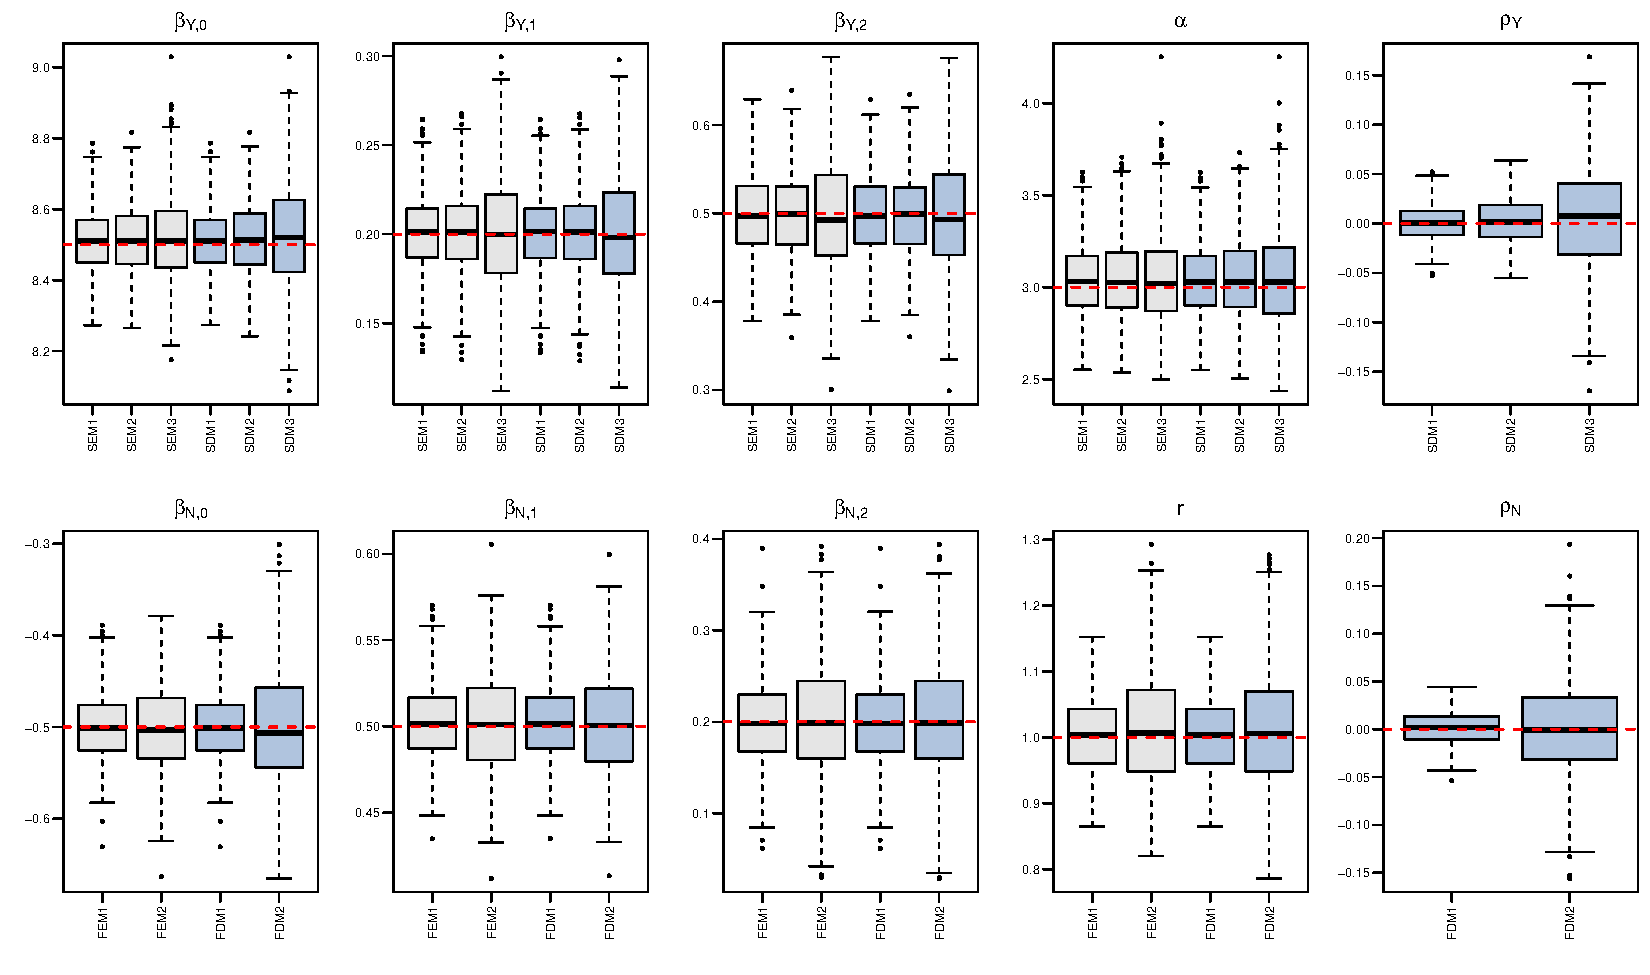
\includegraphics[width=1\linewidth]{Case1_Parameter_Boxplots.pdf}
    \caption{{Estimates of the severity and frequency parameters in Case 1}}
    \label{fig:simcase1}
\end{figure}

\begin{table}[h!]
\footnotesize
\centering
%{\color{blue}
\resizebox{\textwidth}{!}{%
    \begin{minipage}{0.65\textwidth}
        \centering
        \begin{tabular}{lcccccc}
        \toprule
        & \multicolumn{2}{c}{SEM1} & \multicolumn{2}{c}{SEM2} & \multicolumn{2}{c}{SEM3} \\
        \cmidrule(lr){2-3} \cmidrule(lr){4-5} \cmidrule(lr){6-7}
        & Mean & RMSE & Mean & RMSE & Mean & RMSE \\
        & (s.e.) & (Bias) & (s.e.) & (Bias) & (s.e.) & (Bias) \\
        \midrule
        \multirow{6}{*}{$\beta_Y$} & 8.5143 & 0.0898 & 8.5156 & 0.0979 & 8.5160 & 0.1312 \\
         & (0.0040) & (0.0143) & (0.0043) & (0.0156) & (0.0058) & (0.0160) \\
        \cmidrule{2-7}
         & 0.2007 & 0.0217 & 0.2007 & 0.0230 & 0.1999 & 0.0319 \\
         & (0.0010) & (0.0007) & (0.0010) & (0.0007) & (0.0014) & (-0.0001) \\
        \cmidrule{2-7}
         & 0.4991 & 0.0434 & 0.4986 & 0.0467 & 0.4959 & 0.0649 \\
         & (0.0019) & (-0.0009) & (0.0021) & (-0.0014) & (0.0029) & (-0.0041) \\
        \midrule
        \multirow{2}{*}{$\alpha$} & 3.0393 & 0.2027 & 3.0426 & 0.2173 & 3.0455 & 0.2564 \\
         & (0.0089) & (0.0393) & (0.0095) & (0.0426) & (0.0113) & (0.0455) \\
        \hhline{=======}
        \end{tabular}
    \end{minipage}
    \hspace{0.01\textwidth}
    \begin{minipage}{0.5\textwidth}
        \centering
        \begin{tabular}{lcccc}
        \toprule
        & \multicolumn{2}{c}{FEM1}  & \multicolumn{2}{c}{FEM2} \\
        \cmidrule(lr){2-3} \cmidrule(lr){4-5} 
        & Mean & RMSE & Mean & RMSE  \\
        & (s.e.) & (Bias)  & (s.e.) & (Bias) \\
        \midrule
        \multirow{6}{*}{$\beta_N$} & -0.5010 & 0.0350 & -0.5012 & 0.0497 \\
         & (0.0016) & (-0.0010) & (0.0022) & (-0.0012) \\
        \cmidrule{2-5}
         & 0.5017 & 0.0211 & 0.5017 & 0.0288 \\
         & (0.0009) & (0.0017) & (0.0013) & (0.0017) \\
        \cmidrule{2-5}
         & 0.1994 & 0.0453 & 0.2004 & 0.0610 \\
         & (0.0020) & (-0.0006) & (0.0027) & (0.0004) \\
        \midrule
        \multirow{2}{*}{$r$} & 1.0050 & 0.0580 & 1.0121 & 0.0844 \\
         & (0.0026) & (0.0050) & (0.0037) & (0.0121) \\
        \hhline{=====}
        \end{tabular}
    \end{minipage}
}
%}
\caption{Simulation result of SEM and FEM in Case 1}\label{tab:AppSimExoCase1}
\end{table}

\begin{table}[h!]
\footnotesize
\centering
%{\color{blue}
\resizebox{\textwidth}{!}{%
    \begin{minipage}{0.65\textwidth}
        \centering
        \begin{tabular}{lcccccc}
        \toprule
        & \multicolumn{2}{c}{SDM1} & \multicolumn{2}{c}{SDM2} & \multicolumn{2}{c}{SDM3} \\
        \cmidrule(lr){2-3} \cmidrule(lr){4-5} \cmidrule(lr){6-7}
        & Mean & RMSE & Mean & RMSE & Mean & RMSE \\
        & (s.e.) & (Bias) & (s.e.) & (Bias) & (s.e.) & (Bias) \\
        \midrule
        \multirow{6}{*}{$\beta_Y$} & 8.5143 & 0.0898 & 8.5181 & 0.1012 & 8.5225 & 0.1545 \\
         & (0.0040) & (0.0143) & (0.0045) & (0.0181) & (0.0068) & (0.0225) \\
        \cmidrule{2-7}
         & 0.2007 & 0.0217 & 0.2008 & 0.0230 & 0.2003 & 0.0319 \\
         & (0.0010) & (0.0007) & (0.0010) & (0.0008) & (0.0014) & (0.0003) \\
        \cmidrule{2-7}
         & 0.4991 & 0.0434 & 0.4985 & 0.0467 & 0.4962 & 0.0650 \\
         & (0.0019) & (-0.0009) & (0.0021) & (-0.0015) & (0.0029) & (-0.0038) \\
        \midrule
        \multirow{2}{*}{$\alpha$} & 3.0393 & 0.2027 & 3.0476 & 0.2236 & 3.0543 & 0.2812 \\
         & (0.0089) & (0.0393) & (0.0098) & (0.0476) & (0.0124) & (0.0543) \\
        \midrule
        \multirow{2}{*}{$\rho_Y$} & 0.0010 & 0.0178 & 0.0023 & 0.0230 & 0.0048 & 0.0539 \\
         & (0.0008) & (0.0010) & (0.0010) & (0.0023) & (0.0024) & (0.0048) \\
        \hhline{=======}
        \end{tabular}
    \end{minipage}
    \hspace{0.01\textwidth}
    \begin{minipage}{0.5\textwidth}
        \centering
        \begin{tabular}{lcccc}
        \toprule
        & \multicolumn{2}{c}{FDM1} & \multicolumn{2}{c}{FDM2} \\
        \cmidrule(lr){2-3} \cmidrule(lr){4-5}
        & Mean & RMSE & Mean & RMSE \\
        & (s.e.) & (Bias) & (s.e.) & (Bias) \\
        \midrule
        \multirow{6}{*}{$\beta_N$} & -0.5010 & 0.0350 & -0.5009 & 0.0637 \\
         & (0.0016) & (-0.0010) & (0.0029) & (-0.0009) \\
        \cmidrule{2-5}
         & 0.5017 & 0.0211 & 0.5011 & 0.0287 \\
         & (0.0009) & (0.0017) & (0.0013) & (0.0011) \\
        \cmidrule{2-5}
         & 0.1994 & 0.0453 & 0.2001 & 0.0610 \\
         & (0.0020) & (-0.0006) & (0.0027) & (0.0001) \\
        \midrule
        \multirow{2}{*}{$r$} & 1.0050 & 0.0580 & 1.0107 & 0.0867 \\
         & (0.0026) & (0.0050) & (0.0039) & (0.0107) \\
        \midrule
        \multirow{2}{*}{$\rho_N$} & 0.0014 & 0.0181 & 0.0012 & 0.0517 \\
         & (0.0008) & (0.0014) & (0.0023) & (0.0012) \\
        \hhline{=====}
        \end{tabular}
    \end{minipage}
}
%}
\caption{Simulation result of SDM and FDM in Case 1}\label{tab:AppSimEndCase1}
\end{table}

\begin{figure}[h!]
    \centering
    \includegraphics[width=1\linewidth]{Case2_Parameter_Boxplots.pdf}
    \caption{{Estimates of the severity and frequency parameters in Case 2}}
    \label{fig:simcase2}
\end{figure}

\begin{table}[h!]
\footnotesize
\centering
%{\color{blue}
%\resizebox{\textwidth}{!}{
        \begin{tabular}{lcccccc}
        \toprule
        & \multicolumn{2}{c}{SEM1} & \multicolumn{2}{c}{SEM2} & \multicolumn{2}{c}{SEM3} \\
        \cmidrule(lr){2-3} \cmidrule(lr){4-5} \cmidrule(lr){6-7}
        & Mean & RMSE & Mean & RMSE & Mean & RMSE \\
        & (s.e.) & (Bias) & (s.e.) & (Bias) & (s.e.) & (Bias) \\
        \midrule
        \multirow{6}{*}{$\beta_Y$} & 8.4997 & 0.0905 & 8.4993 & 0.0942 & 8.4989 & 0.1188 \\
         & (0.0041) & (-0.0003) & (0.0042) & (-0.0007) & (0.0053) & (-0.0011) \\
        \cmidrule{2-7}
         & 0.1995 & 0.0216 & 0.1998 & 0.0220 & 0.2003 & 0.0283 \\
         & (0.0010) & (-0.0005) & (0.0010) & (-0.0002) & (0.0013) & (0.0003) \\
        \cmidrule{2-7}
         & 0.5010 & 0.0424 & 0.5016 & 0.0431 & 0.5022 & 0.0579 \\
         & (0.0019) & (0.0010) & (0.0019) & (0.0016) & (0.0026) & (0.0022) \\
        \midrule
        \multirow{2}{*}{$\alpha$} & 3.0115 & 0.2002 & 3.0123 & 0.2069 & 3.0159 & 0.2326 \\
         & (0.0089) & (0.0115) & (0.0092) & (0.0123) & (0.0104) & (0.0159) \\
        \hhline{=======}
        \end{tabular}
%}
%}
\caption{Simulation result of SEM in Case 2}\label{tab:AppSimExoCase2}
\end{table}

\begin{table}[h!]
\footnotesize
\centering
%{\color{blue}
\resizebox{\textwidth}{!}{%
    \begin{minipage}[t]{0.5\textwidth}
    \vspace{0pt}
    \centering
        \begin{tabular}{lcccc}
        \toprule
        & \multicolumn{2}{c}{FEM1}  & \multicolumn{2}{c}{FEM2} \\
        \cmidrule(lr){2-3} \cmidrule(lr){4-5} 
        & Mean & RMSE & Mean & RMSE\\
        & (s.e.) & (Bias) & (s.e.) & (Bias) \\
        \midrule
        \multirow{6}{*}{$\beta_N$} & -0.5035 & 0.0361 & -0.3274 & 0.1782 \\
         & (0.0016) & (-0.0035) & (0.0020) & (0.1726) \\
        \cmidrule{2-5}
         & 0.5004 & 0.0230 & 0.5031 & 0.0262 \\
         & (0.0010) & (0.0004) & (0.0012) & (0.0031) \\
        \cmidrule{2-5}
         & 0.2041 & 0.0424 & 0.1941 & 0.0516 \\
         & (0.0019) & (0.0041) & (0.0023) & (-0.0059) \\
        \midrule
        \multirow{2}{*}{$r$} & 1.0057 & 0.0566 & 1.4723 & 0.4893 \\
         & (0.0025) & (0.0057) & (0.0057) & (0.4723) \\
        \hhline{=====}
        \end{tabular}
    \end{minipage}
    \hspace{0.01\textwidth}
    \begin{minipage}[t]{0.5\textwidth}
    \vspace{0pt}
    \centering
        \begin{tabular}{lcccc}
        \toprule
        & \multicolumn{2}{c}{FDM1} & \multicolumn{2}{c}{FDM2} \\
        \cmidrule(lr){2-3} \cmidrule(lr){4-5}
        & Mean & RMSE & Mean & RMSE \\
        & (s.e.) & (Bias) & (s.e.) & (Bias) \\
        \midrule
        \multirow{6}{*}{$\beta_N$} & -0.5034 & 0.0359 & -0.5016 & 0.0453 \\
 & (0.0016) & (-0.0034) & (0.0020) & (-0.0016) \\
        \cmidrule{2-5}
         & 0.5003 & 0.0229 & 0.4996 & 0.0266 \\
 & (0.0010) & (0.0003) & (0.0012) & (-0.0004) \\
        \cmidrule{2-5}
         & 0.2044 & 0.0420 & 0.2026 & 0.0515 \\
 & (0.0019) & (0.0044) & (0.0023) & (0.0026) \\
        \midrule
        \multirow{2}{*}{$r$} & 1.0051 & 0.0554 & 1.0030 & 0.0877 \\
 & (0.0025) & (0.0051) & (0.0039) & (0.0030) \\
        \midrule
        \multirow{2}{*}{$\rho_N$} & -0.4992 & 0.0152 & -0.4994 & 0.0324 \\
 & (0.0007) & (0.0008) & (0.0015) & (0.0006) \\
        \hhline{=====}
        \end{tabular}
    \end{minipage}
}
%}
\caption{Simulation result of FEM and FDM in Case 2}\label{tab:AppSimEndCase2}
\end{table}

\begin{figure}[h!]
    \centering
    \includegraphics[width=1\linewidth]{Case3_Parameter_Boxplots.pdf}
    \caption{{Estimates of the severity and frequency parameters in Case 3}}
    \label{fig:simcase3}
\end{figure}

\begin{table}[h!]
\footnotesize
\centering
%{\color{blue}
\resizebox{\textwidth}{!}{%
    \begin{minipage}{0.65\textwidth}
        \centering
        \begin{tabular}{lcccccc}
        \toprule
        & \multicolumn{2}{c}{SEM1} & \multicolumn{2}{c}{SEM2} & \multicolumn{2}{c}{SEM3} \\
        \cmidrule(lr){2-3} \cmidrule(lr){4-5} \cmidrule(lr){6-7}
        & Mean & RMSE & Mean & RMSE & Mean & RMSE \\
        & (s.e.) & (Bias) & (s.e.) & (Bias) & (s.e.) & (Bias) \\
        \midrule
        \multirow{6}{*}{$\beta_Y$} & 8.5082 & 0.0938 & 9.0514 & 0.5624 & 9.1764 & 0.6919 \\
        & (0.0042) & (0.0082) & (0.0050) & (0.5514) & (0.0065) & (0.6764) \\
        \cmidrule{2-7}
         & 0.2016 & 0.0256 & 0.2081 & 0.0247 & 0.2424 & 0.0517 \\
         & (0.0011) & (0.0016) & (0.0010) & (0.0081) & (0.0013) & (0.0424) \\
        \cmidrule{2-7}
         & 0.4985 & 0.0513 & 0.4812 & 0.0503 & 0.5230 & 0.0629 \\
         & (0.0023) & (-0.0015) & (0.0021) & (-0.0188) & (0.0026) & (0.0230) \\
        \midrule
        \multirow{2}{*}{$\alpha$} & 3.0272 & 0.2047 & 4.3039 & 1.3621 & 4.4034 & 1.4894 \\
         & (0.0091) & (0.0272) & (0.0177) & (1.3039) & (0.0224) & (1.4034) \\
        \hhline{=======}
        \end{tabular}
    \end{minipage}
    \hspace{0.01\textwidth}
    \begin{minipage}{0.65\textwidth}
        \centering
        \begin{tabular}{lcccccc}
        \toprule
        & \multicolumn{2}{c}{FEM1} & \multicolumn{2}{c}{FEM2G} & \multicolumn{2}{c}{FEM2} \\
        \cmidrule(lr){2-3} \cmidrule(lr){4-5} \cmidrule(lr){6-7}
        & Mean & RMSE & Mean & RMSE & Mean & RMSE \\
        & (s.e.) & (Bias) & (s.e.) & (Bias) & (s.e.) & (Bias) \\
        \midrule
        \multirow{6}{*}{$\beta_N$} & -0.5020 & 0.0379 & -0.5005 & 0.0895 & -0.5840 & 0.0980 \\
 & (0.0017) & (-0.0020) & (0.0040) & (-0.0005) & (0.0023) & (-0.0840) \\
        \cmidrule{2-7}
         & 0.5008 & 0.0230 & 0.5007 & 0.0320 & 0.4578 & 0.0517 \\
 & (0.0010) & (0.0008) & (0.0014) & (0.0007) & (0.0013) & (-0.0422) \\
        \cmidrule{2-7}
         & 0.2006 & 0.0463 & 0.1972 & 0.0946 & 0.1607 & 0.0730 \\
 & (0.0021) & (0.0006) & (0.0042) & (-0.0028) & (0.0028) & (-0.0393) \\
        \midrule
        \multirow{2}{*}{$r$} & 1.0061 & 0.0588 & 1.0072 & 0.0958 & 0.9004 & 0.1235 \\
 & (0.0026) & (0.0061) & (0.0043) & (0.0072) & (0.0033) & (-0.0996) \\
        \hhline{=======}
        \end{tabular}
    \end{minipage}
}
%}
\caption{Simulation result of SEM and FEM in Case 3}\label{tab:AppSimExoCase3}
\end{table}

\begin{table}[h!]
\footnotesize
\centering
%{\color{blue}
%\resizebox{\textwidth}{!}{%
    \begin{minipage}{0.65\textwidth}
        \centering
        \begin{tabular}{lcccccc}
        \toprule
        & \multicolumn{2}{c}{SDM1} & \multicolumn{2}{c}{SDM2} & \multicolumn{2}{c}{SDM3} \\
        \cmidrule(lr){2-3} \cmidrule(lr){4-5} \cmidrule(lr){6-7}
        & Mean & RMSE & Mean & RMSE & Mean & RMSE \\
        & (s.e.) & (Bias) & (s.e.) & (Bias) & (s.e.) & (Bias) \\
        \midrule
        \multirow{6}{*}{$\beta_Y$} & 8.4985 & 0.0885 & 8.4989 & 0.1025 & 8.5084 & 0.1258 \\
         & (0.0040) & (-0.0015) & (0.0046) & (-0.0011) & (0.0056) & (0.0084) \\
        \cmidrule{2-7}
         & 0.1998 & 0.0198 & 0.1993 & 0.0212 & 0.1982 & 0.0273 \\
         & (0.0009) & (-0.0002) & (0.0009) & (-0.0007) & (0.0012) & (-0.0018) \\
        \cmidrule{2-7}
         & 0.5008 & 0.0422 & 0.5008 & 0.0452 & 0.4970 & 0.0562 \\
         & (0.0019) & (0.0008) & (0.0020) & (0.0008) & (0.0025) & (-0.0030) \\
        \midrule
        \multirow{2}{*}{$\alpha$} & 3.0065 & 0.1964 & 3.0090 & 0.2200 & 3.0244 & 0.2588 \\
         & (0.0088) & (0.0065) & (0.0098) & (0.0090) & (0.0115) & (0.0244) \\
        \midrule
        \multirow{2}{*}{$\rho_Y$} & -0.5005 & 0.0126 & -0.5008 & 0.0176 & -0.4998 & 0.0283 \\
         & (0.0006) & (-0.0005) & (0.0008) & (-0.0008) & (0.0013) & (0.0002) \\
        \hhline{=======}
        \end{tabular}
    \end{minipage}
%}
%}
\caption{Simulation result of SDM in Case 3}\label{tab:AppSimEndCase3}
\end{table}

\begin{figure}[h!]
    \centering
    \includegraphics[width=1\linewidth]{Case4_Parameter_Boxplots.pdf}
    \caption{{Estimates of the severity and frequency parameters in Case 4}}
    \label{fig:simcase4}
\end{figure}

\begin{table}[h!]
\footnotesize
\centering
%{\color{blue}
\resizebox{\textwidth}{!}{%
    \begin{minipage}{0.65\textwidth}
        \centering
        \begin{tabular}{lcccccc}
        \toprule
        & \multicolumn{2}{c}{SEM1} & \multicolumn{2}{c}{SEM2} & \multicolumn{2}{c}{SEM3} \\
        \cmidrule(lr){2-3} \cmidrule(lr){4-5} \cmidrule(lr){6-7}
        & Mean & RMSE & Mean & RMSE & Mean & RMSE \\
        & (s.e.) & (Bias) & (s.e.) & (Bias) & (s.e.) & (Bias) \\
        \midrule
        \multirow{6}{*}{$\beta_Y$} & 9.0116 & 0.5205 & 9.1002 & 0.6088 & 9.0374 & 0.5510 \\
        & (0.0043) & (0.5116) & (0.0046) & (0.6002) & (0.0055) & (0.5374) \\
        \cmidrule{2-7}
         & 0.2107 & 0.0239 & 0.2185 & 0.0277 & 0.2465 & 0.0524 \\
         & (0.0010) & (0.0107) & (0.0009) & (0.0185) & (0.0011) & (0.0465) \\
        \cmidrule{2-7}
         & 0.5278 & 0.0520 & 0.5283 & 0.0519 & 0.5531 & 0.0733 \\
         & (0.0020) & (0.0278) & (0.0019) & (0.0283) & (0.0023) & (0.0531) \\
        \midrule
        \multirow{2}{*}{$\alpha$} & 3.7620 & 0.8146 & 4.0100 & 1.0624 & 3.8464 & 0.9141 \\
        & (0.0129) & (0.7620) & (0.0148) & (1.0100) & (0.0155) & (0.8464) \\
        \hhline{=======}
        \end{tabular}
    \end{minipage}
    \hspace{0.01\textwidth}
    \begin{minipage}{0.5\textwidth}
        \centering
        \begin{tabular}{lcccc}
        \toprule
        & \multicolumn{2}{c}{FEM1}  & \multicolumn{2}{c}{FEM2} \\
        \cmidrule(lr){2-3} \cmidrule(lr){4-5} 
        & Mean & RMSE & Mean & RMSE \\
        & (s.e.) & (Bias)  & (s.e.) & (Bias) \\
        \midrule
        \multirow{6}{*}{$\beta_N$} & -0.5016 & 0.0353 & -0.3185 & 0.1862 \\
        & (0.0016) & (-0.0016) & (0.0019) & (0.1815) \\
        \cmidrule{2-5}
         & 0.5008 & 0.0233 & 0.4743 & 0.0360 \\
        & (0.0010) & (0.0008) & (0.0011) & (-0.0257) \\
        \cmidrule{2-5}
         & 0.2007 & 0.0450 & 0.1633 & 0.0616 \\
        & (0.0020) & (0.0007) & (0.0022) & (-0.0367) \\
        \midrule
        \multirow{2}{*}{$r$} & 1.0048 & 0.0598 & 1.3070 & 0.3249 \\
         & (0.0027) & (0.0048) & (0.0048) & (0.3070) \\
        \hhline{=====}
        \end{tabular}
    \end{minipage}
}
%}
\caption{Simulation result of SEM and FEM in Case 4}\label{tab:AppSimExoCase4}
\end{table}

\begin{table}[h!]
\footnotesize
\centering
%{\color{blue}
\resizebox{\textwidth}{!}{%
    \begin{minipage}{0.65\textwidth}
        \centering
        \begin{tabular}{lcccccc}
        \toprule
        & \multicolumn{2}{c}{SDM1} & \multicolumn{2}{c}{SDM2} & \multicolumn{2}{c}{SDM3} \\
        \cmidrule(lr){2-3} \cmidrule(lr){4-5} \cmidrule(lr){6-7}
        & Mean & RMSE & Mean & RMSE & Mean & RMSE \\
        & (s.e.) & (Bias) & (s.e.) & (Bias) & (s.e.) & (Bias) \\
        \midrule
        \multirow{6}{*}{$\beta_Y$} & 8.5062 & 0.0860 & 8.5050 & 0.0938 & 8.5071 & 0.1166 \\
 & (0.0038) & (0.0062) & (0.0042) & (0.0050) & (0.0052) & (0.0071) \\
        \cmidrule{2-7}
         & 0.2001 & 0.0195 & 0.2001 & 0.0199 & 0.2003 & 0.0238 \\
 & (0.0009) & (0.0001) & (0.0009) & (0.0001) & (0.0011) & (0.0003) \\
        \cmidrule{2-7}
         & 0.5048 & 0.0432 & 0.5051 & 0.0440 & 0.5050 & 0.0494 \\
 & (0.0019) & (0.0048) & (0.0020) & (0.0051) & (0.0022) & (0.0050) \\
        \midrule
        \multirow{2}{*}{$\alpha$} & 3.0295 & 0.1831 & 3.0287 & 0.1921 & 3.0345 & 0.2224 \\
 & (0.0081) & (0.0295) & (0.0085) & (0.0287) & (0.0098) & (0.0345) \\
        \midrule
        \multirow{2}{*}{$\rho_Y$} & -0.4003 & 0.0176 & -0.4008 & 0.0206 & -0.3995 & 0.0325 \\
 & (0.0008) & (-0.0003) & (0.0009) & (-0.0008) & (0.0015) & (0.0005) \\
        \hhline{=======}
        \end{tabular}
    \end{minipage}
    \hspace{0.01\textwidth}
    \begin{minipage}{0.5\textwidth}
        \centering
        \begin{tabular}{lcccc}
        \toprule
        & \multicolumn{2}{c}{FDM1} & \multicolumn{2}{c}{FDM2} \\
        \cmidrule(lr){2-3} \cmidrule(lr){4-5}
        & Mean & RMSE & Mean & RMSE \\
        & (s.e.) & (Bias) & (s.e.) & (Bias) \\
        \midrule
        \multirow{6}{*}{$\beta_N$} & -0.5026 & 0.0392 & -0.5024 & 0.0479 \\
         & (0.0017) & (-0.0026) & (0.0021) & (-0.0024) \\
        \cmidrule{2-5}
         & 0.5013 & 0.0224 & 0.5014 & 0.0266 \\
         & (0.0010) & (0.0013) & (0.0012) & (0.0014) \\
        \cmidrule{2-5}
         & 0.2030 & 0.0482 & 0.2030 & 0.0560 \\
         & (0.0022) & (0.0030) & (0.0025) & (0.0030) \\
        \midrule
        \multirow{2}{*}{$r$} & 1.0035 & 0.0575 & 1.0057 & 0.0829 \\
         & (0.0026) & (0.0035) & (0.0037) & (0.0057) \\
        \midrule
        \multirow{2}{*}{$\rho_N$} & -0.6014 & 0.0135 & -0.6008 & 0.0251 \\
         & (0.0006) & (-0.0014) & (0.0011) & (-0.0008) \\
        \hhline{=====}
        \end{tabular}
    \end{minipage}
}
%}
\caption{Simulation result of SDM and FDM in Case 4}\label{tab:AppSimEndCase4}
\end{table}

% \begin{table}[!ht]
% \footnotesize
% \centering
% {\color{blue}
% \resizebox{\textwidth}{!}{%
%     \begin{minipage}{0.65\textwidth}
%         \centering
%         \begin{tabular}{lcccccc}
%         \toprule
%         & \multicolumn{2}{c}{SEM1} & \multicolumn{2}{c}{SEM2} & \multicolumn{2}{c}{SEM3} \\
%         \cmidrule(lr){2-3} \cmidrule(lr){4-5} \cmidrule(lr){6-7}
%         & Mean & RMSE & Mean & RMSE & Mean & RMSE \\
%         & (s.e.) & (Bias) & (s.e.) & (Bias) & (s.e.) & (Bias) \\
%         \midrule
%         \multirow{6}{*}{$\beta_Y$} & 9.0879 & 0.5958 & 9.1729 & 0.6802 & 9.1212 & 0.6322 \\
%          & (0.0043) & (0.5879) & (0.0044) & (0.6729) & (0.0052) & (0.6212) \\
%         \cmidrule{2-7}
%          & 0.1683 & 0.0394 & 0.1754 & 0.0336 & 0.2060 & 0.0274 \\
%          & (0.0010) & (-0.0317) & (0.0010) & (-0.0246) & (0.0012) & (0.0060) \\
%         \cmidrule{2-7}
%          & 0.4875 & 0.0508 & 0.4864 & 0.0503 & 0.5171 & 0.0604 \\
%          & (0.0022) & (-0.0125) & (0.0022) & (-0.0136) & (0.0026) & (0.0171) \\
%         \midrule
%         \multirow{2}{*}{$\alpha$} & 3.5715 & 0.6314 & 3.7904 & 0.8449 & 3.6719 & 0.7422 \\
%          & (0.0120) & (0.5715) & (0.0134) & (0.7904) & (0.0141) & (0.6719) \\
%         \hhline{=======}
%         \end{tabular}
%     \end{minipage}
%     \hspace{0.01\textwidth}
%     \begin{minipage}{0.65\textwidth}
%         \centering
%         \begin{tabular}{lcccccc}
%         \toprule
%         & \multicolumn{2}{c}{FEM1} & \multicolumn{2}{c}{FEM2G} & \multicolumn{2}{c}{FEM2} \\
%         \cmidrule(lr){2-3} \cmidrule(lr){4-5} \cmidrule(lr){6-7}
%         & Mean & RMSE & Mean & RMSE & Mean & RMSE \\
%         & (s.e.) & (Bias) & (s.e.) & (Bias) & (s.e.) & (Bias) \\
%         \midrule
%         \multirow{6}{*}{$\beta_N$} & -0.5014 & 0.0373 & -0.3308 & 0.1734 & -0.3329 & 0.1722 \\
%          & (0.0017) & (-0.0014) & (0.0017) & (0.1692) & (0.0019) & (0.1671) \\
%         \cmidrule{2-7}
%          & 0.5006 & 0.0236 & 0.4856 & 0.0270 & 0.4732 & 0.0365 \\
%          & (0.0011) & (0.0006) & (0.0010) & (-0.0144) & (0.0011) & (-0.0268) \\
%         \cmidrule{2-7}
%          & 0.1997 & 0.0451 & 0.1691 & 0.0541 & 0.1608 & 0.0624 \\
%          & (0.0020) & (-0.0003) & (0.0020) & (-0.0309) & (0.0022) & (-0.0392) \\
%         \midrule
%         \multirow{2}{*}{$r$} & 1.0070 & 0.0607 & 1.2262 & 0.2455 & 1.2000 & 0.2209 \\
%          & (0.0027) & (0.0070) & (0.0043) & (0.2262) & (0.0042) & (0.2000) \\
%         \hhline{=======}
%         \end{tabular}
%     \end{minipage}
% }
% }
% \caption{Simulation result of SEM and FEM in Case 5 (discrete deductible)}\label{tab:AppSimExoCase5}
% \end{table}

% \begin{table}[!ht]
% \footnotesize
% \centering
% {\color{blue}
% \resizebox{\textwidth}{!}{%
%     \begin{minipage}{0.65\textwidth}
%         \centering
%         \begin{tabular}{lcccccc}
%         \toprule
%         & \multicolumn{2}{c}{SDM1} & \multicolumn{2}{c}{SDM2} & \multicolumn{2}{c}{SDM3} \\
%         \cmidrule(lr){2-3} \cmidrule(lr){4-5} \cmidrule(lr){6-7}
%         & Mean & RMSE & Mean & RMSE & Mean & RMSE \\
%         & (s.e.) & (Bias) & (s.e.) & (Bias) & (s.e.) & (Bias) \\
%         \midrule
%         \multirow{6}{*}{$\beta_Y$} & 8.5574 & 0.1041 & 8.5396 & 0.0993 & 8.5367 & 0.1190 \\
%          & (0.0039) & (0.0574) & (0.0041) & (0.0396) & (0.0051) & (0.0367) \\
%         \cmidrule{2-7}
%          & 0.1576 & 0.0479 & 0.1550 & 0.0503 & 0.1547 & 0.0523 \\
%          & (0.0010) & (-0.0424) & (0.0010) & (-0.0450) & (0.0012) & (-0.0453) \\
%         \cmidrule{2-7}
%          & 0.4618 & 0.0600 & 0.4586 & 0.0626 & 0.4605 & 0.0677 \\
%          & (0.0021) & (-0.0382) & (0.0021) & (-0.0414) & (0.0025) & (-0.0395) \\
%         \midrule
%         \multirow{2}{*}{$\alpha$} & 2.8691 & 0.2118 & 2.8367 & 0.2357 & 2.8393 & 0.2546 \\
%          & (0.0074) & (-0.1309) & (0.0076) & (-0.1633) & (0.0088) & (-0.1607) \\
%         \midrule
%         \multirow{2}{*}{$\rho_Y$} & -0.4276 & 0.0327 & -0.4351 & 0.0405 & -0.4414 & 0.0527 \\
%          & (0.0008) & (-0.0276) & (0.0009) & (-0.0351) & (0.0015) & (-0.0414) \\
%         \hhline{=======}
%         \end{tabular}
%     \end{minipage}
%     \hspace{0.01\textwidth}
%     \begin{minipage}{0.5\textwidth}
%         \centering
%         \begin{tabular}{lcccc}
%         \toprule
%         & \multicolumn{2}{c}{FDM1} & \multicolumn{2}{c}{FDM2} \\
%         \cmidrule(lr){2-3} \cmidrule(lr){4-5}
%         & Mean & RMSE & Mean & RMSE \\
%         & (s.e.) & (Bias) & (s.e.) & (Bias) \\
%         \midrule
%         \multirow{6}{*}{$\beta_N$} & -0.5011 & 0.0371 & -0.5024 & 0.0452 \\
%          & (0.0017) & (-0.0011) & (0.0020) & (-0.0024) \\
%         \cmidrule{2-5}
%          & 0.5005 & 0.0225 & 0.5000 & 0.0256 \\
%          & (0.0010) & (0.0005) & (0.0011) & (-0.0000) \\
%         \cmidrule{2-5}
%          & 0.1991 & 0.0451 & 0.1986 & 0.0527 \\
%          & (0.0020) & (-0.0009) & (0.0024) & (-0.0014) \\
%         \midrule
%         \multirow{2}{*}{$r$} & 1.0080 & 0.0601 & 0.9606 & 0.0883 \\
%          & (0.0027) & (0.0080) & (0.0035) & (-0.0394) \\
%         \midrule
%         \multirow{2}{*}{$\rho_N$} & -0.6001 & 0.0129 & -0.5981 & 0.0249 \\
%          & (0.0006) & (-0.0001) & (0.0011) & (0.0019) \\
%         \hhline{=====}
%         \end{tabular}
%     \end{minipage}
% }
% }
% \caption{Simulation result of SDM and FDM in Case 5 (discrete deductible)}\label{tab:AppSimEndCase5}
% \end{table}

% \begin{table}[!ht]
% \footnotesize
% \centering
% {\color{blue}
% \resizebox{\textwidth}{!}{%
%     \begin{minipage}{0.65\textwidth}
%         \centering
%         \begin{tabular}{lcccccc}
%         \toprule
%         & \multicolumn{2}{c}{SEM1} & \multicolumn{2}{c}{SEM2} & \multicolumn{2}{c}{SEM3} \\
%         \cmidrule(lr){2-3} \cmidrule(lr){4-5} \cmidrule(lr){6-7}
%         & Mean & RMSE & Mean & RMSE & Mean & RMSE \\
%         & (s.e.) & (Bias) & (s.e.) & (Bias) & (s.e.) & (Bias) \\
%         \midrule
%         \multirow{6}{*}{$\beta_Y$} & 9.6677 & 1.1727 & 9.6888 & 1.1940 & 9.5161 & 1.0225 \\
%          & (0.0049) & (1.1677) & (0.0050) & (1.1888) & (0.0051) & (1.0161) \\
%         \cmidrule{2-7}
%          & 0.1450 & 0.0603 & 0.1480 & 0.0576 & 0.1789 & 0.0351 \\
%          & (0.0011) & (-0.0550) & (0.0011) & (-0.0520) & (0.0013) & (-0.0211) \\
%         \cmidrule{2-7}
%          & 0.4756 & 0.0549 & 0.4750 & 0.0552 & 0.5038 & 0.0543 \\
%          & (0.0022) & (-0.0244) & (0.0022) & (-0.0250) & (0.0024) & (0.0038) \\
%         \midrule
%         \multirow{2}{*}{$\alpha$} & 4.4549 & 1.5126 & 4.5238 & 1.5831 & 4.0805 & 1.1433 \\
%          & (0.0185) & (1.4549) & (0.0192) & (1.5238) & (0.0167) & (1.0805) \\
%         \hhline{=======}
%         \end{tabular}
%     \end{minipage}
%     \hspace{0.01\textwidth}
%     \begin{minipage}{0.65\textwidth}
%         \centering
%         \begin{tabular}{lcccccc}
%         \toprule
%         & \multicolumn{2}{c}{FEM1} & \multicolumn{2}{c}{FEM2G} & \multicolumn{2}{c}{FEM2} \\
%         \cmidrule(lr){2-3} \cmidrule(lr){4-5} \cmidrule(lr){6-7}
%         & Mean & RMSE & Mean & RMSE & Mean & RMSE \\
%         & (s.e.) & (Bias) & (s.e.) & (Bias) & (s.e.) & (Bias) \\
%         \midrule
%         \multirow{6}{*}{$\beta_N$} & -0.5032 & 0.0372 & -0.3452 & 0.1589 & -0.3309 & 0.1731 \\
%          & (0.0017) & (-0.0032) & (0.0016) & (0.1548) & (0.0017) & (0.1691) \\
%         \cmidrule{2-7}
%          & 0.4995 & 0.0230 & 0.4797 & 0.0304 & 0.4717 & 0.0369 \\
%          & (0.0010) & (-0.0005) & (0.0010) & (-0.0203) & (0.0011) & (-0.0283) \\
%         \cmidrule{2-7}
%          & 0.2023 & 0.0450 & 0.1700 & 0.0526 & 0.1619 & 0.0589 \\
%          & (0.0020) & (0.0023) & (0.0019) & (-0.0300) & (0.0020) & (-0.0381) \\
%         \midrule
%         \multirow{2}{*}{$r$} & 1.0055 & 0.0606 & 1.0846 & 0.1130 & 1.0877 & 0.1163 \\
%          & (0.0027) & (0.0055) & (0.0033) & (0.0846) & (0.0034) & (0.0877) \\
%         \hhline{=======}
%         \end{tabular}
%     \end{minipage}
% }
% }
% \caption{Simulation result of SEM and FEM in Case 6 (discrete deductible)}\label{tab:AppSimExoCase6}
% \end{table}

% \begin{table}[!ht]
% \footnotesize
% \centering
% {\color{blue}
% \resizebox{\textwidth}{!}{%
%     \begin{minipage}{0.65\textwidth}
%         \centering
%         \begin{tabular}{lcccccc}
%         \toprule
%         & \multicolumn{2}{c}{SDM1} & \multicolumn{2}{c}{SDM2} & \multicolumn{2}{c}{SDM3} \\
%         \cmidrule(lr){2-3} \cmidrule(lr){4-5} \cmidrule(lr){6-7}
%         & Mean & RMSE & Mean & RMSE & Mean & RMSE \\
%         & (s.e.) & (Bias) & (s.e.) & (Bias) & (s.e.) & (Bias) \\
%         \midrule
%         \multirow{6}{*}{$\beta_Y$} & 9.1478 & 0.6547 & 9.0805 & 0.5889 & 8.9253 & 0.4392 \\
%          & (0.0042) & (0.6478) & (0.0044) & (0.5805) & (0.0049) & (0.4253) \\
%         \cmidrule{2-7}
%          & 0.1337 & 0.0699 & 0.1298 & 0.0738 & 0.1331 & 0.0717 \\
%          & (0.0010) & (-0.0663) & (0.0010) & (-0.0702) & (0.0012) & (-0.0669) \\
%         \cmidrule{2-7}
%          & 0.4527 & 0.0659 & 0.4518 & 0.0675 & 0.4562 & 0.0679 \\
%          & (0.0020) & (-0.0473) & (0.0021) & (-0.0482) & (0.0023) & (-0.0438) \\
%         \midrule
%         \multirow{2}{*}{$\alpha$} & 3.5041 & 0.5614 & 3.3556 & 0.4285 & 3.0872 & 0.2432 \\
%          & (0.0110) & (0.5041) & (0.0107) & (0.3556) & (0.0102) & (0.0872) \\
%         \midrule
%         \multirow{2}{*}{$\rho_Y$} & -0.4144 & 0.0261 & -0.4245 & 0.0336 & -0.4332 & 0.0471 \\
%          & (0.0010) & (-0.0144) & (0.0010) & (-0.0245) & (0.0015) & (-0.0332) \\
%         \hhline{=======}
%         \end{tabular}
%     \end{minipage}
%     \hspace{0.01\textwidth}
%     \begin{minipage}{0.5\textwidth}
%         \centering
%         \begin{tabular}{lcccc}
%         \toprule
%         & \multicolumn{2}{c}{FDM1} & \multicolumn{2}{c}{FDM2} \\
%         \cmidrule(lr){2-3} \cmidrule(lr){4-5}
%         & Mean & RMSE & Mean & RMSE \\
%         & (s.e.) & (Bias) & (s.e.) & (Bias) \\
%         \midrule
%         \multirow{6}{*}{$\beta_N$} & -0.5031 & 0.0368 & -0.4605 & 0.0572 \\
%          & (0.0016) & (-0.0031) & (0.0018) & (0.0395) \\
%         \cmidrule{2-5}
%          & 0.4992 & 0.0221 & 0.4989 & 0.0253 \\
%          & (0.0010) & (-0.0008) & (0.0011) & (-0.0011) \\
%         \cmidrule{2-5}
%          & 0.2023 & 0.0440 & 0.1994 & 0.0485 \\
%          & (0.0020) & (0.0023) & (0.0022) & (-0.0006) \\
%         \midrule
%         \multirow{2}{*}{$r$} & 1.0058 & 0.0598 & 0.9258 & 0.1004 \\
%          & (0.0027) & (0.0058) & (0.0030) & (-0.0742) \\
%         \midrule
%         \multirow{2}{*}{$\rho_N$} & -0.6002 & 0.0138 & -0.5597 & 0.0465 \\
%          & (0.0006) & (-0.0002) & (0.0010) & (0.0403) \\
%         \hhline{=====}
%         \end{tabular}
%     \end{minipage}
% }
% }
% \caption{Simulation result of SDM and FDM in Case 6 (discrete deductible)}\label{tab:AppSimEndCase6}
% \end{table}

\FloatBarrier

\section{Deductible's distribution and estimation results for modeling}
\label{app:C}


\begin{table}[h!]
\centering
\resizebox{\ifdim\width>\linewidth\linewidth\else\width\fi}{!}{
\begin{tabular}{lrr@{\hspace{1.5cm}}lrr}
\toprule
\multicolumn{3}{c}{\textbf{Continuous deductible}}
&
\multicolumn{3}{c}{\textbf{Discrete deductible}} \\
\cmidrule(lr){1-3}
\cmidrule(lr){4-6}
Parameter & Estimate & s.e.
& Parameter & Estimate & s.e. \\
\midrule
(Intercept) & 5.858 & 0.118
& 1|2 & 1.283 & 0.120 \\
TypeCity & -2.296 & 0.076
& 2|3 & 2.320 & 0.124 \\
TypeCounty & -2.928 & 0.097
& 3|4 & 3.146 & 0.128 \\
TypeSchool & -2.089 & 0.069
& 4|5 & 4.451 & 0.138 \\
TypeTown & 0.582 & 0.074
& 5|6 & 5.117 & 0.146 \\
TypeVillage & -1.067 & 0.071
& 6|7 & 5.447 & 0.151 \\
$\sigma$ & 0.846 & 0.094
& 7|8 & 7.190 & 0.216 \\
$\alpha_1$ & 1.701 & 0.320
& 8|9 & 8.036 & 0.286 \\
$\alpha_2$ & 1.218 & 0.198
& 9|10 & 8.345 & 0.321 \\
& & & \multicolumn{3}{l}{} \\
& & & TypeCity & 1.339 & 0.146 \\
& & & TypeCounty & 1.828 & 0.183 \\
& & & TypeSchool & 0.852 & 0.136 \\
& & & TypeTown & -0.181 & 0.149 \\
& & & TypeVillage & 0.699 & 0.128 \\
& & & $\log(\mathrm{Coverage})$ & -0.967 & 0.032 \\
\bottomrule
\end{tabular}
}
\caption{Regression estimates and standard errors of deductible models.}
\label{tab:Deduct}
\end{table}


\begin{figure}[h!]
    \centering
    \begin{minipage}{0.45\textwidth}
        \centering
        \includegraphics[width=\linewidth]{dr.png}
    \end{minipage}
    \hfill
    \begin{minipage}{0.45\textwidth}
        \centering
        \includegraphics[width=\linewidth]{contDedQQ.pdf}
    \end{minipage}
    \caption{Histogram and QQ-plots of the continuous deductible}
    \label{fig:contD}
\end{figure}

\pagebreak
\clearpage
\section{LGPIF dataset in empirical analysis}
\label{app:D}

\begin{table}[ht!]
\centering
\begin{tabular}[t]{llrr}
\toprule
  Variable & Description & Mean & SD\\
\midrule
Deduct & Amount of deductible in dollars & 3,221.050 & 8,105.336\\
Dedratio & Amount of deductible per coverage in million dollars& 1,982.787 & 41,194.260\\
Freq & Number of claims & 0.589& 1.537\\
Claim & Amount of individual claims in dollars & 19,514.69 & 154,221.20\\
Entity type & & &\\
\quad City & 1 if the policyholder is a city entity, otherwise 0 &0.144 & \\
\quad County & 1 if the policyholder is a county entity, otherwise 0  & 0.059& \\
\quad School & 1 if the policyholder is a school entity, otherwise 0 & 0.292 & \\
\quad Town & 1 if the policyholder is a town entity, otherwise 0 & 0.168 &  \\
\quad Village & 1 if the policyholder is a village entity, otherwise 0 & 0.232 & \\
Coverage & Amount of coverage (in millions of dollars) & 35.107 & 78.886\\
\hhline{====}
\end{tabular}
\caption{Description and summary statistics of response and explanatory variables.}
\label{tab:lgpif summary}
\end{table}


%\section{Scatterplot of the frequency and joint frequency model selection}

\begin{figure}[h!]
\centering
         \includegraphics[width=0.5\textwidth]{Frequency.png}\\
         \includegraphics[width=0.5\textwidth]{FC.png}
         \caption{Scatterplots of deductibles versus censored and truncated frequency.}
         \label{fig:frequency scatterplot}
\end{figure}

\begin{table}[h!]
\centering
\resizebox{\ifdim\width>\linewidth\linewidth\else\width\fi}{!}{
\begin{tabular}[t]{lrrrrrrrr}
\toprule
\multicolumn{1}{c}{\textbf{ }} & \multicolumn{4}{c}{\textbf{FCM1}} & \multicolumn{4}{c}{\textbf{FCM2}} \\
\cmidrule(l{3pt}r{3pt}){2-5} \cmidrule(l{3pt}r{3pt}){6-9}
  & \multicolumn{1}{c}{Likelihood} & \multicolumn{1}{c}{AIC} & \multicolumn{1}{c}{BIC} & \multicolumn{1}{c}{$\tau_N$} & \multicolumn{1}{c}{Likelihood} & \multicolumn{1}{c}{AIC} & \multicolumn{1}{c}{BIC} & \multicolumn{1}{c}{$\tau_N$}\\
\midrule
Independence & -3,546.36 & 7,108.71 & 7,159.36 & -- & -3,263.35 & 6,542.70 & 6,593.35 & -- \\
Gaussian & -3,428.49 & 6,874.97 & 6,931.95 & -0.23 & -3,109.72 & 6,237.44 & 6,294.42 & -0.28 \\
Student's t & -3,421.37 & 6,862.73 & 6,926.04 & -0.23 & -3,106.61 & 6,233.22 & 6,296.53 & -0.28 \\
Clayton & -3,547.27 & 7,112.53 & 7,169.51 & 0.00 & -3,264.27 & 6,546.54 & 6,603.52 & 0.00 \\
Gumbel & -3,547.33 & 7,112.66 & 7,169.64 & 0.00 & -3,264.34 & 6,546.67 & 6,603.66 & 0.00 \\
Frank & -3,438.65 & 6,895.29 & 6,952.28 & -0.23 & -3,129.85 & 6,277.70 & 6,334.68 & -0.27 \\
Joe & -3,547.36 & 7,112.72 & 7,169.70 & 0.00 & -3,264.37 & 6,546.73 & 6,603.72 & 0.00 \\
Survival Clayton & -3,547.36 & 7,112.72 & 7,169.71 & 0.00 & -3,264.40 & 6,546.81 & 6,603.79 & 0.00 \\
Survival Gumbel & -3,547.25 & 7,112.50 & 7,169.48 & 0.00 & -3,264.25 & 6,546.51 & 6,603.49 & 0.00 \\
Survival Joe & -3,547.21 & 7,112.41 & 7,169.39 & 0.00 & -3,264.21 & 6,546.41 & 6,603.40 & 0.00 \\
\hhline{=========}
\end{tabular}}
\caption{Goodness-of-fit statistics for the joint frequency model with continuous deductible}
\label{tab:fcmcopula}
\end{table}

\begin{table}[h!]
\centering
%\color{blue}
\resizebox{\ifdim\width>\linewidth\linewidth\else\width\fi}{!}{
\begin{tabular}[t]{lrrrrrrrr}
\toprule
\multicolumn{1}{c}{\textbf{ }} & \multicolumn{4}{c}{\textbf{FDM1}} & \multicolumn{4}{c}{\textbf{FDM2}} \\
\cmidrule(l{3pt}r{3pt}){2-5} \cmidrule(l{3pt}r{3pt}){6-9}
  & \multicolumn{1}{c}{Likelihood} & \multicolumn{1}{c}{AIC} & \multicolumn{1}{c}{BIC} & \multicolumn{1}{c}{$\tau_N$} & \multicolumn{1}{c}{Likelihood} & \multicolumn{1}{c}{AIC} & \multicolumn{1}{c}{BIC} & \multicolumn{1}{c}{$\tau_N$}\\
\midrule
Independence & -3,546.36 & 7,108.71 & 7,159.36 & -- & -3,249.17 & 6,514.33 & 6,564.98 & -- \\
Gaussian & -3,419.33 & 6,856.66 & 6,913.64 & -0.23 & -3,101.91 & 6,221.81 & 6,278.80 & -0.27 \\
Student's t & -3,410.77 & 6,841.53 & 6,904.85 & -0.25 & -3,100.41 & 6,220.82 & 6,284.13 & -0.28 \\
Clayton & -3,547.22 & 7,112.44 & 7,169.42 & 0.00 & -3,249.97 & 6,517.95 & 6,574.93 & 0.00 \\
Gumbel & -3,547.46 & 7,112.92 & 7,169.91 & 0.00 & -3,250.25 & 6,518.50 & 6,575.48 & 0.00 \\
Frank & -3,419.34 & 6,856.68 & 6,913.66 & -0.24 & -3,112.02 & 6,242.04 & 6,299.02 & -0.27 \\
Joe & -3,547.54 & 7,113.07 & 7,170.05 & 0.00 & -3,250.34 & 6,518.68 & 6,575.66 & 0.00 \\
Survival Clayton & -3,547.56 & 7,113.12 & 7,170.10 & 0.00 & -3,250.38 & 6,518.77 & 6,575.75 & 0.00 \\
Survival Gumbel & -3,547.26 & 7,112.52 & 7,169.50 & 0.00 & -3,250.02 & 6,518.05 & 6,575.03 & 0.00 \\
Survival Joe & -3,547.15 & 7,112.29 & 7,169.27 & 0.00 & -3,249.91 & 6,517.81 & 6,574.79 & 0.00 \\
\hhline{=========}
\end{tabular}}
\caption{Goodness-of-fit statistics for the joint frequency model with discrete deductible}
\label{tab:fdmcopula}
\end{table}

%\pagebreak
%\section{Scatterplot of the severity and \rev{joint severity} model selection}

\begin{figure}[h!]
    \centering
    \includegraphics[width=0.7\textwidth]{Severity.png}\\
    \includegraphics[width=0.7\textwidth]{SC.png}
    \caption{Scatterplots of deductibles versus severity.}
    \label{fig:severity scatterplot}
\end{figure}

\begin{table}[!h]
\centering
%\color{blue}
\resizebox{\ifdim\width>\linewidth\linewidth\else\width\fi}{!}{
\begin{tabular}[t]{lrrrrrrrrrrrr}
\toprule
\multicolumn{1}{l}{} & \multicolumn{4}{c}{\textbf{SCM1}} & \multicolumn{4}{c}{\textbf{SCM2}} & \multicolumn{4}{c}{\textbf{SCM3}}\\
\cmidrule(l{3pt}r{3pt}){2-5} \cmidrule(l{3pt}r{3pt}){6-9} \cmidrule(l{3pt}r{3pt}){10-13}
  & \multicolumn{1}{c}{Likelihood} & \multicolumn{1}{c}{AIC} & \multicolumn{1}{c}{BIC} & \multicolumn{1}{c}{$\tau_Y$} & \multicolumn{1}{c}{Likelihood} & \multicolumn{1}{c}{AIC} & \multicolumn{1}{c}{BIC} & \multicolumn{1}{c}{$\tau_Y$} & \multicolumn{1}{c}{Likelihood} & \multicolumn{1}{c}{AIC} & \multicolumn{1}{c}{BIC} & \multicolumn{1}{c}{$\tau_Y$}\\
\midrule
Independence & -24,640.12 & 49,300.25 & 49,358.26 & -- & -21,482.20 & 42,984.41 & 43,042.42 & -- & -20,860.71 & 41,741.41 & 41,797.88 & -- \\
Gaussian & -24,630.57 & 49,283.15 & 49,346.96 & 0.06 & -21,377.17 & 42,776.34 & 42,840.16 & 0.23 & -20,832.97 & 41,687.94 & 41,750.05 & 0.25 \\
Student's t & -24,630.85 & 49,285.71 & 49,355.32 & 0.06 & -21,361.41 & 42,746.81 & 42,816.43 & 0.25 & -20,825.12 & 41,674.24 & 41,742.00 & 0.33 \\
Clayton & -24,638.66 & 49,299.32 & 49,363.13 & 0.01 & -21,352.43 & 42,726.85 & 42,790.67 & 0.19 & -20,836.73 & 41,695.46 & 41,757.58 & 0.20 \\
Gumbel & -24,626.83 & 49,275.67 & 49,339.49 & 0.08 & -21,405.77 & 42,833.55 & 42,897.36 & 0.23 & -20,836.65 & 41,695.30 & 41,757.42 & 0.29 \\
Frank & -24,626.30 & 49,274.61 & 49,338.42 & 0.08 & -21,397.51 & 42,817.02 & 42,880.84 & 0.23 & -20,837.40 & 41,696.80 & 41,758.92 & 0.26 \\
Joe & -24,626.46 & 49,274.92 & 49,338.73 & 0.08 & -21,448.40 & 42,918.79 & 42,982.61 & 0.14 & -20,848.28 & 41,718.55 & 41,780.67 & 0.16 \\
Survival Clayton & -24,624.88 & 49,271.76 & 49,335.57 & 0.08 & -21,439.27 & 42,900.55 & 42,964.36 & 0.16 & -20,845.73 & 41,713.47 & 41,775.58 & 0.17 \\
Survival Gumbel & -24,639.91 & 49,301.81 & 49,365.63 & 0.00 & -21,348.92 & 42,719.84 & 42,783.66 & 0.21 & -20,831.89 & 41,685.77 & 41,747.89 & 0.26 \\
Survival Joe & -24,640.15 & 49,302.29 & 49,366.11 & 0.00 & -21,363.97 & 42,749.94 & 42,813.75 & 0.16 & -20,850.38 & 41,722.75 & 41,784.87 & 0.17 \\
\hhline{=============}
\end{tabular}}
\caption{Goodness-of-fit statistics for the joint severity model with continuous deductible}
\label{tab:scmcopula}
\end{table}

\begin{table}[!h]
\centering
%\color{blue}
\centering
\resizebox{\ifdim\width>\linewidth\linewidth\else\width\fi}{!}{
\begin{tabular}[t]{lrrrrrrrrrrrr}
\toprule
\multicolumn{1}{l}{} & \multicolumn{4}{c}{\textbf{SDM1}} & \multicolumn{4}{c}{\textbf{SDM2}} & \multicolumn{4}{c}{\textbf{SDM3}}\\
\cmidrule(l{3pt}r{3pt}){2-5} \cmidrule(l{3pt}r{3pt}){6-9} \cmidrule(l{3pt}r{3pt}){10-13}
  & \multicolumn{1}{c}{Likelihood} & \multicolumn{1}{c}{AIC} & \multicolumn{1}{c}{BIC} & \multicolumn{1}{c}{$\tau_Y$} & \multicolumn{1}{c}{Likelihood} & \multicolumn{1}{c}{AIC} & \multicolumn{1}{c}{BIC} & \multicolumn{1}{c}{$\tau_Y$} & \multicolumn{1}{c}{Likelihood} & \multicolumn{1}{c}{AIC} & \multicolumn{1}{c}{BIC} & \multicolumn{1}{c}{$\tau_Y$}\\
\midrule
Independence & -24,640.12 & 49,300.25 & 49,358.26 & -- & -21,482.18 & 42,984.37 & 43,042.38 & -- & -20,860.71 & 41,741.41 & 41,797.88 & -- \\
Gaussian & -24,625.70 & 49,273.40 & 49,337.21 & 0.07 & -21,365.56 & 42,753.12 & 42,816.94 & 0.24 & -20,828.80 & 41,679.60 & 41,741.72 & 0.25 \\
Student's t & -24,610.30 & 49,244.59 & 49,314.21 & 0.11 & -21,357.36 & 42,738.71 & 42,808.33 & 0.25 & -20,822.47 & 41,668.95 & 41,736.71 & 0.30 \\
Clayton & -24,635.12 & 49,292.24 & 49,356.05 & 0.03 & -21,338.99 & 42,699.98 & 42,763.79 & 0.23 & -20,836.15 & 41,694.30 & 41,756.41 & 0.22 \\
Gumbel & -24,617.37 & 49,256.75 & 49,320.57 & 0.09 & -21,400.58 & 42,823.15 & 42,886.97 & 0.21 & -20,824.48 & 41,670.97 & 41,733.08 & 0.29 \\
Frank & -24,612.06 & 49,246.12 & 49,309.94 & 0.11 & -21,368.19 & 42,758.38 & 42,822.19 & 0.25 & -20,825.54 & 41,673.07 & 41,735.19 & 0.28 \\
Joe & -24,620.16 & 49,262.32 & 49,326.14 & 0.08 & -21,441.76 & 42,905.52 & 42,969.34 & 0.14 & -20,832.22 & 41,686.44 & 41,748.56 & 0.24 \\
Survival Clayton & -24,618.65 & 49,259.29 & 49,323.11 & 0.08 & -21,426.78 & 42,875.55 & 42,939.37 & 0.16 & -20,831.66 & 41,685.33 & 41,747.44 & 0.24 \\
Survival Gumbel & -24,631.21 & 49,284.42 & 49,348.23 & 0.06 & -21,338.32 & 42,698.63 & 42,762.45 & 0.24 & -20,827.71 & 41,677.42 & 41,739.54 & 0.27 \\
Survival Joe & -24,637.89 & 49,297.79 & 49,361.60 & 0.02 & -21,343.40 & 42,708.80 & 42,772.61 & 0.21 & -20,839.94 & 41,701.88 & 41,764.00 & 0.20 \\
\hhline{=============}
\end{tabular}}
\caption{Goodness-of-fit statistics for the joint severity model with discrete deductible}
\label{tab:sdmcopula}
\end{table}

% ============================================================================
% Appendix insert: paste after \appendix in the main manuscript, or use
% \input{Appendix_Conditional_PurePremiums_Simulation_Empirical}
% Requires amsmath and amssymb (and booktabs for the comparison table).
% No \documentclass, \begin{document}, or \appendix is included here.
% ============================================================================

\section{Calculation of Conditional Pure Premiums}
\label{app:conditional-pure-premiums}

This appendix describes the pure-premium calculations used in the simulation
study and empirical application. The underlying principle is the same in both:
the fitted frequency and severity distributions are conditioned on the
policyholder's deductible, and the expected aggregate insurer payment is
computed from the corresponding conditional expectations. The two applications
differ in the specification of the dependence model and, more importantly, in
the policy's payment limit. The simulation uses Gaussian copulas and an
unlimited per-occurrence payment, whereas the empirical analysis allows a
candidate family of bivariate copulas and imposes the observed coverage limit.
The derivations below do not depend on a particular copula family.

\subsection{Aggregate loss and the premium factorization}
\label{app:premium-loss}

For policy $i$, let $\boldsymbol{x}_i$ denote its rating covariates,
$D_i=d_i$ its per-occurrence deductible, $N_i$ its ground-up number of loss
events, and $Y_{ij}$ the ground-up severity of event $j$. Write $C_i$ for
the per-occurrence \emph{ground-up} coverage limit in monetary units, allowing
$C_i=\infty$ when no limit is imposed. Define
\begin{equation}
  L_{ij}^{C_i}=\bigl(\min\{Y_{ij},C_i\}-d_i\bigr)_{+},
  \qquad
  S_i^{C_i}=\sum_{j=1}^{N_i}L_{ij}^{C_i},
  \label{eq:app-premium-loss}
\end{equation}
where $(z)_{+}=\max\{z,0\}$. For $C_i=\infty$, this reduces to
$L_{ij}^{\infty}=(Y_{ij}-d_i)_{+}$. Throughout, the coverage convention is
that the limit applies to the ground-up amount \emph{before} the deductible;
thus the largest per-event insurer payment is $(C_i-d_i)_{+}$.

Suppose that, conditional on $(D_i,\boldsymbol{x}_i)$, the severity payment
has a common conditional mean that does not depend on the event count.
Conditional independence of $N_i$ and the event severities, imposed in the
simulation mechanism and used in the empirical premium calculation, is a
sufficient condition. Iterated expectation then gives
\begin{align}
 \pi_i^{C_i}
  &:=\operatorname{E}\!\left(S_i^{C_i}\mid D_i=d_i,\boldsymbol{x}_i\right)
     \notag\\
  &=\underbrace{\operatorname{E}\!\left(N_i\mid D_i=d_i,
      \boldsymbol{x}_i\right)}_{m_{N,i}}
    \underbrace{\operatorname{E}\!\left[
      \bigl(\min\{Y_i,C_i\}-d_i\bigr)_{+}
      \mid D_i=d_i,\boldsymbol{x}_i\right]}_{m_{Y,i}^{C_i}}
      .\label{eq:app-premium-product}
\end{align}
Consequently, the plug-in prediction from a fitted frequency model $F$
and severity model $M$ is
\begin{equation}
 \widehat\pi_i^{\,F+M,C_i}
    =\widehat m_{N,i}^{\,F}\,\widehat m_{Y,i}^{\,M,C_i}.
 \label{eq:app-premium-plugin}
\end{equation}
The superscript $C_i$ denotes the payment limit. Under a marginal
(exogenous-deductible) model, $D_i$ adds no information after conditioning
on $\boldsymbol{x}_i$. In a joint model, the conditional means may depend
on the observed deductible.

\subsection{Conditional distributions from a general bivariate copula}
\label{app:premium-copula}

Let $V$ stand for either $N$ or $Y$, with marginal conditional distribution
$F_V(v\mid\boldsymbol{x})$. For a selected bivariate copula $\mathcal C_{DV}$,
write
\begin{equation}
 \Pr\bigl(D\le d,\,V\le v\mid\boldsymbol{x}\bigr)
 =\mathcal C_{DV}\!\left(
       F_D(d\mid\boldsymbol{x}),F_V(v\mid\boldsymbol{x})
   \right).
 \label{eq:app-premium-copula}
\end{equation}
This notation covers the Gaussian copula used in the simulation and the
candidate families used in the empirical analysis. The copula used for
$(D,N)$ need not be the same as that used for $(D,Y)$.

\paragraph{Continuously modeled deductible.}
When $D$ has a continuous conditional distribution and the copula is
differentiable in its first argument, put
$u_d=F_D(d\mid\boldsymbol{x})$ and
$v=F_V(z\mid\boldsymbol{x})$. The model-implied conditional CDF is
\begin{equation}
 H_V(z\mid d,\boldsymbol{x})
 :=\Pr(V\le z\mid D=d,\boldsymbol{x})
 =\left.\frac{\partial\mathcal C_{DV}(u,v)}{\partial u}
      \right|_{u=u_d,\,v=F_V(z\mid\boldsymbol{x})}.
 \label{eq:app-premium-cont}
\end{equation}
This is the usual copula $h$-function; the formula is also used when $V=N$
is discrete, with its marginal count CDF evaluated at an integer.

\paragraph{Discretely modeled deductible.}
If $D$ takes a finite set of levels, let
\begin{equation}
 a_d=F_D(d^-\mid\boldsymbol{x}),\qquad
 b_d=F_D(d\mid\boldsymbol{x}),\qquad
 w_d=b_d-a_d=\Pr(D=d\mid\boldsymbol{x})>0.
 \label{eq:app-premium-atom}
\end{equation}
An observed level $D=d$ corresponds to the latent copula interval
$(a_d,b_d]$, not to a single uniform score. Therefore,
\begin{align}
 H_V(z\mid d,\boldsymbol{x})
 &=\frac{\Pr(D=d,V\le z\mid\boldsymbol{x})}{\Pr(D=d\mid\boldsymbol{x})}
     \notag\\
 &=\frac{\mathcal C_{DV}\!\left(b_d,F_V(z\mid\boldsymbol{x})\right)
        -\mathcal C_{DV}\!\left(a_d,F_V(z\mid\boldsymbol{x})\right)}{w_d}.
 \label{eq:app-premium-disc}
\end{align}
Equivalently, the numerator is an integral of the copula $h$-function
across the deductible atom. This interval treatment is necessary for both
Gaussian and non-Gaussian copula families; a midpoint substitution would
in general define a different conditional distribution. In the marginal
independence case $\mathcal C_{DV}(u,v)=uv$, both
\eqref{eq:app-premium-cont} and \eqref{eq:app-premium-disc} reduce to
$H_V(z\mid d,\boldsymbol{x})=F_V(z\mid\boldsymbol{x})$.

\subsection{Conditional ground-up frequency expectation}
\label{app:premium-frequency}

For the negative-binomial marginal frequency model used in both
applications, let
\begin{equation}
 N_i\mid\boldsymbol{x}_i\sim\mathrm{NB}\bigl(\mu_{N,i},r\bigr),
 \qquad \mu_{N,i}=\exp\bigl(\boldsymbol{x}_i^{\top}\boldsymbol\beta_N\bigr),
 \label{eq:app-premium-nb}
\end{equation}
where $r>0$ is the size parameter. For any conditional count distribution
$H_N(\cdot\mid d_i,\boldsymbol{x}_i)$, the tail-sum identity yields
\begin{equation}
 m_{N,i}=
 \operatorname{E}(N_i\mid D_i=d_i,\boldsymbol{x}_i)
 =\sum_{k=0}^{\infty}\left\{1-H_N(k\mid d_i,\boldsymbol{x}_i)\right\}.
 \label{eq:app-premium-freq}
\end{equation}
The marginal model gives $m_{N,i}=\mu_{N,i}$ directly. For a
deductible-dependent model, the conditional CDF is supplied by either
\eqref{eq:app-premium-cont} or \eqref{eq:app-premium-disc}, with
$F_V=F_N$. Numerically, the infinite sum is approximated by
\begin{equation}
 \widehat m_{N,i}^{(K)}
 =\sum_{k=0}^{K}\left\{1-\widehat H_N(k\mid d_i,\boldsymbol{x}_i)\right\}.
 \label{eq:app-premium-freq-num}
\end{equation}
The cutoff $K$ is selected from a high quantile of the fitted marginal
negative-binomial distribution, with a safeguard on the maximum count.
Such a high-quantile rule is a computational truncation, not by itself a
rigorous bound on the omitted conditional expectation.

\subsection{Expected insurer payment per loss event}
\label{app:premium-severity}

Write
$\overline H_Y(y\mid d,\boldsymbol{x})
   =1-H_Y(y\mid d,\boldsymbol{x})$
for the conditional ground-up severity survival function. For any
nonnegative severity, the layer-cake identity gives
\begin{align}
 m_Y^{C}(d,\boldsymbol{x})
 &=\operatorname{E}\!\left[
       \bigl(\min\{Y,C\}-d\bigr)_{+}\mid D=d,\boldsymbol{x}
   \right]\notag\\
 &=\begin{cases}
   \displaystyle\int_d^C\overline H_Y(y\mid d,\boldsymbol{x})\,dy,
      & C>d,\\[6pt]
   0,&C\le d.
   \end{cases}
 \label{eq:app-premium-limited}
\end{align}
The unlimited counterpart is
\begin{equation}
 m_Y^{\infty}(d,\boldsymbol{x})
   =\int_d^{\infty}\overline H_Y(y\mid d,\boldsymbol{x})\,dy,
 \label{eq:app-premium-unlimited}
\end{equation}
provided the expectation is finite. Thus
\begin{equation}
 0\le m_Y^{C}(d,\boldsymbol{x})\le(C-d)_{+},\qquad
 m_Y^{C}(d,\boldsymbol{x})\le m_Y^{\infty}(d,\boldsymbol{x})
 \quad\text{when the latter exists}.
 \label{eq:app-premium-bounds}
\end{equation}
Because the integrand in \eqref{eq:app-premium-limited} is a conditional
survival probability, the copula treatment is exactly the same as for the
count CDF: substitute the fitted severity marginal CDF into
\eqref{eq:app-premium-cont} or \eqref{eq:app-premium-disc}. This avoids
a separate integration derivation for each candidate copula family.

The expected payment in \eqref{eq:app-premium-limited} or
\eqref{eq:app-premium-unlimited} already accounts for events below the
deductible, whose payments are zero. To make this explicit, define the
retention probability
\begin{equation}
 p(d,\boldsymbol{x})
  =\Pr(Y>d\mid D=d,\boldsymbol{x})
  =1-H_Y(d\mid d,\boldsymbol{x}).
 \label{eq:app-premium-retention}
\end{equation}
Under the stated factorization assumption,
\begin{align}
 \operatorname{E}(N_i^*\mid D_i=d_i,\boldsymbol{x}_i)
 &=m_{N,i}\,p(d_i,\boldsymbol{x}_i),\notag\\
 m_Y^{\infty}(d_i,\boldsymbol{x}_i)
 &=p(d_i,\boldsymbol{x}_i)
   \operatorname{E}(Y_i-d_i\mid Y_i>d_i,D_i=d_i,\boldsymbol{x}_i).
 \label{eq:app-premium-thinning}
\end{align}
The retention probability may enter estimation from positive-payment
counts. At the prediction stage, however, the fitted \emph{ground-up}
frequency mean is multiplied by the \emph{unconditional-per-event}
expected insurer payment. Multiplying by $p(d_i,\boldsymbol{x}_i)$ again
would count deductible thinning twice.

\subsection{Numerical implementation in the simulation study}
\label{app:premium-sim}

The simulation specifies a Lomax marginal severity distribution with
scale $\lambda_i=\exp(\boldsymbol{x}_i^{\top}\boldsymbol\beta_Y)$ and
shape $\alpha>1$:
\begin{equation}
 F_Y(y\mid\boldsymbol{x}_i)
   =1-\left(1+\frac{y}{\lambda_i}\right)^{-\alpha},\qquad y\ge0.
 \label{eq:app-premium-lomax}
\end{equation}
In the marginal model, the unlimited stop-loss expectation is available
in closed form,
\begin{equation}
 m_Y^{\infty}(d_i,\boldsymbol{x}_i)
 =\frac{\lambda_i}{\alpha-1}
   \left(1+\frac{d_i}{\lambda_i}\right)^{1-\alpha}.
 \label{eq:app-premium-lomax-closed}
\end{equation}
The dependent simulation models employ a Gaussian copula with the
discrete deductible. A convenient way to compute
\eqref{eq:app-premium-unlimited} is to transform severity to the latent
normal score $z=\Phi^{-1}\{F_Y(y\mid\boldsymbol{x}_i)\}$, so that
\begin{equation}
 y_i(z)=\lambda_i\left[\{1-\Phi(z)\}^{-1/\alpha}-1\right],
 \qquad z_{d_i}=\Phi^{-1}\{F_Y(d_i\mid\boldsymbol{x}_i)\}.
 \label{eq:app-premium-quantile}
\end{equation}
Let $a_i,b_i$ be the fitted deductible-atom bounds from
\eqref{eq:app-premium-atom},
$\ell_i=\Phi^{-1}(a_i)$, $h_i=\Phi^{-1}(b_i)$, and
$\rho_Y$ the Gaussian-copula correlation for deductible and severity.
The conditional density relative to the marginal severity density has
weight
\begin{equation}
 W_i(z)
 =\frac{
    \Phi\!\left(\frac{h_i-\rho_Yz}{\sqrt{1-\rho_Y^2}}\right)
   -\Phi\!\left(\frac{\ell_i-\rho_Yz}{\sqrt{1-\rho_Y^2}}\right)
   }{b_i-a_i}.
 \label{eq:app-premium-gaussian-weight}
\end{equation}
Writing $\varphi$ and $\Phi$ for the standard-normal density and CDF,
respectively, the simulation's conditional unlimited expected payment is
\begin{equation}
 m_Y^{\infty}(d_i,\boldsymbol{x}_i)
 =\int_{z_{d_i}}^{\infty}
    \bigl\{y_i(z)-d_i\bigr\}\varphi(z)W_i(z)\,dz.
 \label{eq:app-premium-sim-integral}
\end{equation}
This expression illustrates the Gaussian implementation without requiring
a separate derivation of every copula family. It is also consistent with
the general interval formula \eqref{eq:app-premium-disc}.

The target in \eqref{eq:app-premium-sim-integral} has an \emph{unbounded}
upper integration limit. The R implementation approximates it by
Gauss--Legendre quadrature on a finite normal-score interval
$[z_{d_i},U_i]$, with $U_i=\max\{10,z_{d_i}+0.02\}$ in the supplied
simulation routine. In contrast, the marginal expression
\eqref{eq:app-premium-lomax-closed} is evaluated analytically. Increasing
the number of quadrature points and the upper cutoff provides a useful
numerical sensitivity check for the copula-dependent expectation.

\subsection{Numerical implementation in the empirical analysis}
\label{app:premium-emp}

The empirical application models ground-up severity with a GB2 marginal
regression and considers multiple candidate copula families for the
frequency--deductible and severity--deductible pairs. These families
affect the conditional CDFs through
\eqref{eq:app-premium-cont}--\eqref{eq:app-premium-disc}; the payment
integration formula \eqref{eq:app-premium-limited} is otherwise unchanged.
For the LGPIF policy records, the coverage variable is expressed in
millions of US dollars, so the monetary limit used in the payment
calculation is
\begin{equation}
 C_i=10^{6}\times\mathrm{Coverage}_i.
 \label{eq:app-premium-coverage-units}
\end{equation}
The reported evaluation interprets $C_i$ as a per-occurrence ground-up
limit. It compares predicted losses with observed payments constructed
using the same rule in \eqref{eq:app-premium-loss}. If $C_i\le d_i$, the
limited prediction and observed policy payment are both set to zero.

For $C_i>d_i$, the implementation evaluates the \emph{bounded}
conditional survival integral
\begin{equation}
 m_{Y,i}^{C_i}
 =\int_{d_i}^{C_i}\left\{1-H_Y(y\mid d_i,\boldsymbol{x}_i)\right\}dy.
 \label{eq:app-premium-emp-integral}
\end{equation}
To perform Gauss--Legendre quadrature on $[0,1]$, the code uses
$y=d_i+(C_i-d_i)t^3$, with
$dy=3(C_i-d_i)t^2dt$. Consequently,
\begin{equation}
 m_{Y,i}^{C_i}
 =3(C_i-d_i)\int_0^1
      t^2\,\overline H_Y\!\left(d_i+(C_i-d_i)t^3
             \mid d_i,\boldsymbol{x}_i\right)dt.
 \label{eq:app-premium-emp-transform}
\end{equation}
For Gauss--Legendre nodes $\xi_q$ and weights $\omega_q$ on $[-1,1]$,
put $t_q=(1+\xi_q)/2$. The numerical prediction is
\begin{equation}
 \widehat m_{Y,i}^{C_i}
 =\frac{3(C_i-d_i)}{2}\sum_{q=1}^{Q}\omega_q t_q^2
    \left\{1-\widehat H_Y\!\left(
       d_i+(C_i-d_i)t_q^3\mid d_i,\boldsymbol{x}_i
    \right)\right\}.
 \label{eq:app-premium-emp-quadrature}
\end{equation}
The supplied empirical code uses $Q=48$ for the main calculation and
compares against a higher-order rule on selected policies. The final
numerical result is constrained to the contractual interval
$[0,C_i-d_i]$, subject to the finite-precision approximation.
Unlike the unlimited integral, the bounded expectation exists even if
the fitted severity distribution has no finite first moment.

The empirical code also computes an \emph{unlimited} expectation as a
supplementary diagnostic, using the transformation
$y=d_i+s_i t/(1-t)$ on $t\in(0,1)$, with $s_i=\exp(\mu_i)$ for the
GB2 regression scale and Jacobian $s_i/(1-t)^2$. This supplementary
quantity is not the primary empirical pure premium. The code checks the
GB2 first-moment condition $\alpha_2>\sigma$ before attempting the
unlimited calculation and compares numerical quadrature orders for the
copula-dependent case.

\subsection{Prediction across observation schemes and validation samples}
\label{app:premium-validation}

Complete, censored and truncated observation schemes affect which
frequency and severity likelihoods are used to estimate the parameters.
They do not alter the target in \eqref{eq:app-premium-plugin}: each model
predicts the ground-up event count times the expected payment per
ground-up event under the same contractual deductible and coverage rule.
For models estimated from positive-payment counts, the retention
probability in \eqref{eq:app-premium-retention} accounts for thinning
\emph{during estimation}; it is not applied a second time to the final
pure premium. The numerical conditional frequency means and conditional
severity-payment means are combined policy by policy.

In the simulation, the generating parameters additionally permit
calculation of the oracle conditional pure premium using the same
expectation formulas, allowing comparisons against both the oracle
premium and realized aggregate losses. In the empirical application,
the true conditional premium is not observed: model performance is
assessed against realized coverage-limited aggregate payments.
For the 2010 out-of-sample validation, parameters and selected copula
families are fixed at their 2006--2009 estimates; the exercise with the
largest observed 2010 payment removed is a sensitivity analysis of
\emph{evaluation}, not an alternative model fit.

\begin{table}[!htbp]
\centering
\caption{Pure-premium computation in the simulation and empirical analyses.}
\label{tab:app-premium-computation}
\begin{tabular}{@{}lll@{}}
\toprule
 & Simulation & Empirical application \\
\midrule
Severity margin & Lomax & GB2 \\
Joint dependence & Gaussian copula & Selected from candidate copulas \\
Insurer payment & $(Y-d)_+$ & $(\min\{Y,C\}-d)_+$ \\
Severity integral & Unbounded, $[d,\infty)$ & Coverage-limited, $[d,C]$ \\
Numerical method & Analytic or normal-score GL & Bounded survival quadrature \\
\bottomrule
\end{tabular}
\end{table}

\end{document}

